%====================================================================================================
% ?????
%====================================================================================================
% TCC
%----------------------------------------------------------------------------------------------------
% Autor				: Jasane Schio
% Orientador		: Gedson Faria
% Co-Orientador		: Angelo Darcy
% Instituição 		: UFMS - Universidade Federal do Mato Grosso do Sul
% Departamento		: CPCX - Sistema de Informação
%----------------------------------------------------------------------------------------------------
% Data de criação	: 01 de Outubro de 2015
%====================================================================================================

\documentclass[a4paper,12pt,brazil]{dct-class}
\usepackage[brazil]{babel}
\usepackage[utf8]{inputenc}
\usepackage[top=25mm,bottom=25mm,left=25mm,right=20mm]{geometry}
\usepackage{caption}
\usepackage{subcaption}
\usepackage{pdfpages}
\usepackage{abntex2cite}
\usepackage{setspace}
%\usepackage{caption}
\usepackage[font=small]{caption}

%\DeclareCaptionFormat{myformat}{#1#2#3\hrulefill}
%\captionsetup{format=myformat}
%\captionsetup[lstlisting]{position=bottom}
%\captionsetup[lstinputlisting]{position=bottom,format=myformat}
\usepackage{graphicx}
\usepackage{multicol}
\usepackage{indentfirst}
\usepackage{booktabs}	% http://ctan.org/pkg/booktabs
\usepackage{array}		% http://ctan.org/pkg/array
\newcolumntype{M}{>{\centering\arraybackslash}m{\dimexpr.25\linewidth-2\tabcolsep}}
\usepackage{listings}
\usepackage{color}

\begin{document}

\thispagestyle{empty}
%====================================================================================================
% ?????
%====================================================================================================
% TCC
%----------------------------------------------------------------------------------------------------
% Autor				: Jasane Schio
% Orientador		: Gedson Faria
% Co-Orientador		: Angelo Darcy
% Instituição 		: UFMS - Universidade Federal do Mato Grosso do Sul
% Departamento		: CPCX - Sistema de Informação
%----------------------------------------------------------------------------------------------------
% Data de criação	: 01 de Outubro de 2015
%====================================================================================================

\titulo{Trabalho de Conclusão de Curso\vskip 1.0cm
Desenvolvimento de um Sistema de Calibração de Cores com Reconhecimento de Objetos para a Equipe de Futebol De Robôs Cedro Categoria IEEE Very Small Size}
\autor{Jasane Schio}


\orientacao{Prof. Dr. Gedson Faria}
\docarea{Sistemas de Informação, Visão Computacional}
\textofree{}


%Trocar o logo
%\vfill \centerline{
\includegraphics[scale=0.2]{figuras/logo.png}}

\vskip 0.5cm
\begin{center}
Sistema de Informação\\
Universidade Federal de Mato Grosso do Sul\\
30 de Setembro de 2015
\end{center}


\chapter*{}

\begin{center}

\begin{minipage}[t]{10cm}
	\begin{center}
		\vspace{-2cm}
		{{\Large Desenvolvimento de um Sistema de Calibração de Cores com Reconhecimento de Objetos para a Equipe de Futebol De Robôs Cedro Categoria IEEE Very Small Size}}  
	\end{center}
\end{minipage}

\end{center}


\begin{flushright}
	\vspace{12cm}
	Coxim, 01 de Outubro de 2015.
\end{flushright}

\vspace{2cm}
Banca Examinadora:

\begin{itemize}
	\item Prof. Me. Angelo Darcy (CPCX/UFMS) 
%\item Prof. Me. Priscila Fucking Silva Fucking Martins (???/UFMS)
	\item Prof. Dr. Gedson Faria (CPCX/UFMS) - Orientador
\end{itemize}

%%====================================================================================================
% ?????
%====================================================================================================
% TCC
%----------------------------------------------------------------------------------------------------
% Autor				: Jasane Schio
% Orientador		: Gedson Faria
% Co-Orientador		: Angelo Darcy
% Instituição 		: UFMS - Universidade Federal do Mato Grosso do Sul
% Departamento		: CPCX - Sistema de Informação
%----------------------------------------------------------------------------------------------------
% Data de criação	: 01 de Outubro de 2015
%====================================================================================================

\chapter*{Resumo}



%%====================================================================================================
% ?????
%====================================================================================================
% TCC
%----------------------------------------------------------------------------------------------------
% Autor				: Jasane Schio
% Orientador		: Gedson Faria
% Co-Orientador		: Angelo Darcy
% Instituição 		: UFMS - Universidade Federal do Mato Grosso do Sul
% Departamento		: CPCX - Sistema de Informação
%----------------------------------------------------------------------------------------------------
% Data de criação	: 01 de Outubro de 2015
%====================================================================================================

\chapter*{Abstract}

Due to some aspects as light sources, shadows and luminosity, a single color can present itself as many diferentes ways inside the same image. In robot soccer, category Very Small Size Soccer, this problem also occurs once the robots are detected through a camera and recognized by the color mark above them.Devido a aspectos como fontes de luz, sombras e luminosidade, uma única cor pode apresentar variações dentro de uma mesma imagem. Therefore a challenge in robot soccer is to implement a digital image processing to object detection. This work proposes an automatic color calibration system, reducing time spent by the robot soccer's teams in this task. Was used the Canny algorithm technique, which makes the detection of the edges present in the image and right after uses up the border following algorithm, both present in the OpenCV library. As a result the colors green and orange had 100 \% success rate in detection, yellow and blue colors were successfully detected with error percentage of 6.66 \%, the color purple had found all the objects and 26.66 \% of them completely, the color red was successful detection of objects with their error rate of 19.99 \%, and the color Pink was not successfully detected.

Keywords: Color Calibration, Robot Soccer, OpenCV, Computer Vision, HSV, Team Cedro;
%%====================================================================================================
% ?????
%====================================================================================================
% TCC
%----------------------------------------------------------------------------------------------------
% Autor				: Jasane Schio
% Orientador		: Gedson Faria
% Co-Orientador		: Angelo Darcy
% Instituição 		: UFMS - Universidade Federal do Mato Grosso do Sul
% Departamento		: CPCX - Sistema de Informação
%----------------------------------------------------------------------------------------------------
% Data de criação	: 01 de Outubro de 2015
%====================================================================================================

\chapter*{Agradecimentos} \label{Cap:Agradecimentos}
À minha família, por ter sido a melhor!

À professora de sala que se tornou professora de vida, Priscila, muito obrigada tia.

Ao meu orientador Gedson, pelos ensinamentos, pints no O'Malley's.

Aos amigos feitos no CPCX, obrigado pelo CS, piadas sem graças e apoio. 

Aos amigos feitos no NCI, por terem feito de Dublin minha casa fora de casa. Yous made me life even better lads.

Agradeço a PREAE/UFMS pelo apoio financeiro ao projetos de extensão qual participei, a PREG/UFMS pelo apoio financeiro durantes os muitos semestre de monitoria e a CAPES pelo apoio financeiro durante o tempo no programa Ciência Sem Fronteiras.

Ao principal gênio da computação, que até hoje não obtém seu devido reconhecimento. Obrigado por ter nos salvo do nazismo senhor Turing.





\tableofcontents

%\printglossaries

\cleardoublepage
\phantomsection
\addcontentsline{toc}{chapter}{Lista de Figuras}
\listoffigures

%\cleardoublepage
%\phantomsection
%\addcontentsline{toc}{chapter}{Lista de Tabelas}
%\listoftables

%\cleardoublepage
%\phantomsection
%\addcontentsline{toc}{chapter}{Lista de Algoritmos}
%\listofalgorithmes

%\cleardoublepage
%\phantomsection
%\addcontentsline{toc}{chapter}{Lista de Quadros}
%\lstlistoflistings

% lista de abreviaturas e siglas
% o parametro deve ser a abreviatura mais longa
%\begin{listofabbrv}{SPMD}
%	\item[CMM] Capability Maturity Model
%	\item[SMP] Symmetric Multi-Processor
%	\item[NUMA] Non-Uniform Memory Access
%	\item[SIMD] Single Instruction Multiple Data
%	\item[SPMD] Single Program Multiple Data
%	\item[ABNT] Associação Brasileira de Normas Técnicas
%\end{listofabbrv}

%\pdfbookmark[0]{\lstlistlistingname}{lol}
%\begin{KeepFromToc}
%\lstlistoflistings
%\end{KeepFromToc}
%\cleardoublepage

%====================================================================================================
% ?????
%====================================================================================================
% TCC
%----------------------------------------------------------------------------------------------------
% Autor				: Jasane Schio
% Orientador		: Gedson Faria
% Co-Orientador		: Angelo Darcy
% Instituição 		: UFMS - Universidade Federal do Mato Grosso do Sul
% Departamento		: CPCX - Sistema de Informação
%----------------------------------------------------------------------------------------------------
% Data de criação	: 01 de Outubro de 2015
%====================================================================================================
% NO FUTURO
\chapter{Introdução} \label{Cap:Introducao}
\section{Contexto}


Porem a maneira como um técnico de futebol passa as informações para seus jogadores em campo, cara à cara, torna-se indisponível no futebol de robôs onde essas informações precisam ser passadas via comunicação de dados, onde cada um dos robôs possuem um IP. Para saber qual dos robôs possui cada IP, eles possuem marcadores com duas cores, uma cor designando o time a qual o robô pertence e outra que o identifica de maneira única dentro de sua equipe. A estratégia, de cada equipe, então detecta os marcadores de cor utilizando técnicas de visão computacional disponíveis e decide a partir da posição dos robôs, qual atitude sera tomada em campo.
Acontece que 
\section{Motivação}
Durante a Competição Latino Americana de Robótica de 2015 participei juntamente com a equipe CEDRO. Foi a minha primeira vez em um evento deste âmbito, e por este motivo fiz algumas observações sobre as equipes e as partidas, a principal foi quanto a calibração de cores. De forma informal, todo jogo possue um \textit{aquecimento} de 20 minutos, onde a maioria das equipes utilizada deste tempo para fazer a calibração de cores. Na equipes que observei, o processo de calibração era feito de forma manual com uma interface muito semelhante ao deselvolvido por Kyle Hounslow\cite{YouTube}. Em algumas equipes, inclusive foi desenvolvido um novo modelo de cores, como é o caso da POTI(UFRN)\cite{Martins:2007}.

Foi estudado o problema da calibração de cores para competição de futebol de robôs categoria Very Small Size Soccer. Onde a calibração de cada uma das cores em campo acaba se tornando um processo exaustivo por ter de ser feito um a um, cerca de 5 minutos para cada cor. Geralmente o tempo de preparo inicial antes de cada jogo é de 20 minutos, tempo que acaba sendo gasto praticamente inteiro no processo de calibração. Se o processo de calibração fosse automatizado, e assim reduzido, haveria mais tempo para ser usado em melhorias técnicas, hardware dos robôs com problemas, melhorias na estratégia de jogo ou resolvendo problema de comunicação.

\section{Objetivos}

Este trabalho tem por objetivo principal automatizar o sistema de identificação de objetos 
coloridos em imagens provenientes de uma câmera em imagens de tempo real, fazendo a calibração dos valores HSV identificando seus limites mínimos e máximos.  
Se fez necessário um sistema para tal finalidade notando-se:

\begin{itemize}
	\item O alto tempo gasto na calibração de intervalo de cores para cada cor disposta em campo, antes dos jogos;
	\item A necessidade um sistema de identificação automática dos objetos em campo;
	\item A falta de um sistema autônomo de registro do valores HSV;
	\item A necessidade de um sistema de definição de intervalos de cores baseando-se nos objetos em campo .
\end{itemize}

Para alcançar o objetivo principal, foram propostos os seguintes objetivos específicos.

\begin{itemize}
	
	\item Detecção dos objetos em campo de forma automática 
	\item Estudo de cores para identificação de intervalos de cores dentro da biblioteca OpenCV
	\item Categorização das cores dos objetos identificados dentro dos intervalos estudados
	\item Testar o sistema proposto para identificação de cores
	
	
\end{itemize}

\newpage

\section{Trabalhos Correlatos}
Para o tema específico deste trabalho, calibração de intervalo de cores para times de futebol de robôs da categoria IEEE Very Small Size Soccer, não foram encontrados trabalhos relacionados, porém foram encontrados Team Discription Papers e descrições de sistemas usados pelos times, onde consta sobre o processo de calibração e os métodos usados\cite{Penharbel:2004}\cite{Rosa:2015}\cite{VSSVision}\cite{PenharbelTime}.

\subsection{Calibra}
O Centro Universitário da FEI\cite{PenharbelTime} utiliza em sua equipe Y04 um sistema denominado CALIBRA\cite{Penharbel:2004}. Desenvolvido para sistemas Linux e com Graphical User Interface\cite{Penharbel:2004}, o sistema de calibração possui um módulo chamado de MainWindow, que é responsavel pela configuração de brilho, cor e contraste da imagem adquirida pela câmera e gera um arquivo que é analizado na hora da criação das cores padrão\cite{PenharbelTime}, onde cores-padrão são definidas como intervalos no espaço de cores HSI\cite{PenharbelTime}.
\begin{figure}[H]
	\centering
	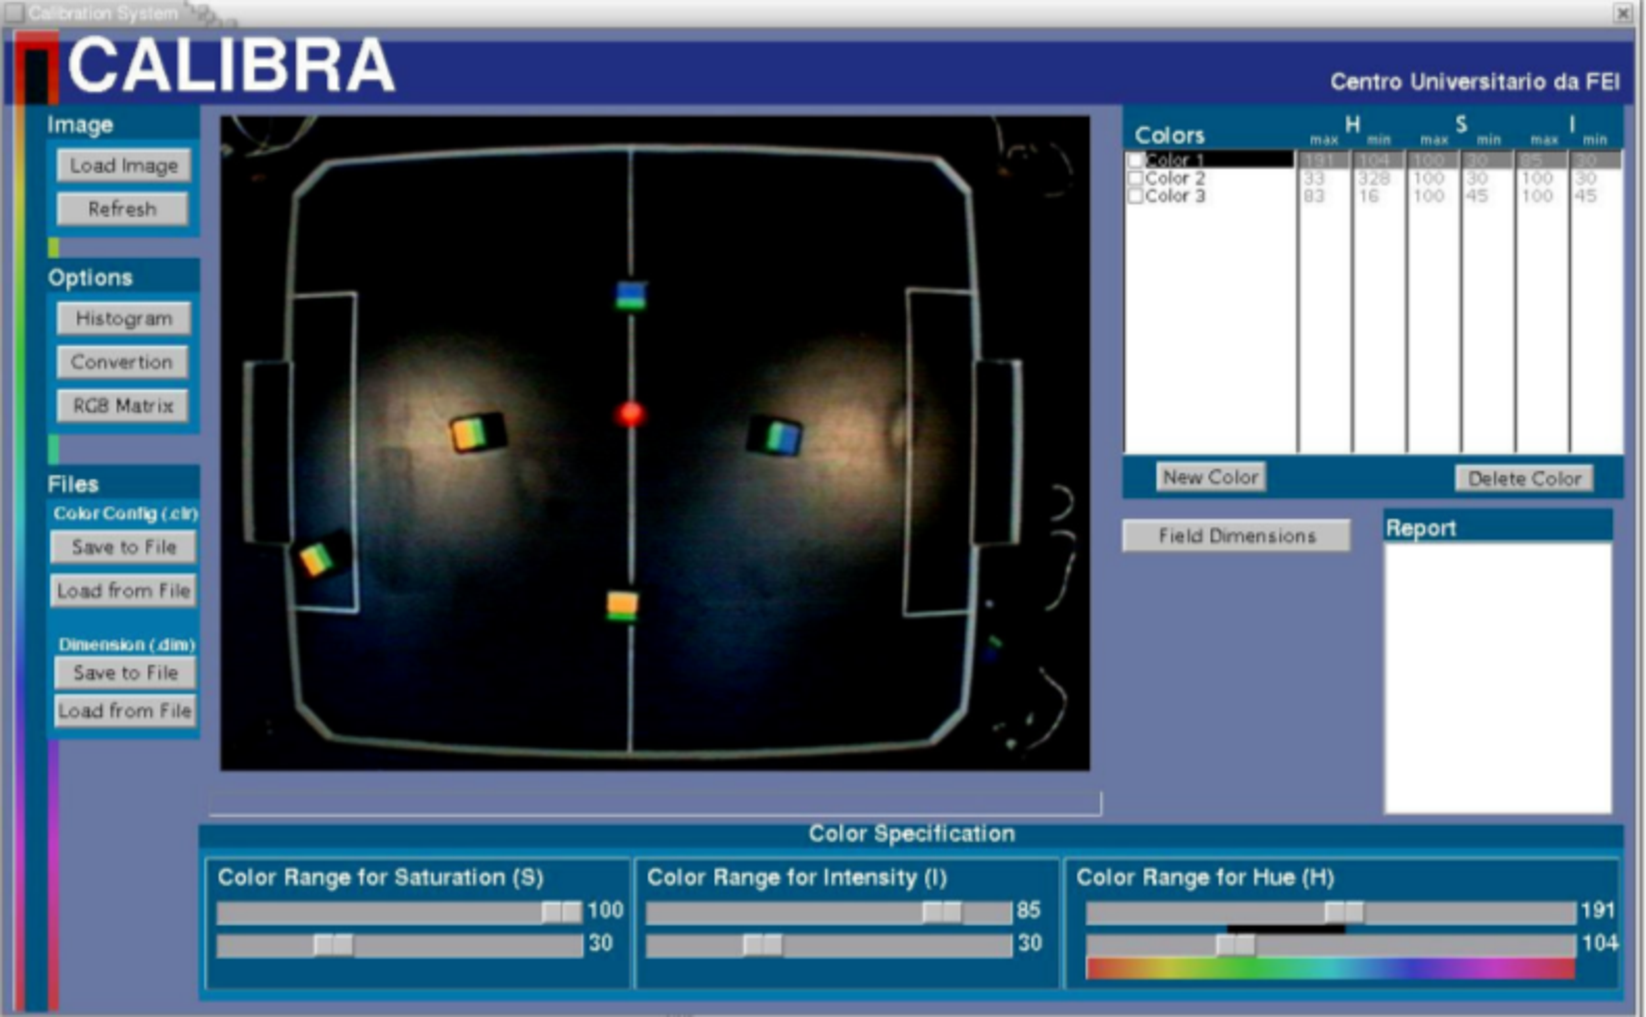
\includegraphics[width=0.6\textwidth]{calibra.pdf}
	\caption{Sistema Calibra desenvolvido pelo Centro Universitário da FEI \cite{Penharbel:2004}}
	\label{Calibra}
\end{figure}

\subsection{VSS-Vision}

Em 2015, Rosa\cite{Rosa:2015} descreveu sobre a equipe de futebol de rob\^os Very Small Size, do Laboratório de Sistemas Inteligentes e Robótica, SIRLab(Faeterj-Petrópolis), o sistema de visão computacional da equipe, durante a competição do ano de 2014, que abrange inclusive a parte de calibração. 

\begin{figure}[H]
	\centering
	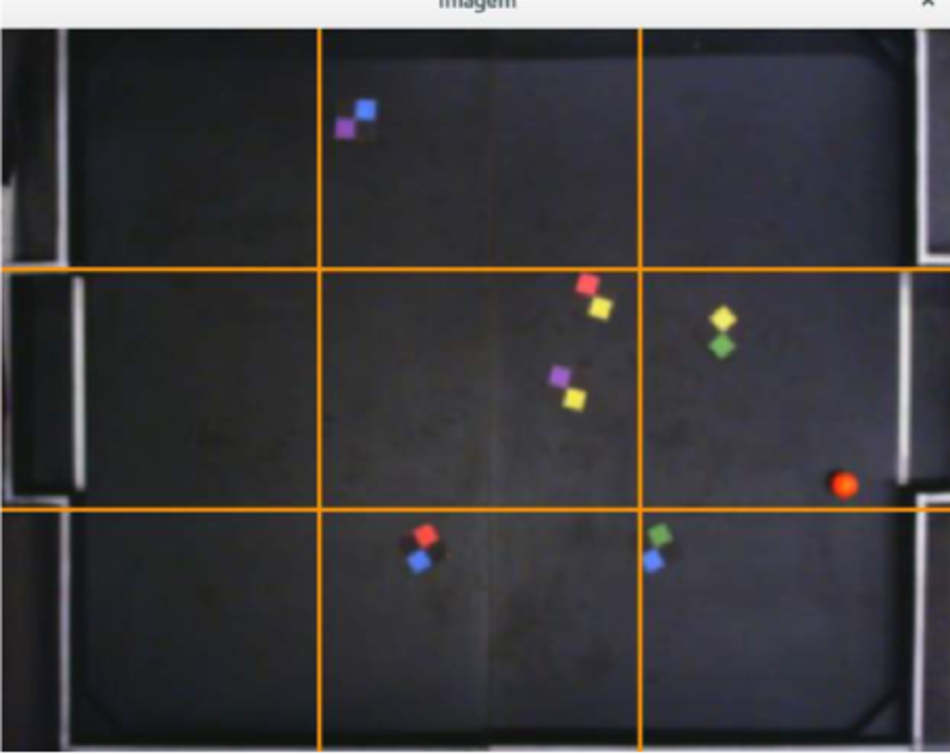
\includegraphics[width=0.4\textwidth]{vssvision.pdf} 	
	\caption{Sistema de calibracao desenvolvido peloSIRLab \cite{Rosa:2015}}
	\label{SIRLabCalibracao}
\end{figure}
Rosa menciona que a calibração de cores e feita calibrando obrigatoriamente laranja, amarelo e azul, e então as outras cores referentes aos jogadores em campo. Como visto na Figura \ref{SIRLabCalibracao} a imagem da c\^amera é dividida em nove cantos, e para calibrar a cor o usuário deve clicar em cima da cor que gostaria de ser calibrada, assim salvando um intervalo de cor tratado como RGB máximo e o mínimo daquela cor , a medida
que vão havendo os cliques o sistema verifica para cada atributo se ele é maior que o atributo
máximo salvo ou menor que mínimo salvo, caso seja, o mesmo assume o lugar de menor ou
maior\cite{Rosa:2015} e esse processo deve ser feito em cada um dos nove cantos da imagem. Os valores HSV encontrados s\~ao ajustados manualmente com a ajuda de sliders, como visto na Figura \ref{SIRLabCalibracaoHSV}. Este processo de calibração pode demorar entre cinco e dez minutos.
O desenvolvimento do sistema utiliza para processamento de imagens a biblioteca OpenCV e para telas interativas a biblioteca  ImGui.

\begin{figure}[!h]
	\centering
	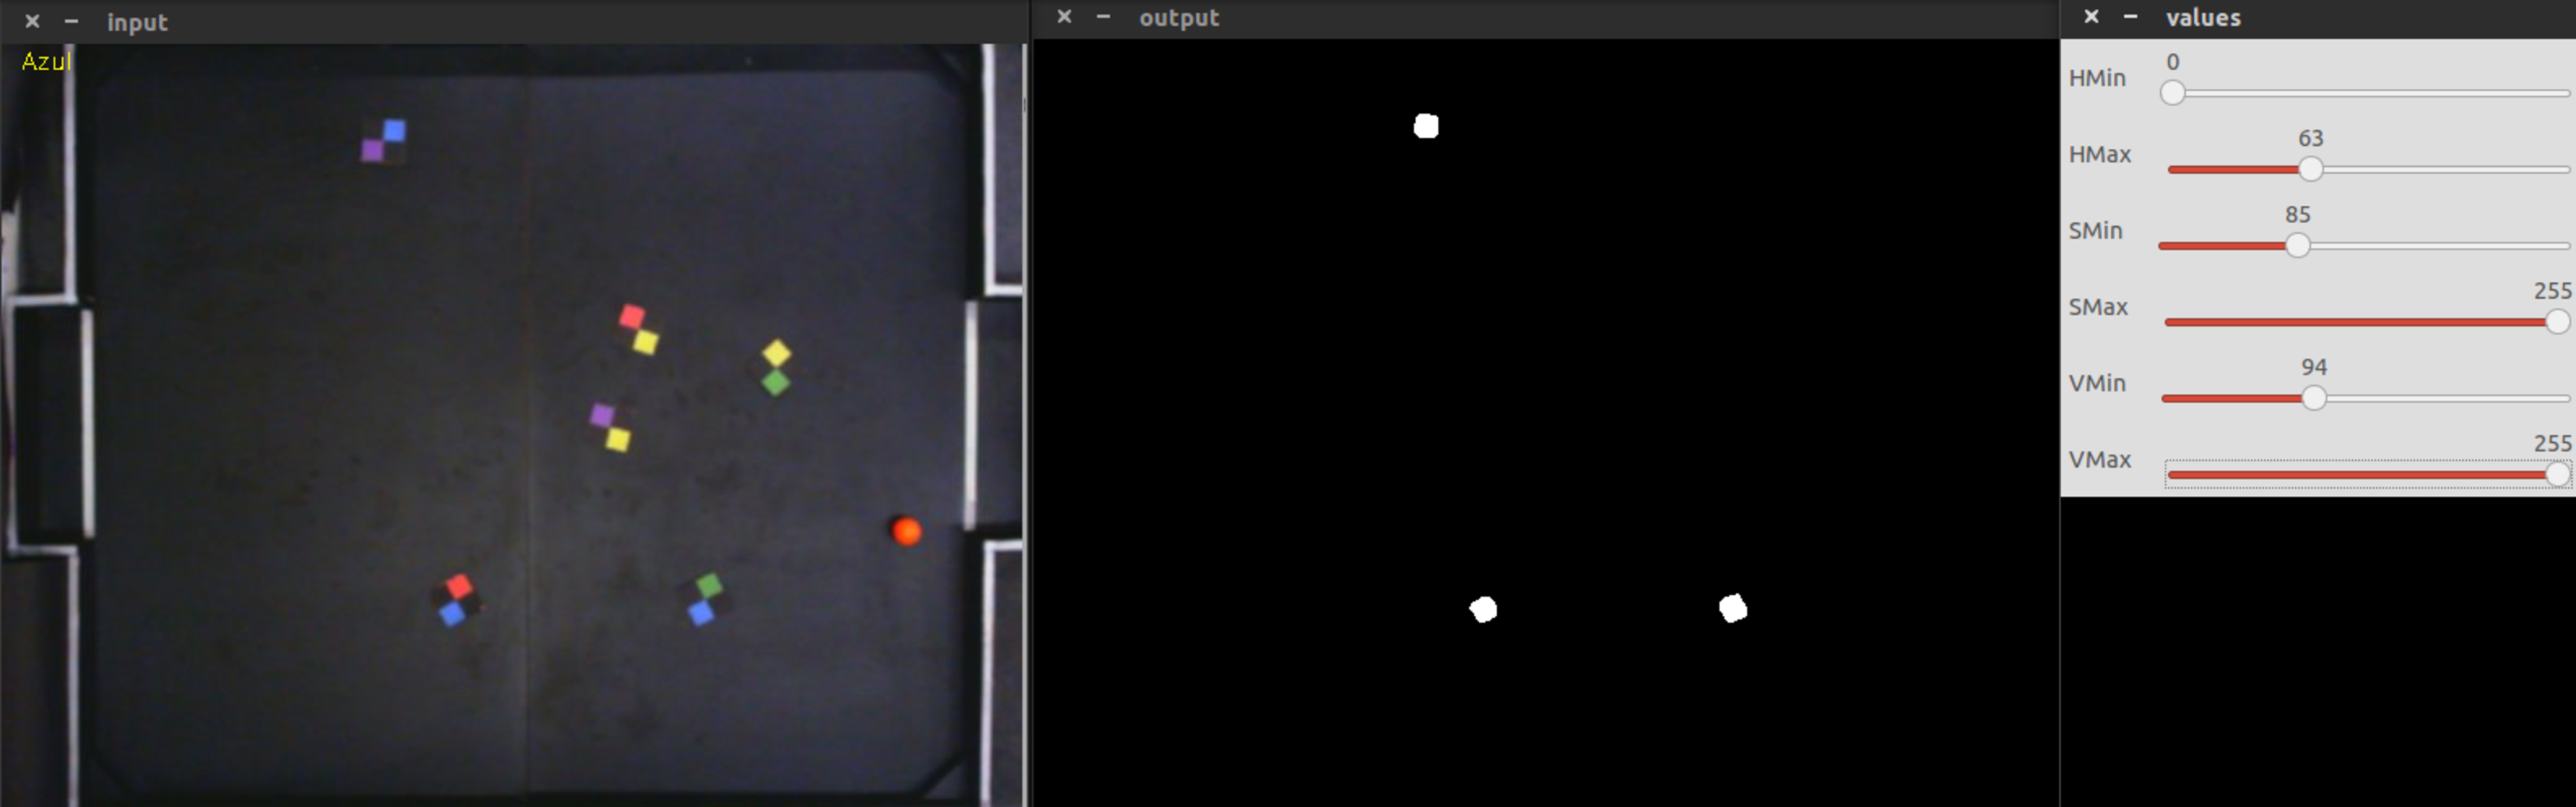
\includegraphics[width=0.8\textwidth]{calibration.pdf} 	
	\caption{Sistema de calibracao desenvolvido peloSIRLab \cite{VSSVision}}
	\label{SIRLabCalibracaoHSV}
\end{figure}

O atual sistema de visão computacional do SIRLab passou por algumas mudanças desde 2015 e conta com uma inteface e metodo de calibração diferentes\cite{VSSVision}. 
Como disponível no repositorio online do Laboratorio, o atual sistema de calibração de cores utiliza o espaço de cores HSV, no lugar do RGB\cite{Rosa:2015}. A antiga inteface do sistema, feita inicialmente em ImGui deu lugar a nova, desenvolvida em Qt, como mostra a Figura \ref{SIRLabNova}.
\


O método de calibração de cores também foi modificado, segundo a equipe\cite{VSSVision} o sistema possibilita a calibragem de 8 cores, Laranja, Amarelo, Azul, Vermelho, Verde, Rosa, Roxo, Marrom. Após o usuário escolher uma cor para calibrar o mesmo deve encontrar um intervalo de cor, no espaço de cores HSV, que represente-a. Ao clicar na tela com o botão direito o sistema da um zoom na área para ajuste fino. A Figura \ref{SIRLabNovaCalibracao} demonstra o novo método de calibração.
\begin{figure}[H]
\begin{minipage}[H]{0.45\linewidth}
\hspace{0.5cm}
\centering
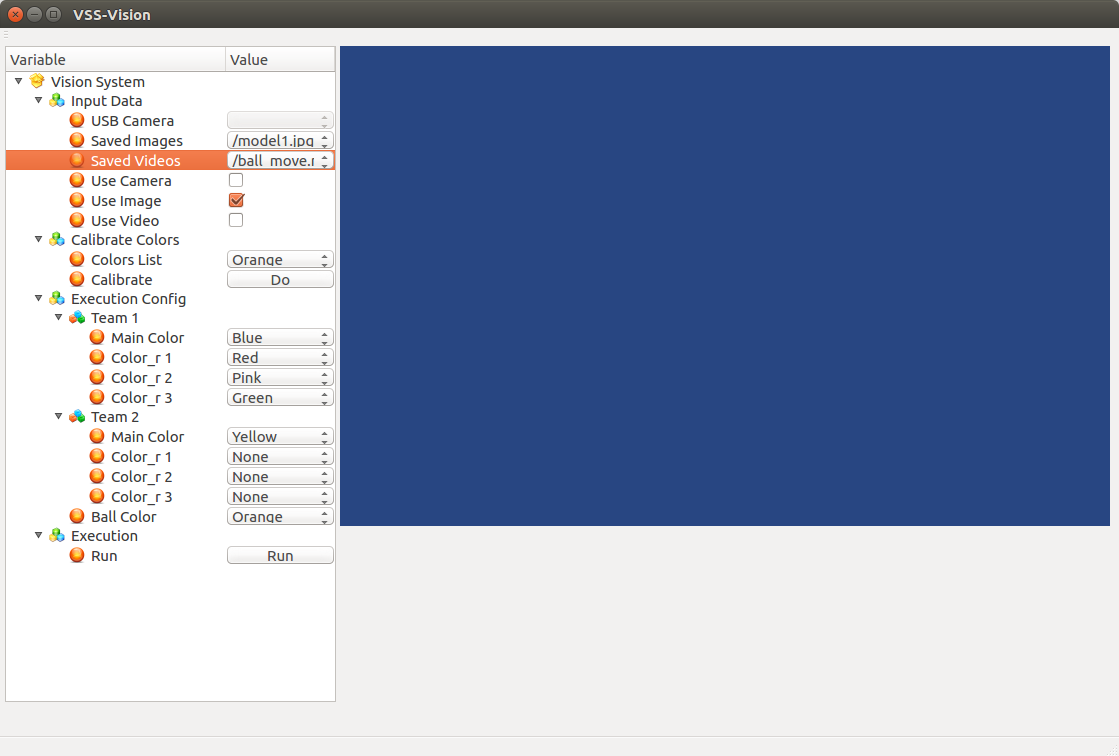
\includegraphics[width=\textwidth]{vsssnovonormal.png}
\caption{Nova interface do time da SIRLab \cite{VSSVision}}
\label{SIRLabNova}
\end{minipage}
\hspace{0.5cm}
\begin{minipage}[H]{0.40\linewidth}
\centering
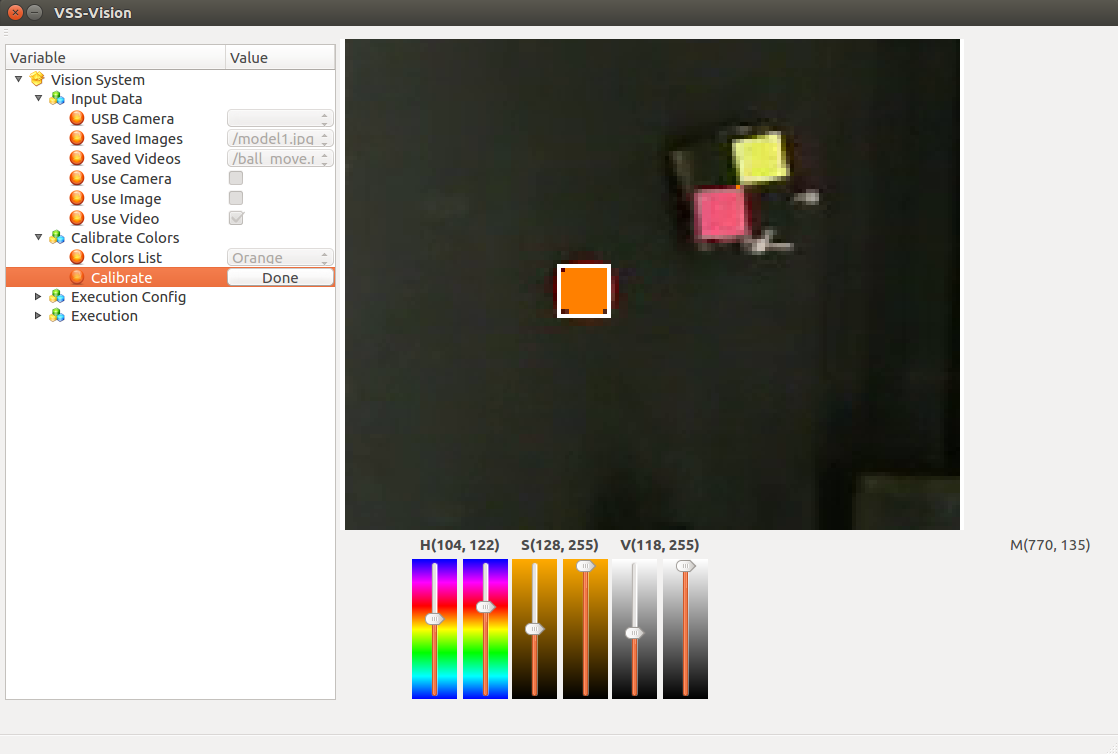
\includegraphics[width=\textwidth]{vsssnovo.png}
\caption{Calibração atual do time da SIRLab \cite{VSSVision} após calibração}
\label{SIRLabNovaCalibracao}
\end{minipage}
\end{figure}	


\section{Organização da Trabalho} \label{Sec:Organizacao}

Este trabalho está divido em cinco capítulos, incluindo esta introdução como capítulo inicial. No segundo capítulo encontra-se a fundamentação teórica do texto, contento informaç\~oes sobre processamento de imagens referente à detecção de objetos e cores. A descrição da probabilidade usada no trabalho, na descoberta do tamanho desejável dos objetos, uma breve descrição sobre o futebol de robôs. No terceiro capítulo encontra-se todo o desenvolvimento do projeto, suas classes, a descrição das tecnologias utilizadas no projeto, e o detalhamento de cada um dos tipos de calibração. No quarto capítulo são apresentados os testes e os resultados obtidos em cada um dos testes do projeto. No quinto capítulo são feitas as conclusões do trabalho e considerações finais, bem como expostas melhorias que possam vir a ser implementadas em trabalhos futuros.
 % Introdução
%====================================================================================================
% ?????
%====================================================================================================
% TCC
%----------------------------------------------------------------------------------------------------
% Autor				: Jasane Schio
% Orientador		: Gedson Faria
% Co-Orientador		: Angelo Darcy
% Instituição 		: UFMS - Universidade Federal do Mato Grosso do Sul
% Departamento		: CPCX - Sistema de Informação
%----------------------------------------------------------------------------------------------------
% Data de criação	: 01 de Outubro de 2015
%====================================================================================================
% Define o caminho das figuras
\graphicspath{{figuras/}}
\chapter{Fundamentação Teórica} \label{Cap:Fundamentacao}

%\section{Estado da Arte} \label{Sec:EstadoDaArte}
%Como estado da arte foram relacionados os métodos de detecção de objetos em imagens em tempo real e estáticas.

\section{Processamento de Imagens}
\subsection{Detecção de Objetos}
\label{Sec:TiposDeDeteccaoDeObjetos}
%Antes de descrever os métodos de classificação devemos fazer algumas definições:
%\begin{itemize}
%	\item	Em cada detecção de objetos são obtidas as informações sobre a imagem, essas são de acordo com o tipo de detecção desejada. Os dados podem conter informações como posição, tamanho, borda, transformação linear, rotação entre outros. Cada detecção em uma imagem é chamada de pose.
	
%	\item	Métodos de detecção de objeto baseado em classes constroem a classe do objeto baseada em um conjunto de treino. O conjunto de treino é composto por múltiplas imagens exemplo do objeto para que seja assim capturado os aspectos do objeto.
%\end{itemize}

A detecção de objetos pode ser considerada uma técnica herdada do reconhecimento de padrões, da área de aprendizado de máquina, esta consiste em separar objetos por categorias de acordo com uma ou mais características especificas. Quando essa técnica se junta ao processamento de imagens, onde são estas características são acentuadas em um determinado objeto dentro da imagem para assim este se destacar, tornou-se possível a detecção de objetos em imagens, que dentro do campo de visão computacional é uma das áreas que mais obtêm a atenção de pesquisadores. O primeiro Framework de métodos que usam base de dados categorizando uma ou mais características de um objetos para fazer o reconhecimento através de aprendizado foi apresentado em 2001 por Viola e Jones\cite{Viola:2001}. Desde o framework de Viola e Jones até os dias atuais muitos métodos e teorias para detecção já foram propostos e implementados como detecção de faces utilizando um classificador de redes neurais na intensidade de padrões de uma imagem, support vector machine para localizar rostos humanos e carros\cite{Nascimento:2007}, análise de componentes principais, análise independente de componentes, fatoração de matriz não-negativa, análise discriminativa linear, boosting\cite{Roth:2008}, além da classificação binaria, onde se considera a detecção do objeto em tamanho fixo apenas variando na posição na imagem\cite{AmitFelzenszwalb:2014}. 

%Em 2005 Ulusoy e Bishop\cite{Ulusoy:2005} mostraram o quão útil seria categorizar os métodos de detecção de imagens, e os dividiram em duas principais categorias: generativa e discriminativa. Categorias que foram aceitas e utilizadas como mostram Amit e Falzenszwalb\cite{AmitFelzenszwalb:2014} e Roth e Winter\cite{Roth:2008}.

%O método generativo pode ser descrito como um modelo probabilístico para a variância da pose de um objeto juntando com o modelo de aparência, ou seja, um modelo de probabilidade para a aparência da imagem condicional em uma determinada pose, juntamento com um modelo de fundo. Os parâmetros do modelo são estimados a partir de dados retirados de treinamento e as decisões são baseadas nas probabilidades anteriores\cite{AmitFelzenszwalb:2014}. Em resumo o método generativo tenta encontrar uma representação adequada dos dados originais através da aproximação dos dados originais, mas mantendo o máximo de informação possível\cite{Roth:2008}.

%Já o modelo discriminativo tipicamente constrói um classificador que pode discriminar entre imagens (ou sub-imagens) contendo o objeto e as que não contém o objeto. Os parâmetros do classificador são selecionados para minimizar os erros nos dados de treino\cite{AmitFelzenszwalb:2014}.


%	Ulusoy\cite{Ulusoy:2005} apontou as principais vantagens dos dois metodos. 
%Segundo Ulusoy e Bishop\cite{Ulusoy:2005} o método generativo se destaca por tratar perda de dados ou dados parcialmente rotulados, pela facilidade em que uma nova classe pode ser incrementada na classificação condicional de densidade, independentemente das classes anteriores, e por conseguir facilmente lidar com composição de objetos (ex: óculos, chapéus...), considerando que os modelos discriminativos precisar analisar todas as combinações durante o treinamento. Amit e Felzenszwalb\cite{AmitFelzenszwalb:2014} ainda aponta que as vantagens descritas sobre o método discriminativo são ditas como a flexibilidade do modelo  que pode ser utilizado em regiões do espaço de entrada onde as probabilidades posteriores diferem significativamente de 0 ou 1, ao passo que as abordagens detalhes generativas modelo de distribuição de X, que podem ser irrelevantes para determinar as probabilidades posteriores, além de ser tipicamente muito rápido em fazer previsões para os novos pontos (teste) de dados, enquanto os modelos generativos muitas vezes exigem solução iterativa, e pela igualdade de circunstâncias, seria de esperar que os métodos discriminativos tenham melhor desempenho preditivo, uma vez que são treinados para prever o rótulo de classe em vez de a distribuição conjunta de vetores e alvos de entrada.

\subsection{Detecção de Bordas}
Para um objeto poder ser detectado por algum método de detecção a imagem passa por um processo de segmentação. A segmentação pode ser dita como o processo de divisão da imagem em objetos\cite{Gonzalez:2008}. De acordo com Wangenheim\cite{Wangenheim:2014} o processo de segmentação se baseia em dois conceitos: similaridade e descontinuidade. A descontinuidade é o processo onde se separa o fundo das partículas e estas umas das outras, através de linhas, bordas ou pontos. Já a similaridade é o processo onde os pixeis provenientes da descontinuidade são agrupados de acordo com a proximidade um dos outros para formar os objetos de interesse. De acordo com Canny\cite{Canny:1986} o processo de detecção de bordas é um processo simplificado que serve para diminuir drasticamente o total de dados a serem processados e ao mesmo que o mesmo preserva informações valiosas sobre os objetos, este tambem é considerado um processamento de imagem de baixo nivel, uma vez que age diretamente na imagem original apenas melhorando-a. É muito comum a ocorrência de ruídos quando se trata da detecção de bordas, e por sua vez para evitar esses ruídos é necessário a suavização da imagem antes de fazer a detecção. Vale\cite{Vale:2002} lembra que a suavização possui pontos negativos como perda de informação e deslocamento de estruturas de feições proeminentes no plano da imagem. Além disso, existem diferenças entre as propriedades dos operadores diferenciais comumente utilizados, o que ocasiona  bordas diferentes.Assim, como dito por Ziou e Tabbone citados por Vale\cite{Vale:2002}, se torna difícil encontrar um algoritmo que tenha bom desempenho em diferenciados contextos e capture os requisitos necessários aos estágios subsequentes do processamento. 
Quando se trata de detecção de bordas existem dois critérios\cite{Canny:1986} para essa detecção que devem ser levados em consideração, Taxa de Erro e Localização\cite{Vale:2002}. 
\begin{description}
	\item[Taxa de Erro] É importante que as bordam contidas na imagem não sejam confundidas ou perdidas e ainda que não sejam detectadas bordas falsas. É necessário que o algoritmo de detecção de borda tenha uma baixa taxa de erro para que seja eficiente.\cite{Wangenheim:2014, Canny:1986, Vale:2002}
	\item[Localização] A distância entre os pixels de borda encontradas pelo algoritmo e a borda atual deveriam ser o menor possível.\cite{Wangenheim:2014}
\end{description}
Ao tentar aplicas esses dois critérios para desenvolver um modelo matemático para detecção de bordas sem a necessidade de base em regras preestabelecidas em seu artigo
\textit{ A Computational Approach to Edge Detection} Canny percebeu que somente esses dois critérios não eram o suficiente para obter uma boa precisão da detecção de bordas. E então propôs um terceiro critério: Resposta.
\begin{description}
	\item[Resposta] Para contornar a possibilidade de mais de uma resposta para a mesma borda, ou seja o detector de bordas não deveria identificar múltiplos pixels de borda onde somente exista um único pixel. \cite{Wangenheim:2014, Canny:1986, Vale:2002}
\end{description}


Com o acréscimo do terceiro critério então nota-se que o processo de detecção de bordas de Canny
mostrou-se bastante flexível, independente da origem da imagem utilizada\cite{Vale:2002}.
 \begin{figure}[!h]
	\centering
	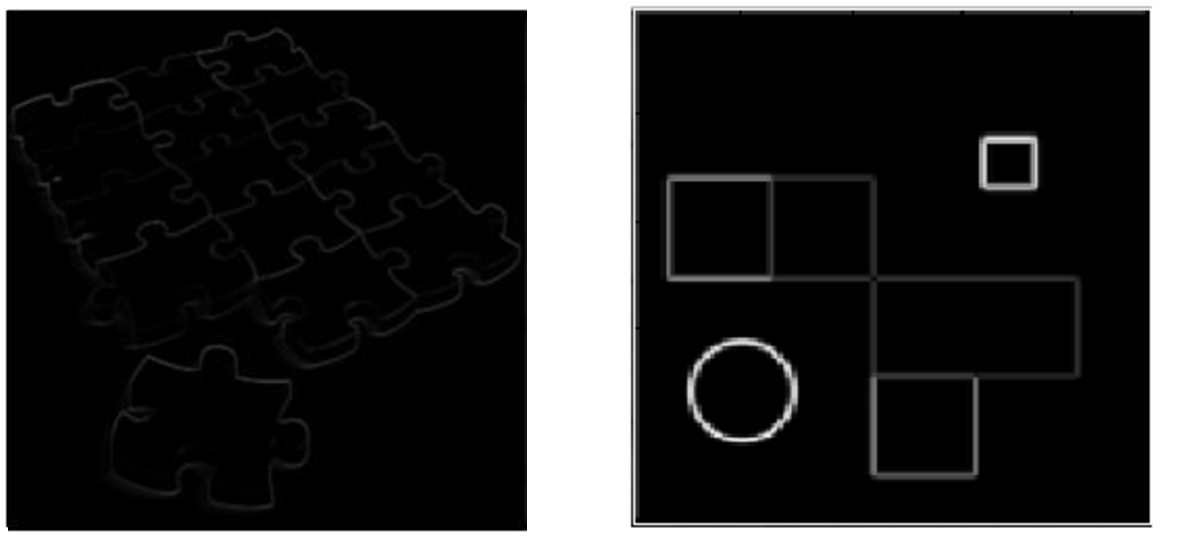
\includegraphics[width=0.8\textwidth]{canny.pdf}
	\caption{Detecçcao de Borda com Algoritmo de Canny \cite{Saini:2013} }
	\label{Canny}
\end{figure}







\section{Cores} \label{Sec:Cores}


O olho humano é capaz de identificar cores mesmo com as mais diferentes interferências, luminosidade, tonalidade, intensidade, entre outras ações de agentes externos graças aos \textbf{cones} e \textbf{bastonetes}. Os bastonetes são os responsaveis por distinguirem tons de cinza e pela visão periferica e tem como caracteristica serem sensiveis a baixo nivel de luminosidade\cite{Azevedo:2003}, os cones, por sua vez, são sensiveis ao alto nivel de iluminação e responsaveis pela percepçao de cores\cite{Azevedo:2003}. Segundo a teoria tricomática de Thomas Young e mais tarde estudada por Hermann von Helmholtz\cite{Azevedo:2003}, a retina humana é formada por três tipos de fotopigmentos que seriam os três receptores de cor, ou seja respondiam ao comprimento de onda de apensa três cores: Vermelho, Verde e Azul. A informação obtida através do sistema visual humano é assimilada pelo nosso cérebro e ligando a cor a sua aparência levando em consideração o aprendizado que obtivemos sobre a mesma, já para uma máquina cores são números, códigos, cada cor contém um código especifico e cada uma de suas variâncias também. Para o nosso cérebro é muito fácil entender, exemplo, que o verde, verde lima, verde escuro são todos verde, apenas com tonalidades diferentes, já para o computador estas são: (0,255,0),(50,205,50),(0,128,0), no padrão de cor RGB. Mas se for aplicado luminosidade nessas cores, por exemplo, elas ainda se tornam outras diferentes cores, um código diferente para cada luminosidade possível.




Para poder explicar as propriedades e comportamentos das cores em determinadas circunstâncias, surgiram os \textbf{Sistemas de cores}. Devido a complexidade existente em explicar todos os aspectos relacionados às cores são utilizados diversos sistemas para descrever as mais diferentes caracteristicas das cores e sua percepção pelo ser humano\cite{Azevedo:2003}.  Dentro os sistemas mais conhecidos, estão o RGB, HSV E HSL, sistemas quais falaremos neste trabalho.

Segundo Azevedo\cite{Azevedo:2003} o universo de cores que podem ser reproduzidas por um sistem é chamado de \textbf{Espaço de Cores}. De acordo com Foley et. al citado por Souto\cite{Souto:2003} espaço de cores é um sistema tridimensional de coordenadas, onde cada eixo refere-se a uma cor primária. A quantidade de cor primária
necessária para reproduzir uma determinada cor, é atribuída a um valor sobre o eixo
correspondente. O espaço de cores pode ser entendido como a quantidade de detalhamento, tonalidades de uma cor, dentro do espectro de cores de um determinado modelo de cor.

 \begin{figure}[!h]
	\centering
	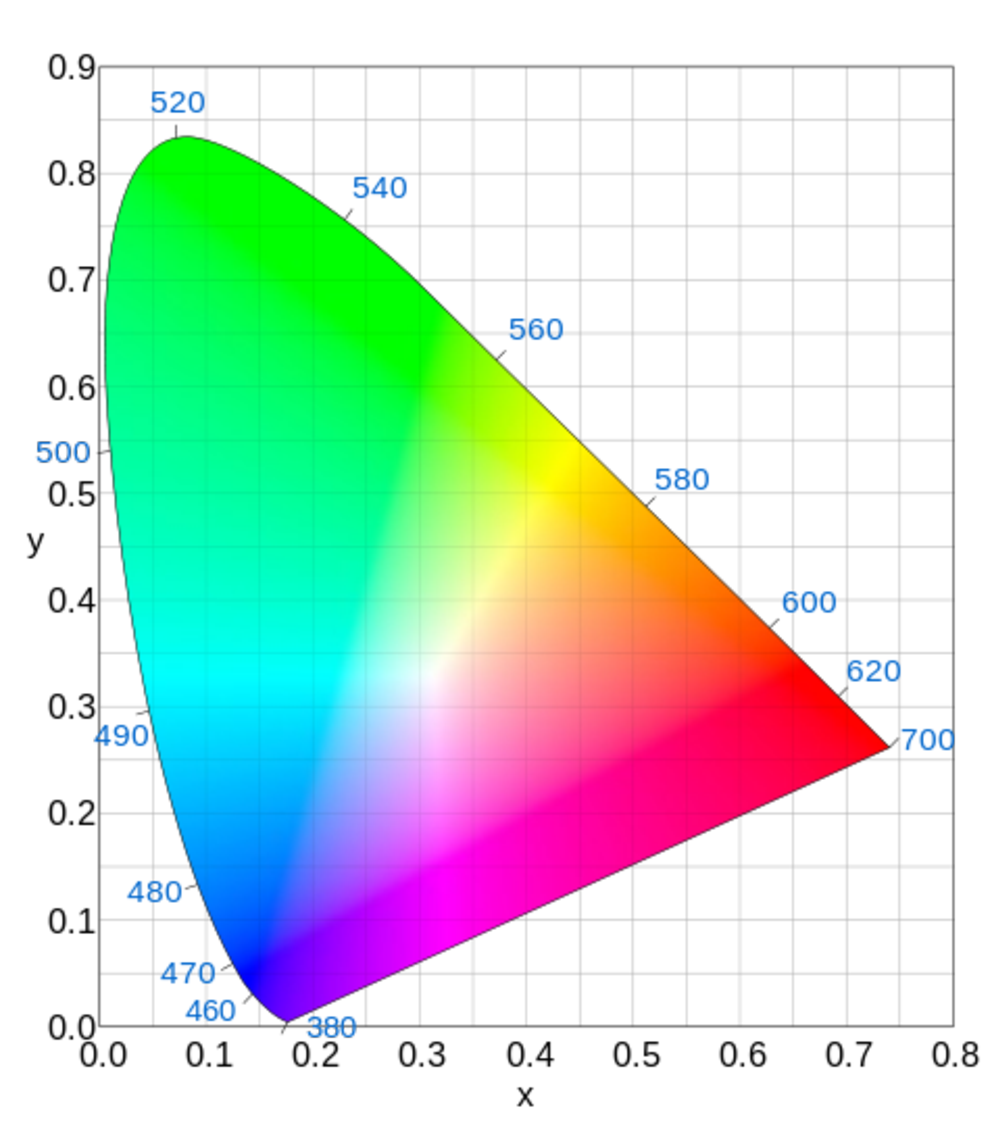
\includegraphics[width=0.25\textwidth]{graficocie.pdf}
	\caption{Universo de cores estabelecido pelo CIE.}
	\label{EspacodeCores}
\end{figure}


Quando fez sua primeira experiência com a decomposição da luz em um prisma para obter cores Newton percebeu que não havia a cor branca. Ele tentou então misturar as sete cores que obteve para gerar a branca, sem sucesso. 
 Para conseguir cobrir todas as alterações e caracteristicas as cores em 1921 a Comissão Internacional de Iluminação (CEI)\cite{Souto:2003} definiu três primarias(X, Y e Z) que podem ser combinadas para formarem todas as cores e entendeu-se que existe duas formas de se obter cores: através da emissão ou reflexão de luz, espaços RGB e CMY respectivamente, \figurename{ 2.2}. Assim entendeu-se então porque em seu experimento Newton não obteve sucesso para gerar a cor branca, pois parar gerar a cor branca é necessário a soma das três cores primarias azul, verde e vermelho, uma vez que seu experimento utilizava a reflexão e não emissão de cores.
 \begin{figure}[!h]
	\centering
	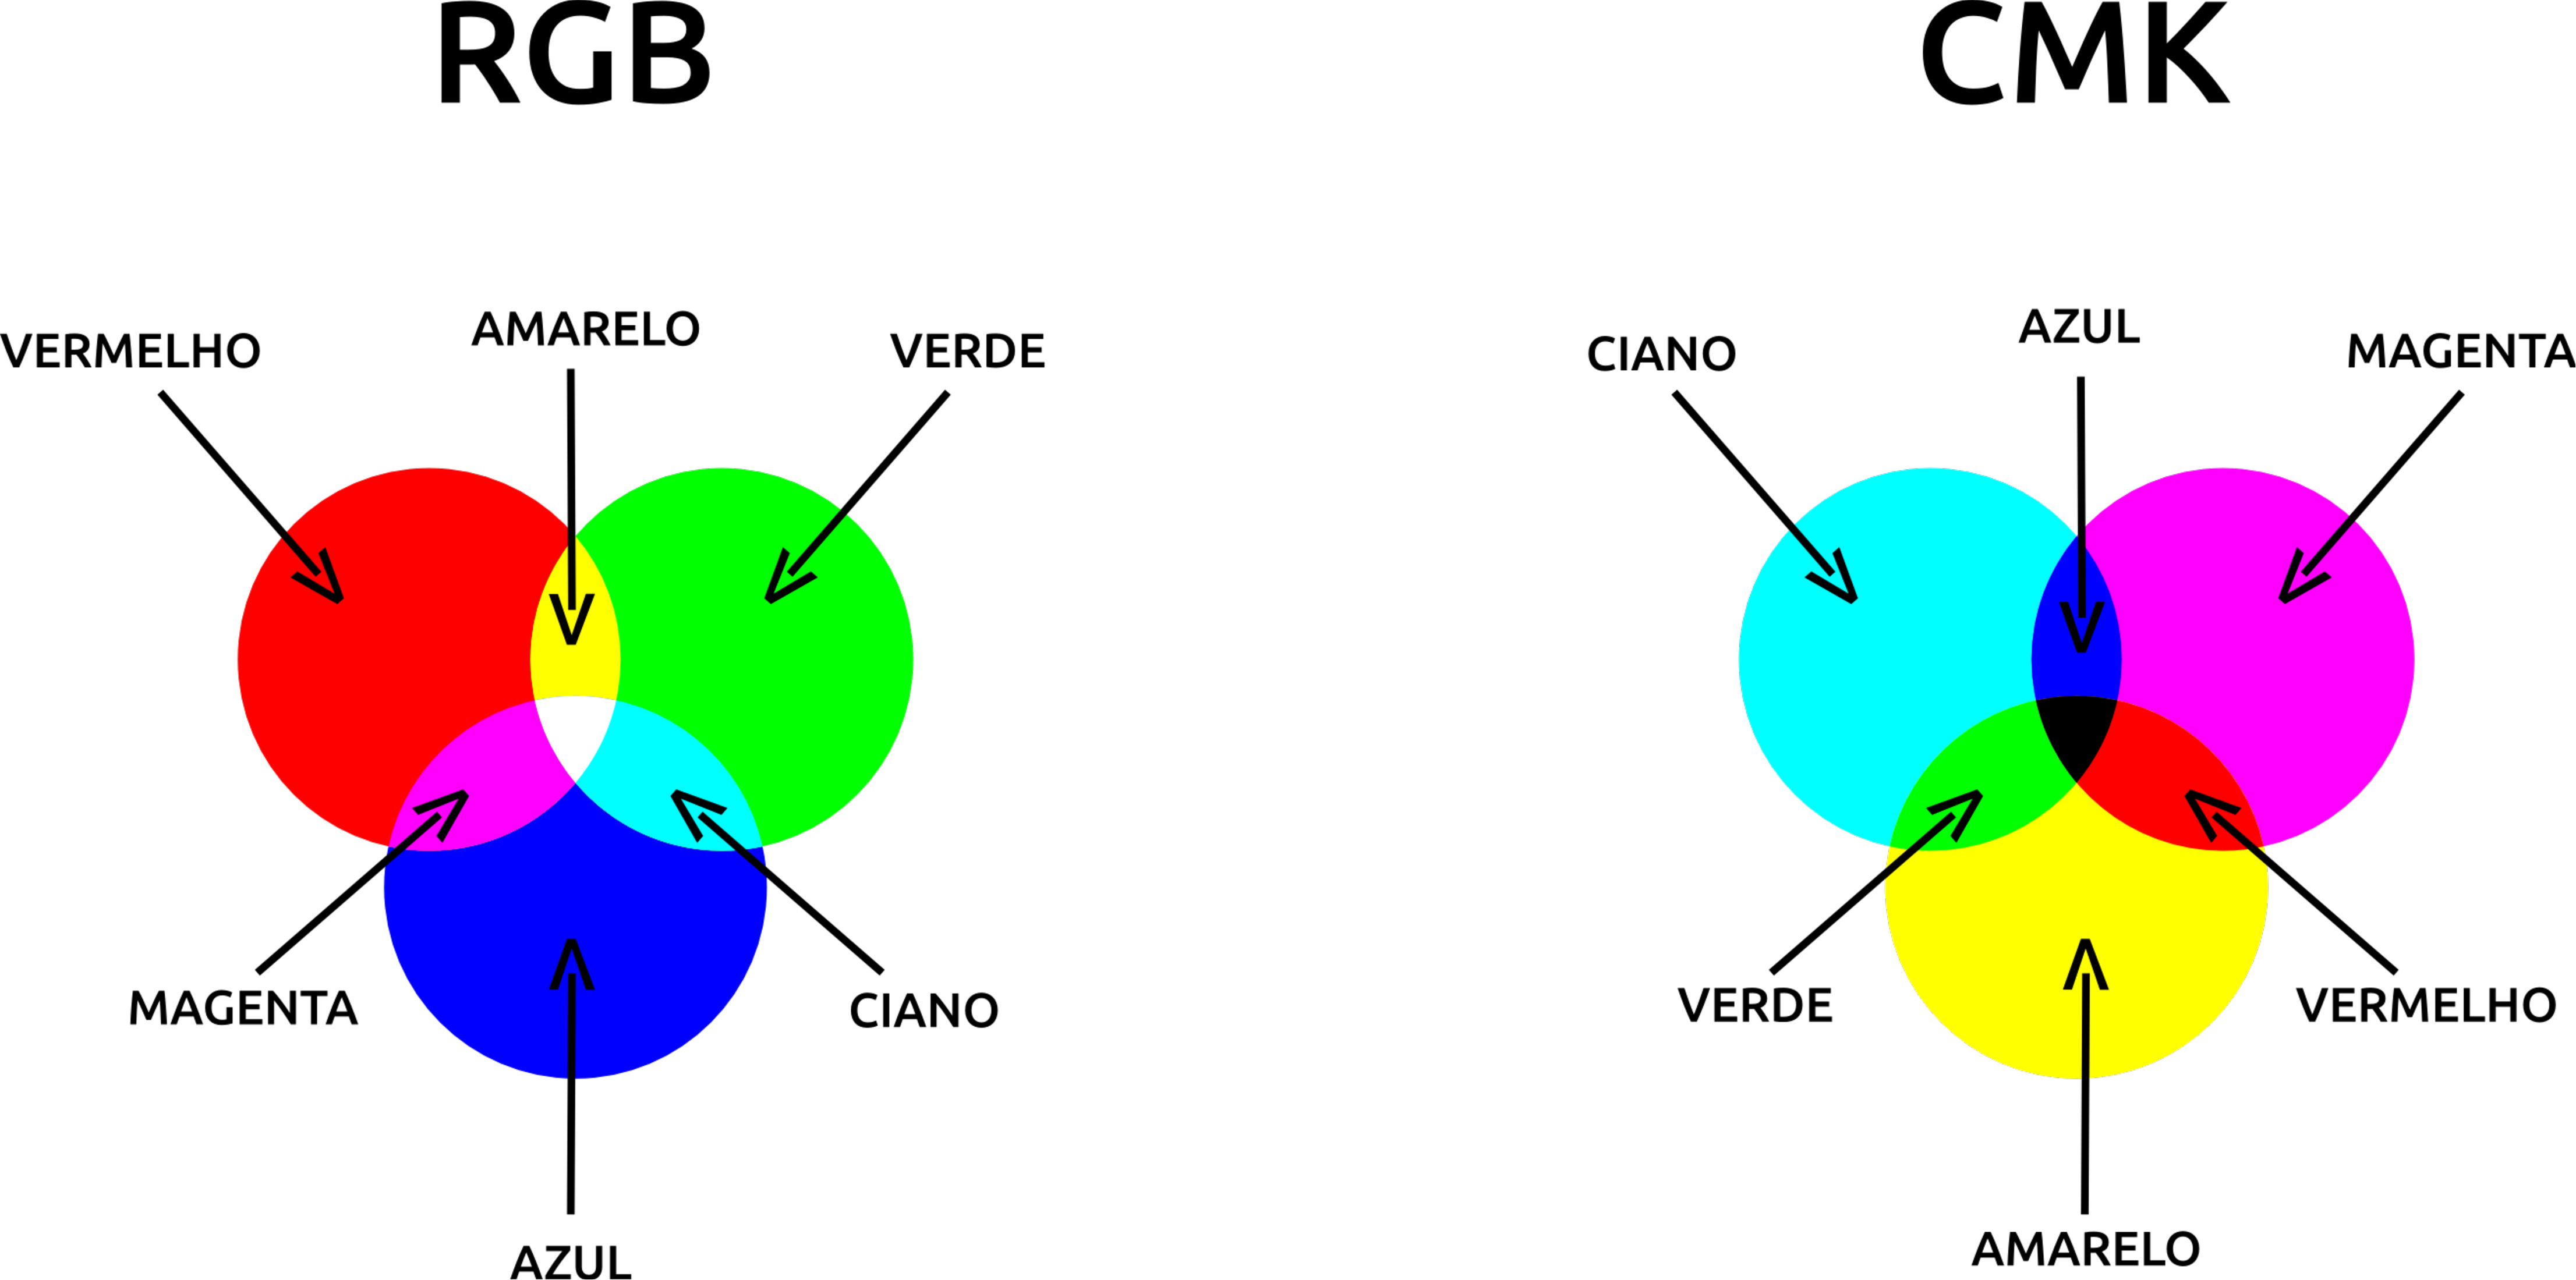
\includegraphics[width=0.5\textwidth]{espacos.pdf}
	\caption{Exemplo dos espaços de cores RGB E CMY.}
	\label{EspacodeCores}
\end{figure}



Para utilização pratica de sistemas e espaços de cores e descreverem as cores foram criados modelos de cores, neste trabalho falaremos sobre o RGB e HSV, pois são os modelos usados durante o desenvolvimento.
Modelo de cores são modelos matemáticos utilizados para classificação das cores de acordo com sua tonalidade, saturação, luminosidade ou crominância na tentativa de conseguir cobrir o maior número de cores possíveis e assim simulando a visão. A representação da cor é definida por um único ponto em um modelo tridimensional. 
Os modelo de cores tem função definir as cores nos programas gráficos de computadores de forma que combine com a 
percepção das cores pelo sistema visual humano e utiliza três eixos similares para definirem a cor\cite{Leao:2005}.

O modelo de cores RGB pode ser considerado mais básico dos modelos de cores. Seu nome possui a mesma definição do espaço de cores RGB. Ele não utiliza de nenhum atributo como luminosidade ou tonalidade, por exemplo, para a definição da cor apenas a adição das cores primarias, azul, verde e vermelho. É este também o padrão mais usado e conhecido. Os valores de R,G e B variam de 0 à 255.


\begin{figure}[!h]
	\centering
	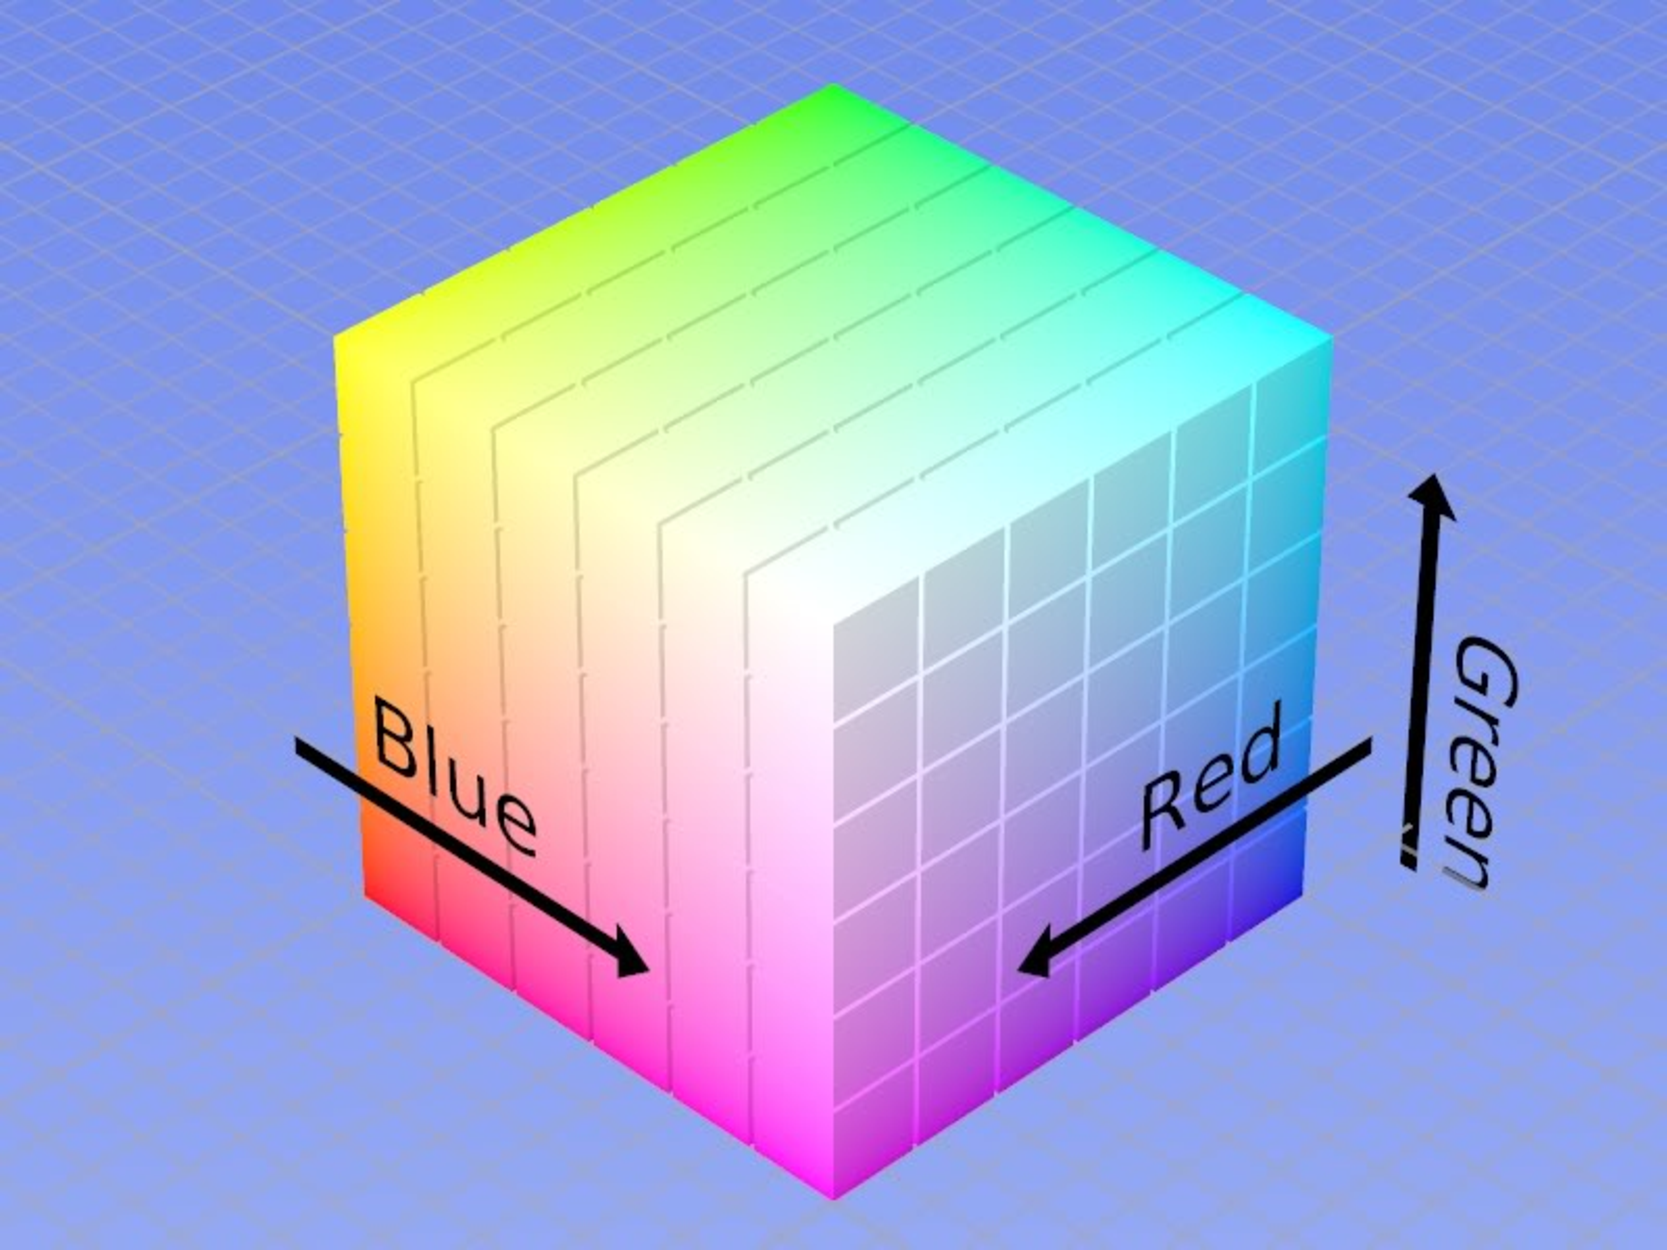
\includegraphics[width=0.4\textwidth]{rgb.pdf}
	
\caption{Exemplo do Modelo de Cor RGB.	 Horvath\cite{ImagensHSLHSVRGB}  }
	\label{ModeloRGB}
\end{figure}



O modelo HSV define tonalidade (hue) que é a cor em si, variando de 0 a 360º, a saturação(saturnation) que define o grau de pureza da cor, variando de 0 a 1, obtido pela mistura da tonalidade com a cor branca e brilho (value) que tenta fazer referência à percepção humana\cite{Leao:2005} que é a intensidade da cor, escala de tons de cinza\cite{Azevedo:2003}, variando também de 0 a 1.


\begin{figure}[!h]
	\centering
	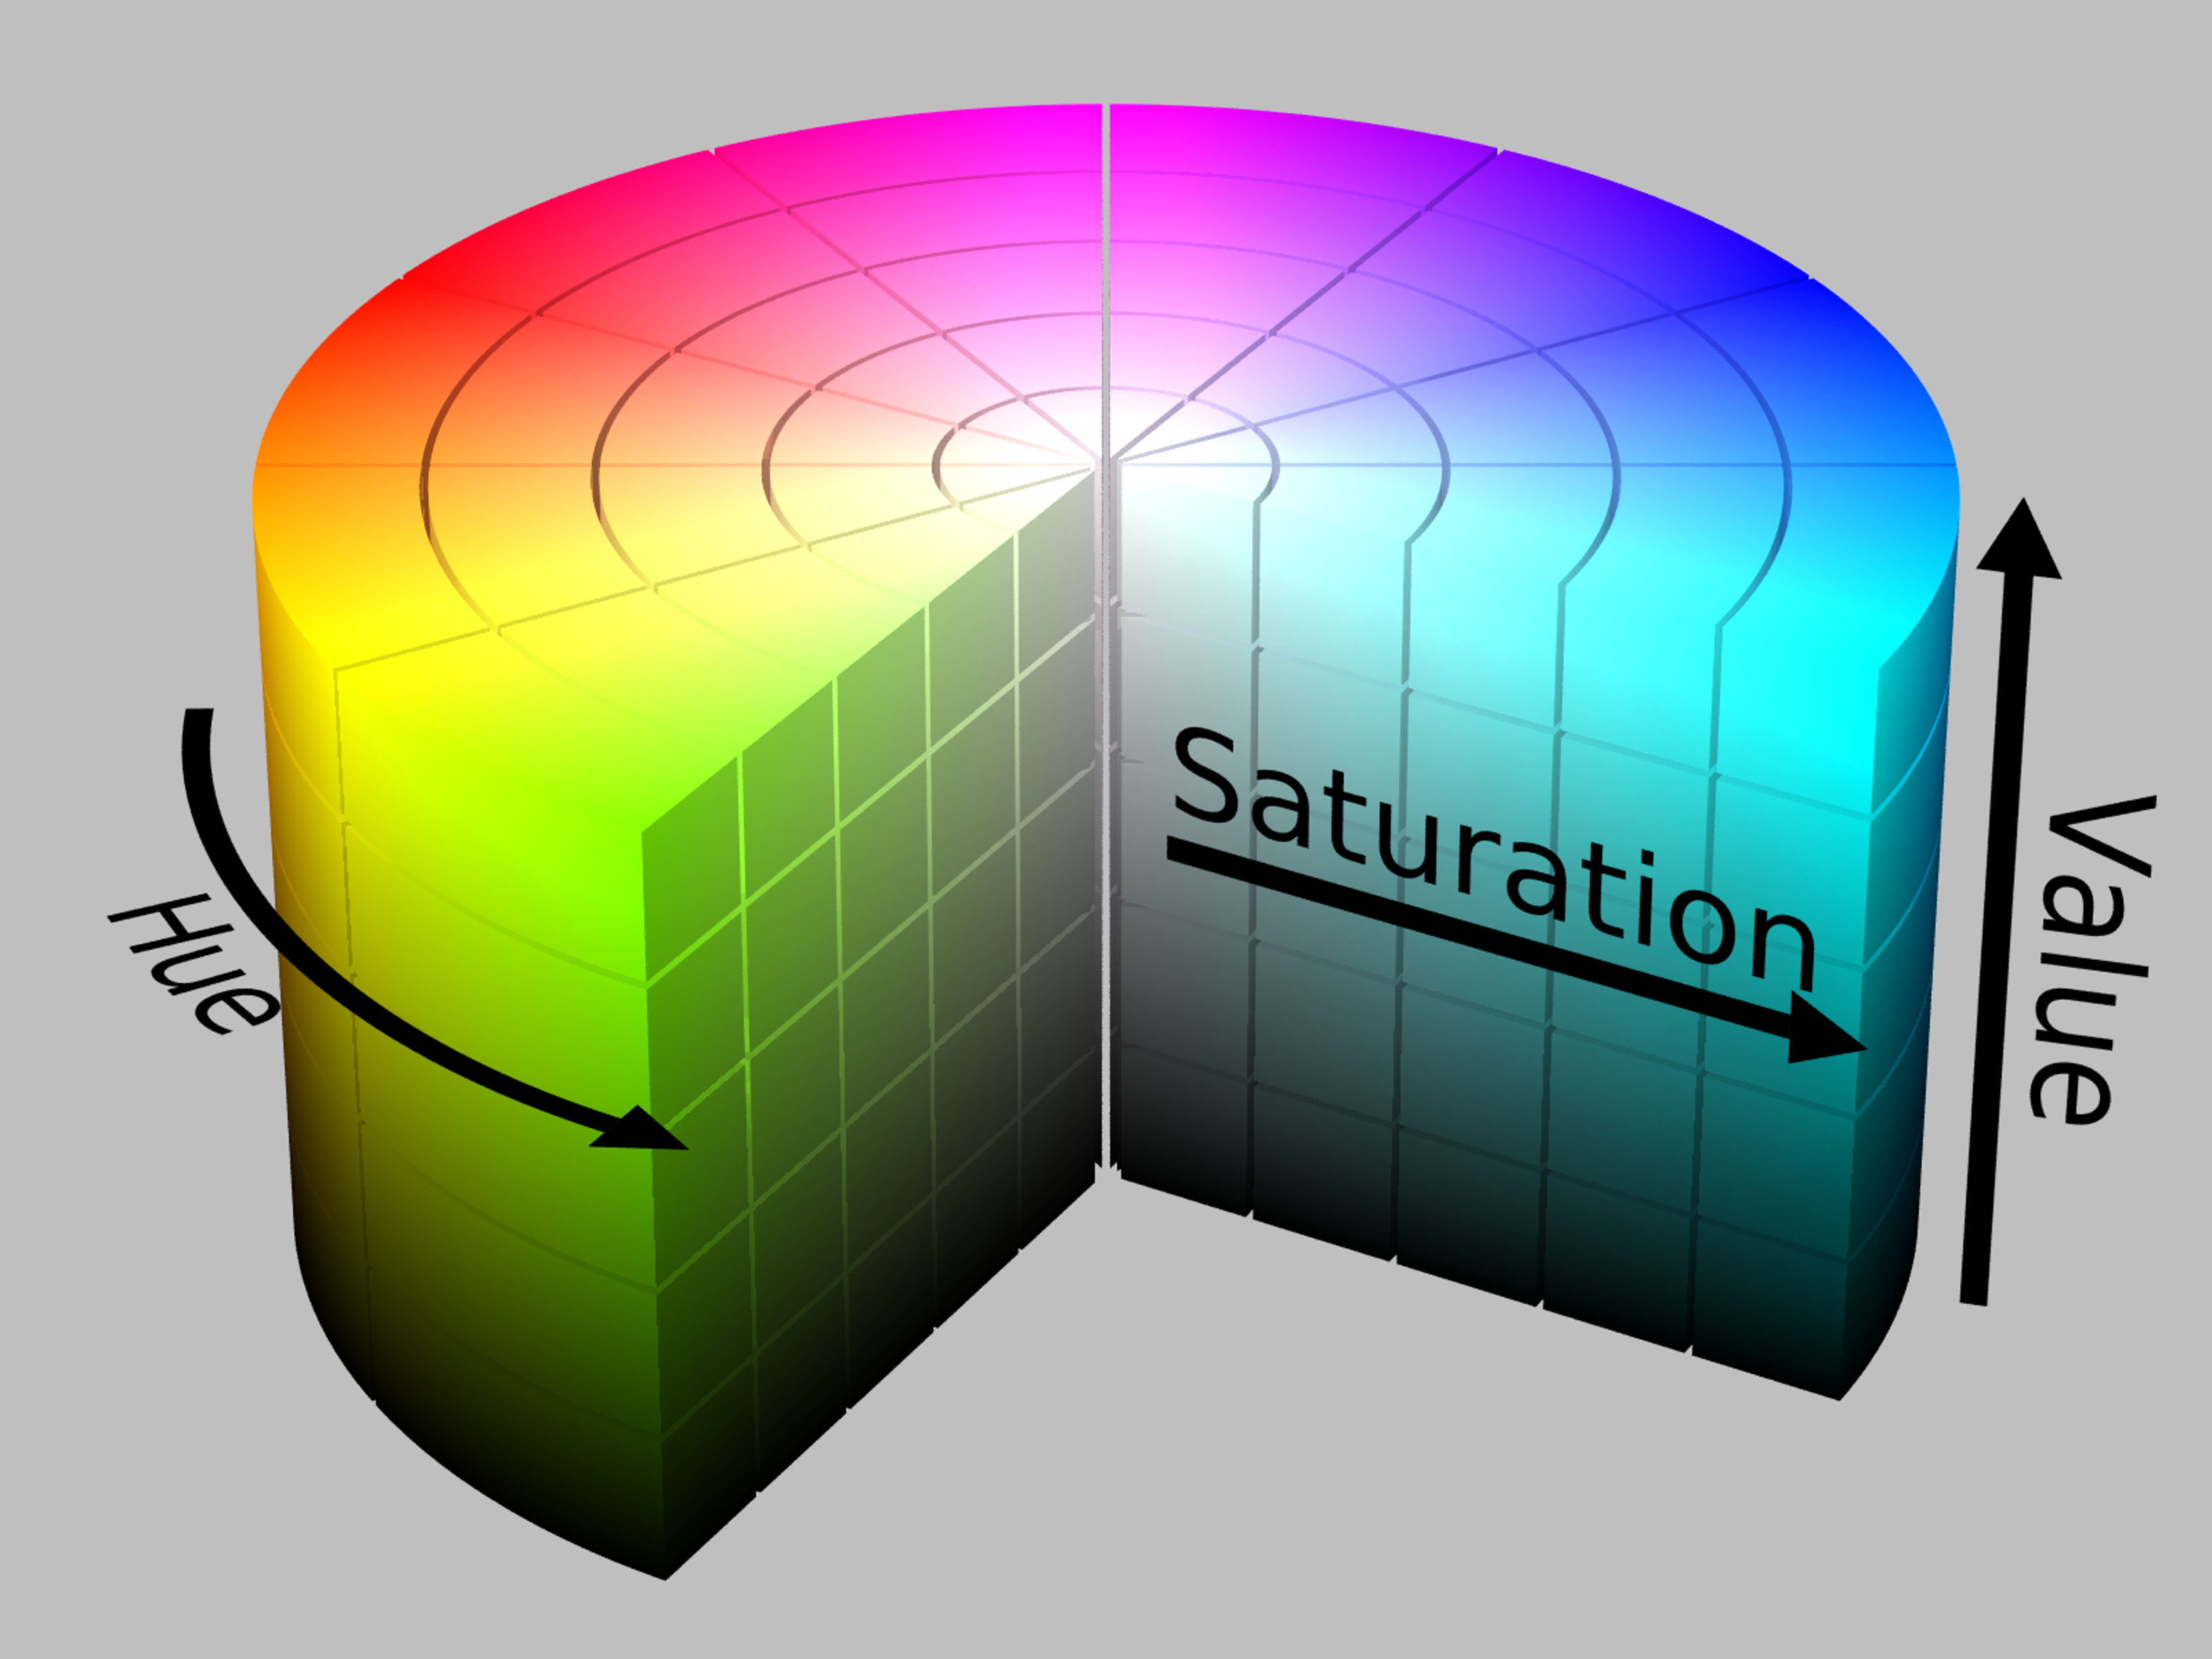
\includegraphics[width=0.4\textwidth]{hsv.pdf}
	
	\caption{Exemplo do Modelo de Cor HSV, Horvath\cite{ImagensHSLHSVRGB}}
	\label{ModeloHSV}
\end{figure} 


O sistema HSV utiliza definições de cor mais intuitivas que o conjunto de cores primarias, por isso são mais adequados quando se necessita obter varias tonalidades.

\section{Futebol de Robôs}
 Visto como um dominio bastente complexo, dinamico e imprevisivel\cite{Costa:2000}, o futebol de robos surgiu como uma tentativa de promover pesquisas nos campos de Inteligencia Artificial e robotica, pela avaliacao teorias, algoritmos e arquiteturas atraves problemas padrao\cite{Kitano:1997}.
 A Equipe Cedro se enquadra na categoria IEEE Very Small Size. Esta categoria é regulamentada pelo Instituto de Engenheiros Eletricistas e Eletrônicos (IEEE) e possui regras baseadas na MiroSot\cite{Rosa:2015}. O futebol de robôs se assemelha ao futebol humano onde o objetivo do jogo é fazer gols para vencer a partida, porem tendo regras adaptadas para o "âmbito" robótico. 
 Rosa\cite{Rosa:2015} em seu trabalho de graduação faz uma boa enumeração das regras básicas:
 \begin{itemize}
 \item A partida dura 10 minutos com dois tempos de 5 minutos;
  \item Há um intervalo de 10 minutos entre um tempo e outro;
   \item Cada time tem direito a dois tempos de 2 minutos que podem ser pedidos a qualquer
   momento;
    \item Caso a diferença de gols entre os dois times chegue a 10 a partida é encerrada;
     \item Uma falta ocorre quando há mais de um robô de um mesmo time dentro de sua própria
     área de gol ou quando um robô empurrar outro robô de outro time;
     \item Um pênalti ocorre quando a bola fica mais de 10 segundos dentro de alguma das áreas;
     \item Um chute-livre ocorre quando os robôs ficam travados por mais de 10 segundos, caso
     ocorra, o juiz posiciona a bola na marca de chute-livre mais próxima de onde ela ficou
     parada e posiciona os robôs de cada time equidistantes a bola;
     \item A cada inicio de partida ou gol feito a bola deve ser posicionada no centro do campo e os
     robôs devem ser posicionados de acordo com a posse de bola.
 \end{itemize}

%\section{Trabalhos Relacionados}
%Para o tema especifico deste trabalho, calibração de intervalo de cores para times de futebol de robos da categoria very small size, não foram encontrados trabalhos relacionados, porém foram encotrados Team Discription Papers e descrições de sistemas usados pelos times, onde consta sobre o processo de calibração e os metodos usados.
%
%\subsection{Calibra}
%O Centro Universitário da FEI, como visto em\cite{PenharbelTime}, utiliza em sua equipe Y04 utiliza um sistema, desenvolvido denominado CALIBRA\cite{Penharbel:2004}.Desenvolvido para sistemas Linux e com Graphical User Interface\cite{Penharbel:2004}, o sistema de calibração possui um modulo chamado de MainWindow, que é responsavel pela configuracao de brilho, cor e contraste da imagem adquirida pela camera e gera um arquivo que é analizado na hora da criacao das cores padrao\cite{PenharbelTime}, onde cores-padrão são definidas como intervalos no espaço de cores HSI\cite{PenharbelTime}.
%
%\begin{figure}[!h]
%	\centering
%	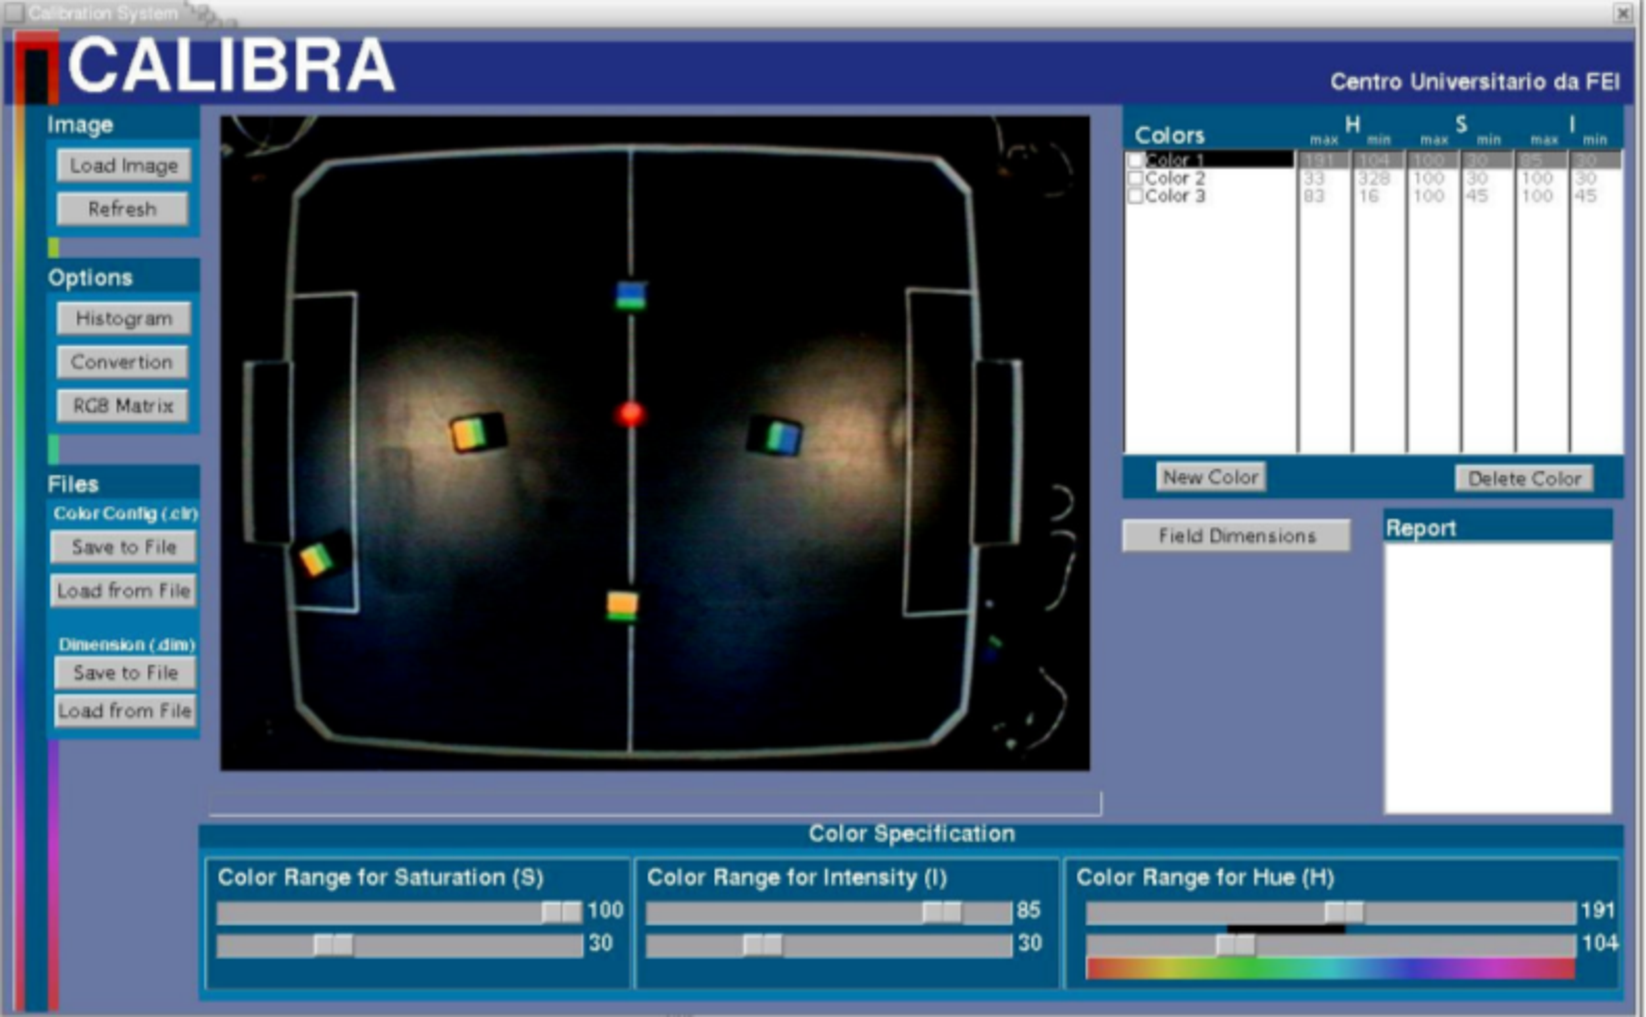
\includegraphics[width=0.6\textwidth]{calibra.pdf}
%	\caption{Sistema Calibra desenvolvido pelo Centro Universitário da FEI \cite{Penharbel:2004}}
%	\label{Calibra}
%\end{figure}
%
%\subsection{VSS-Vision}
%
%Em 2015 Rosa\cite{Rosa:2015} descreve em seu Trabalho de Conclusão sobre a equipe de futebol de rob\^os Very Small Size, do Laboratório de Sistemas Inteligentes e Robótica, SIRLab(Faeterj-Rio), o sistema de visão computacional da equipe, durante a competição do ano de 2014, que abrange inclusive a parte de calibração. 
%
%\begin{figure}[!h]
%	\centering
%	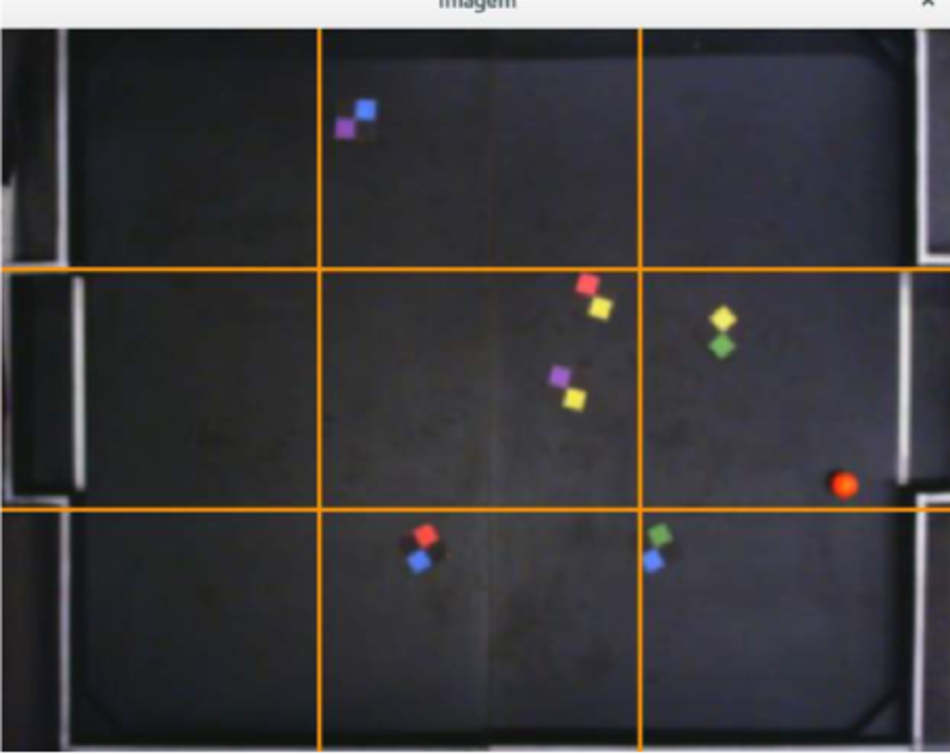
\includegraphics[width=0.4\textwidth]{vssvision.pdf} 	
%	\caption{Sistema de calibracao desenvolvido peloSIRLab \cite{Rosa:2015}}
%	\label{SIRLabCalibracao}
%\end{figure}
%O autor menciona que a calibração de cores e feita calibrando obrigatoriamente laranja, amarelo e azul, e então as outas cores referentes aos jogadores em campo. Como visto na Figura \ref{SIRLabCalibracao} a imagem da camera é dividida em nove cantos, e para calibrar a cor o usuario deve clicar em cima da cor que gostaria de ser calibrada salvando um intervalo de cor tratado como RGB máximo daquela cor e o mínimo, a medida
%que vão havendo os cliques o sistema verifica para cada atributo se ele é maior que o atributo
%máximo salvo ou menor que mínimo salvo, caso seja, o mesmo assume o lugar de menor ou
%maior\cite{Rosa:2015} e esse processo deve ser feito em cada um dos nove cantos da imagem. Os valores HSV encontrados sao ajustados manualmente com a ajuda de sliders, como visto na Figura \ref{SIRLabCalibracaoHSV}. Este processo de calibração pode demorar entre cinco e dez minutos.
%O desenvolvimento do sistema utiliza para procesamento de imagens a biblioteca OpenCV e para telas interativas a biblioteca  ImGui.
%
%\begin{figure}[!h]
%	\centering
%	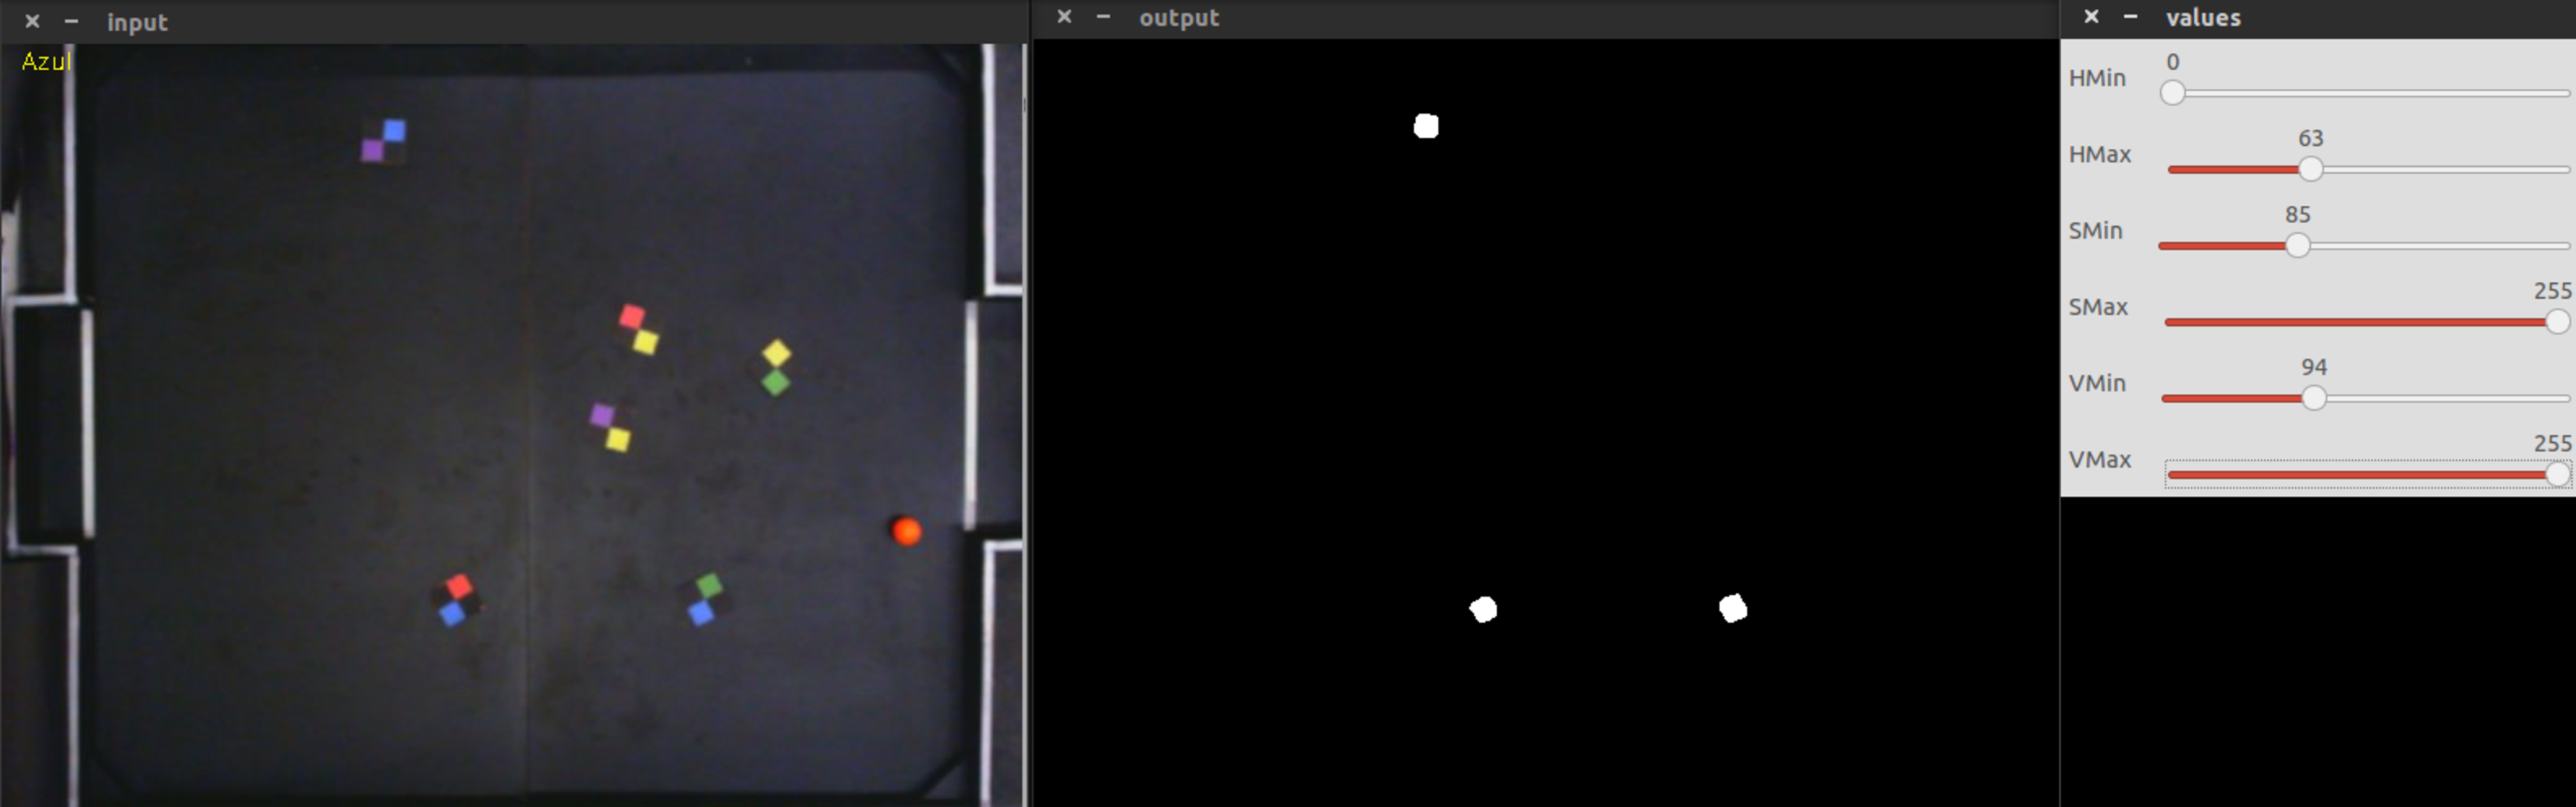
\includegraphics[width=0.8\textwidth]{calibration.pdf} 	
%	\caption{Sistema de calibracao desenvolvido peloSIRLab \cite{VSSVision}}
%	\label{SIRLabCalibracaoHSV}
%\end{figure}
%
%O atual sistema de visão computacional do SIRLab passou por algumas mudanças desde 2015 e conta com uma inteface e metodo de calibração diferentes\cite{VSSVision}. 
%Como disponivel no repositorio online do Laboratorio, o atual sistema de calibração de cores utiliza o espaço de cores HSV, no lugar do RGB\cite{Rosa:2015}. A antiga inteface do sistema, feita inicialmente em ImGui deu lugar à nova, desenvolvida em Qt, como mostrado na Figura \ref{SIRLabNova}.
%\begin{figure}[!h]
%	\centering
%	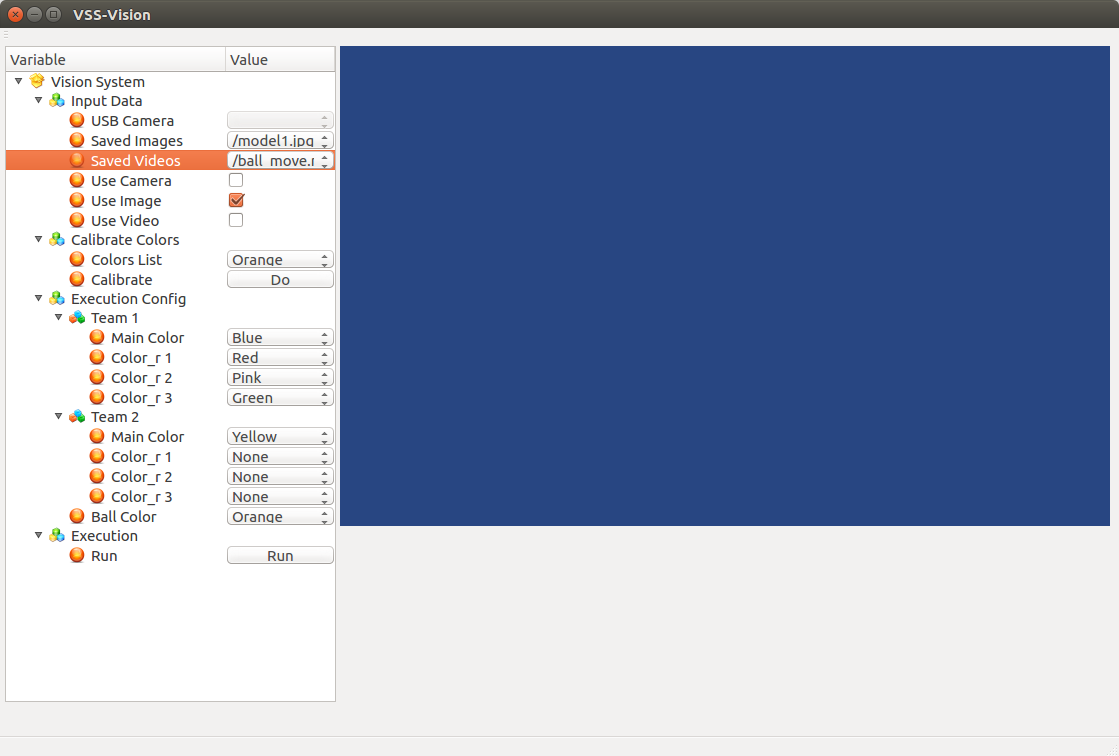
\includegraphics[width=0.5\textwidth]{vsssnovonormal.png} 	
%	\caption{Nova interface do time da SIRLab \cite{VSSVision}}
%	\label{SIRLabNova}
%\end{figure}
%
%O metodo de calibração de cores tambem foi modificado, segundo a equipe\cite{VSSVision} o sistema possibilita a calibragem de 8 cores, Laranja, Amarelo, Azul, Vermelho, Verde, Rosa, Roxo, Marrom. Após o usuário escolher uma cor para calibrar o mesmo deve encontrar um intervalo de cor, no espaço de cores HSV, que represente-a. Ao clicar na tela com o botão direito o sistema da um zoom na área para ajuste fino. A figura \ref{SIRLabNovaCalibracao} demonstra o novo metodo de calibração.
%
%\begin{figure}[!h]
%	\centering
%	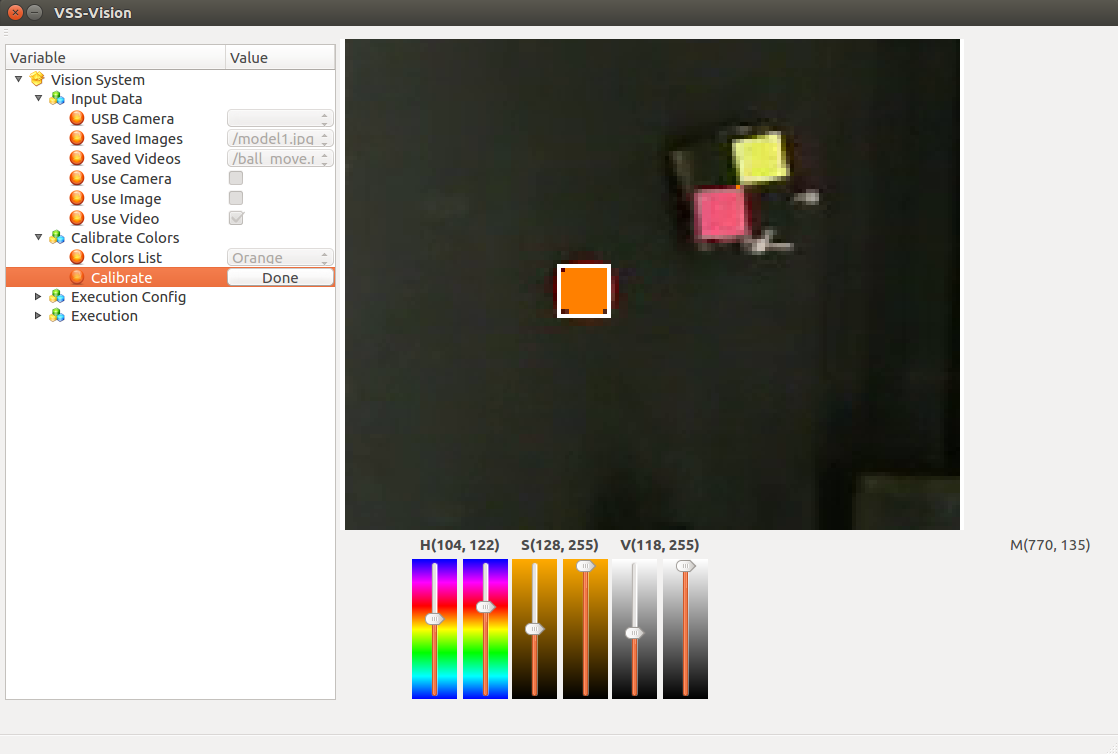
\includegraphics[width=0.5\textwidth]{vsssnovo.png} 	
%	\caption{Calibração atual do time da SIRLab \cite{VSSVision}}
%	\label{SIRLabNovaCalibracao}
%\end{figure}
 % Fundamentação
	%====================================================================================================
	% ?????
	%====================================================================================================
	% TCC
	%----------------------------------------------------------------------------------------------------
	% Autor				: Jasane Schio
	% Orientador		: Gedson Faria
	% Co-Orientador		: Angelo Darcy
	% Instituição 		: UFMS - Universidade Federal do Mato Grosso do Sul
	% Departamento		: CPCX - Sistema de Informação
	%----------------------------------------------------------------------------------------------------
	% Data de criação	: 01 de Outubro de 2015
	%====================================================================================================
	
	\definecolor{dkgreen}{rgb}{0,0.6,0}
	\definecolor{gray}{rgb}{0.5,0.5,0.5}
	\definecolor{mauve}{rgb}{0.58,0,0.82}
	
	\lstset{frame=tb,
		language=C++,
		aboveskip=3mm,
		belowskip=3mm,
		showstringspaces=false,
		columns=flexible,
		basicstyle={\small\ttfamily},
		numbers=none,
		numberstyle=\tiny\color{gray},
		keywordstyle=\color{blue},
		commentstyle=\color{dkgreen},
		stringstyle=\color{mauve},
		breaklines=true,
		breakatwhitespace=true,
		tabsize=3
	}
	\chapter{Metodologia e Desenvolvimento} \label{Cap:Processamento}
	
			Para o desenvolvimento foi escolhida a biblioteca OpenCV por ser OpenSource, multiplataforma, conter uma grande quantidade de métodos e algoritmos já implementados	e pelo seu rápido desempenho de máquina.
			A linguagem escolhida para o desenvolvimento foi o C++ pois é uma linguagem de programação compilada, o que torna sua execução mais rápida que as linguagem interpretadas, dando ao sistema grande desempenho, e por ser uma linguagem orientada objeto. 
			
			O sistema desenvolvido é separado em duas partes: Processamento e Interface Gráfica.
			A parte de Processamento é onde são feitas as partes de aquisição de imagem, processamento de imagem, conversão de imagem para modelo de cor HSV, seleção de pontos de cor e contagem de ocorrência de cor. Já a interface gráfica, é a onde ocorre a entrada do usuário para assim ser feita a calibração manual de mínimos e máximos de cada cor.
		
	
	Passos do projeto:
	\begin{description}
		\item[Aquisição de imagens em vídeo:] Nesse passo as imagem são adquiridas via câmera USB.
		
		\item[Identificação de Objetos:]
				 Durante o processo de aquisição de imagem são selecionados os objetos, quais serão usados como base para a detecção de máximos e mínimos de cores.
		\item [Cálculo de Mínimos e Máximos:]
		 Nessa etapa são levados em consideração os objetos teste. A imagem é "varrida"  por pixel na localidade dos objetos-teste e assim são salvos seus valores e feito a contagem de ocorrências de cada cor.		
	\end{description}


	\section{Projeto}
	\subsection{Organização do Projeto}
	 O projeto foi desenvolvido seguindo o paradigma de programação conhecido como  Orientação à Objetos, esse paradigma baseia-se na utilização de objetos individuais para criação de um sistema maior e complexo. A IDE usada para o desenvolvimento foi a QT Creator, esta separada o projeto em três pastas, Headers, Sources e Forms. Na pasta Headers estão os arquivos de cabeçalho(.h) onde estão as declarações dos métodos e variáveis usados nas classes  executáveis. Já na pasta Sources estão os arquivos fonte(.cpp), são nesses arquivos que os métodos declarados nos arquivos da pasta Header são implementados. Na pasta Forms está o arquivo de interface gráfica(.ui) que é usado no projeto para ser a ponte entre o usuario e as funções do sistema.
	 
	\begin{figure}[!h]
		\centering
		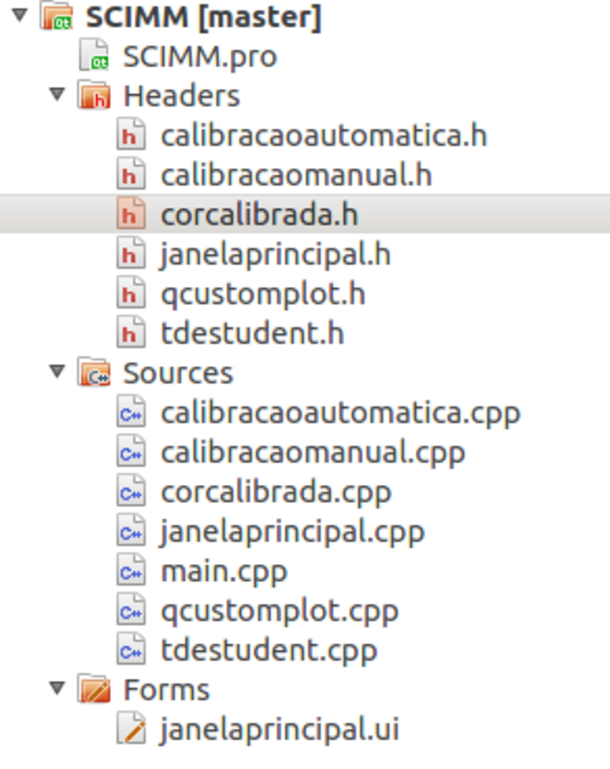
\includegraphics[width=0.2\textwidth]{organizacaoProjeto.pdf}
		\caption{Organização das pastas do projeto}
		\label{Organizacao do Projeto}
	\end{figure}
	Cada arquivo de cabeçalho possui um arquivo fonte correspondente, formando assim uma Classe, com exceção do arquivo fonte main, pois para este arquivo não há a necessidade.
	As classes desenvolvidas no projeto são:
 calibracao, manual, automatica, corcalibrada, janelaprincipal e tdestudent. Já a classe qcustomplot é um componente para auxilio em plotagem de gráficos e vizualização de dados\cite{QCustomPlot}.
Para melhor entendimento da interação entre as classes a figura 3.2 trás o diagrama de classes do projeto.
	 \begin{figure}[!h]
	 	\centering
	 	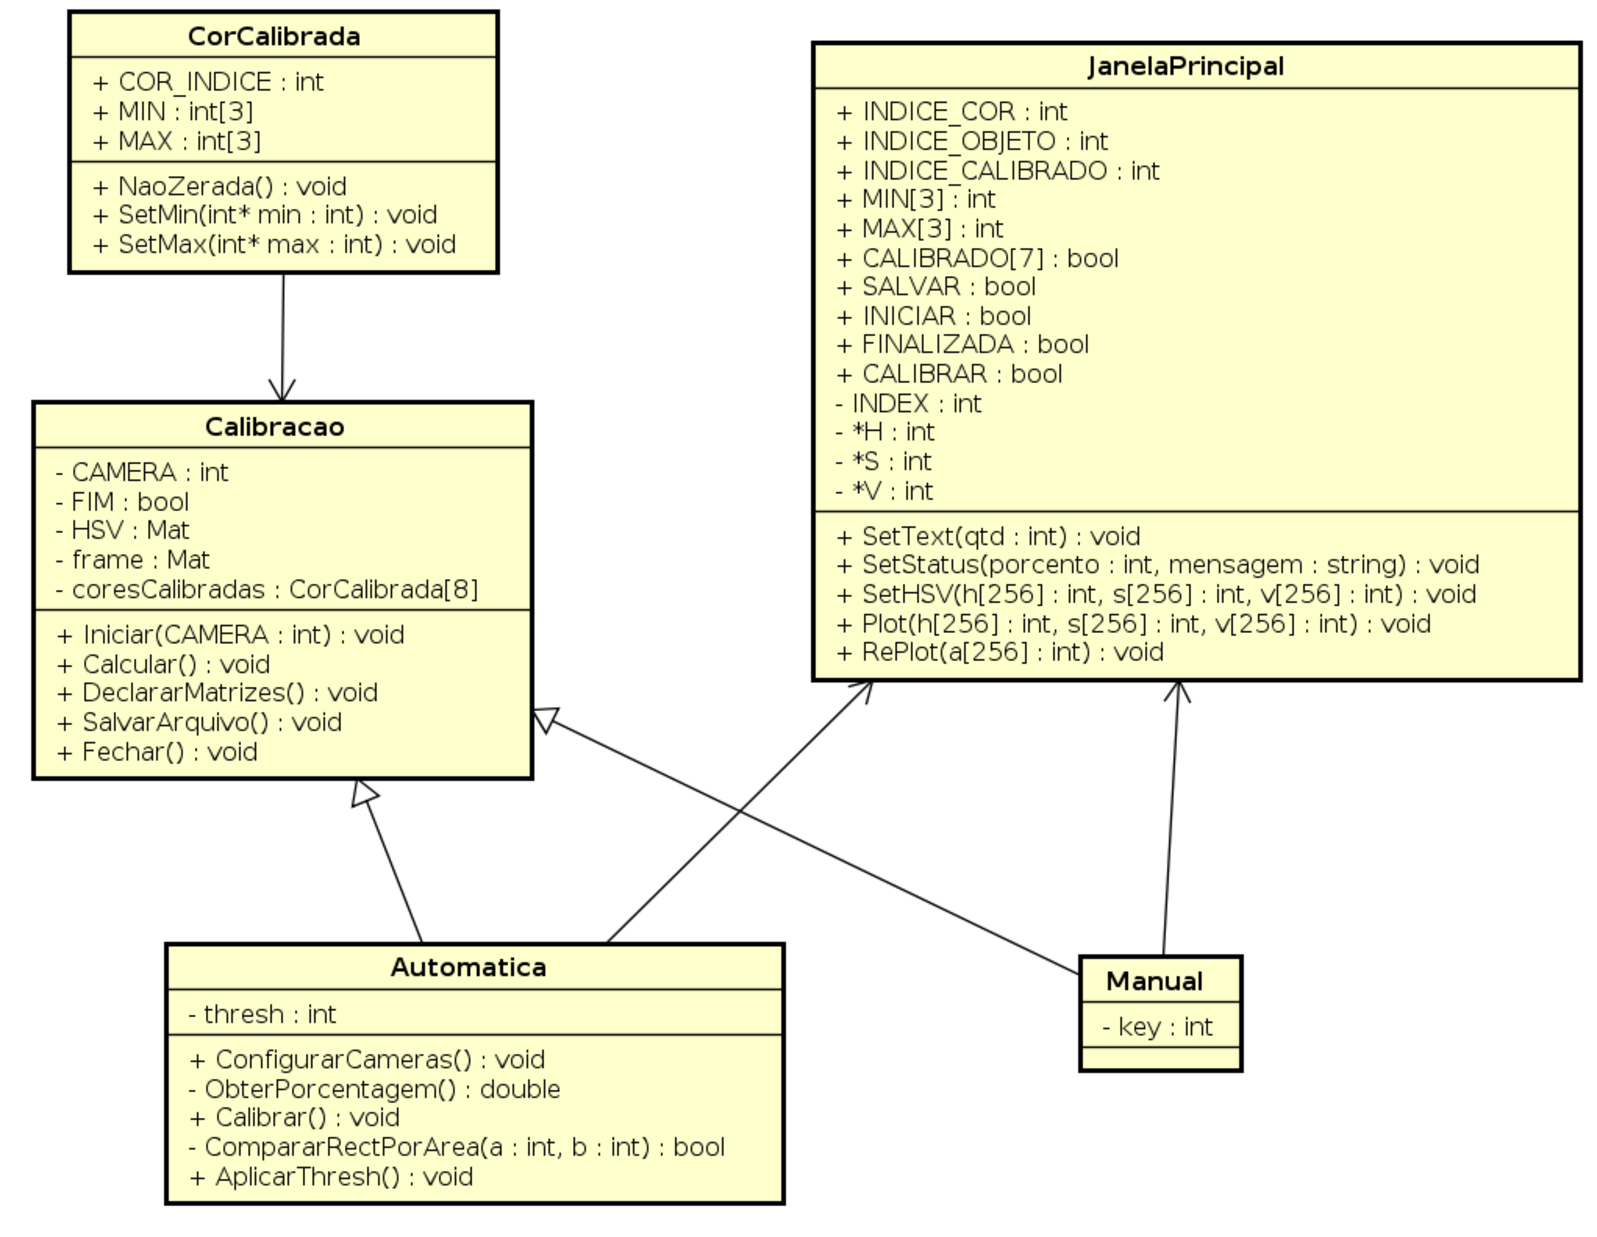
\includegraphics[width=0.8\textwidth]{diagramadeclasse.pdf}
	 	\caption{Diagrama de Classes do projeto}
	 	\label{DiagramaDeClasse}
	 \end{figure}\newpage


\subsection{Classes}
	\begin{description}

	\item [main] esta é a classe executavel do sistema, ela inicia o programa e em seguida chama a classe de interação grafica \textbf{janelaprincipal}  
	
	\item [janelaprincipal]	classe que faz a interação com o usuario e que de acorco com esta interação seleciona o tipo de calibração, e seus parametros, para então ser feita a analise dos pixeis	
		
	\item [calibracao] classe "pai" que contem os metodos e variaveis que virão a ser usadas por ambas as classes \textbf{manual} e \textbf{automatica}
	
	\item [manual] classe que contem os metodos, cálculo e variaveis necessarias para a calibração manual
	
	\item [automatica] classe que contem os metodos, cálculo e variaveis necessarias para a calibração automatica
			
	\item [corcalibrada] classe que salva o indice da cor já calibrada e seu intervalo de valores
	
	\item [tdestudent] esta é a classe que faz o cálculo probabilistico conhecido com TdeStudent
	

	\end{description}

	

	\section{Fluxo do Sistema}
O sistema possui um fluxo principal e dois subfluxos de acordo com o tipo de calibração escolhida. A Figura 3.3 mostra o fluxo principal do sistema.
		\begin{figure}[!h]
			\centering
			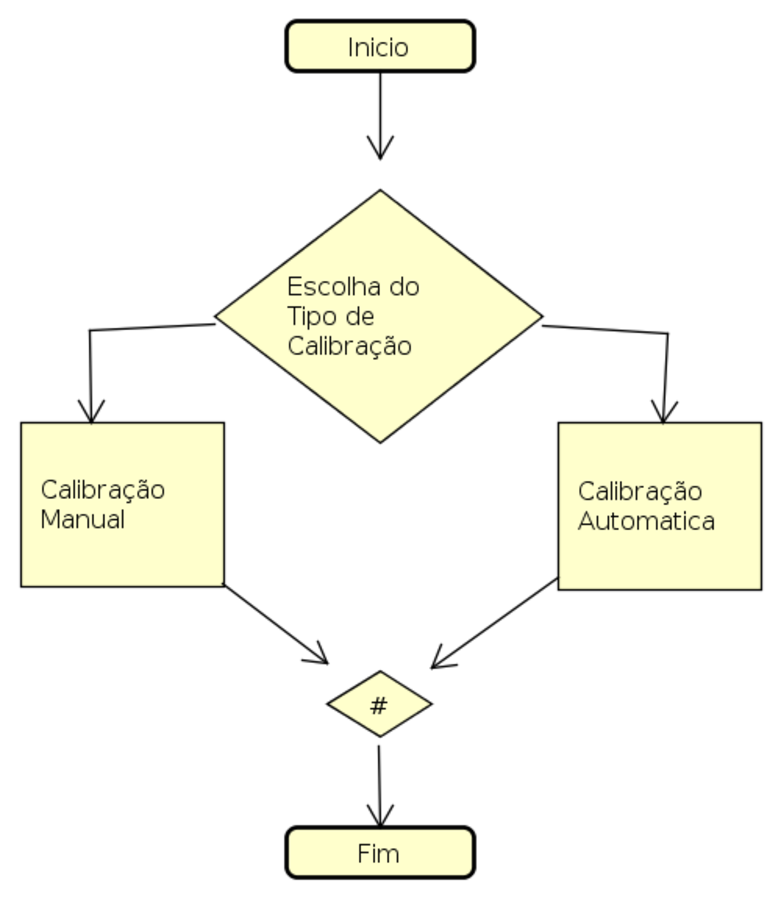
\includegraphics[width=0.45\textwidth]{fluxoprincipal.pdf}
			\caption{Diagrama de Fluxo}
			\label{FlowCHart}
		\end{figure} 
		
		 O fluxo principal do sistema consiste na apresentação da \textbf{interface grafica} ao usuario. A \textbf{interface grafica} por sua vez oferece as duas possibilidades de calibração: Calibração Manual e Calibração Automatica. De acordo com o tipo de calibração escolhido o sistema inicia um subfluxo. Apos a execução de todo subfluxo o sistema é finalizada.
			
	\subsection{Fluxo de Calibração Automatica}	
	O fluxo de calibração automatica possui o mínimo possivel de interação com o usuario. Neste fluxo o sistema faz automaticamente a detecção de objetos e utilizando a probabilidade matematica conhecida com T de Student verifica o tamanho de cada objeto encontrado para gerar um limite considerado o tamanho que os objetos que devem ser encontrados terão, nesse caso as etiquetas de cores dos robos e só então analisar os valores e calcular os valores mínimos e máximos de HSV automaticamente.	
	O fluxo inicia somente caso a camera esteja disponivel(1), apos a sua inicialização é feita a configuração da camera(2), enquadramento do tamanho correto e correção de brilho e luminosidade. Uma vez que a camera está configurada o sistema inicia a deteção de objetos e a validação dos objetos(3) que estão no tamanho correto. Apos deixar somente os objetos corretos no sistema, os pixeis de cada um são varridos e seu intervalo HSV encontrado(4). Os objetos e cores encontrados ficam disponiveis para o usuario apra esse fazer a assimilação entre os objetos e as cores corretas(5), após intervalos corretos já tiverem sido calibrados, um arquivo com os valores é gerado(6) e o usuario finaliza o sistema.
		\begin{figure}[!h]
				\centering
				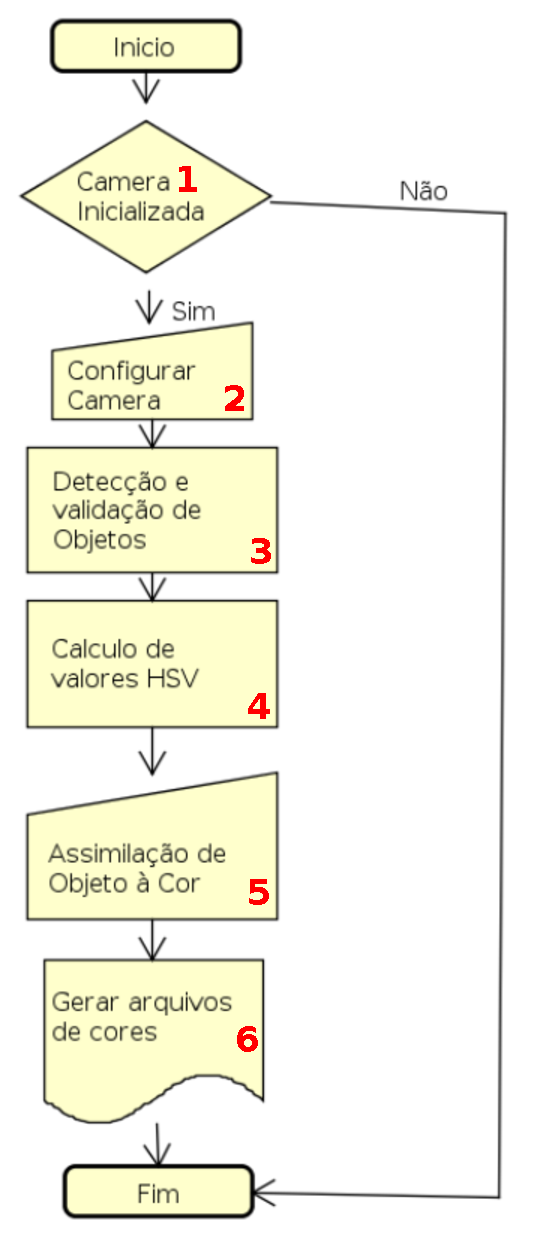
\includegraphics[width=0.45\textwidth]{fluxoautomatico.pdf}
				\caption{Diagrama de Fluxo Automatico}
				\label{DiagramaDeFluxoAutomatico}
			\end{figure} 
			
		Nas sessões à seguir explicarei detalhadamente cada processo da calibração automatica
	\subsubsection{Configuração de Camera}
Antes de ser feito o processo de calibração são necessarias duas configurações: Constrate e Brilho e o Recorte de Imagem.
A configuraça~o de contraste e brilho utiliza o metodo \textit{convertTo} da biblioteca \textit{OpenCV} e é utilizada para o melhoramento da imagem antes da detecção dos objetos, a utilização completa fica da seguinte maneira:
\begin{center}
\centering \textit{ frameA.convertTo(frameA, -1, contrast\_value / 50.0, brightness\_value)}
\end{center}
Esta função recebe quatro parametros. O primeiro \textbf{frameA} informa aonde sera salvo o resultado da conversão. O segundo \textbf{-1} indica o tipo da matrix, ou numero de canais, da imagem a ser gerada, usa-se -1 quando se deseja que se use os valores semelhantes aos da imagem da imagem original\cite{OpenCV}, O terceiro \textbf{contrast\_value / 50.0} indica o valor de constraste, ou alpha, a ser usado para multiplicar os valores do pixel da imagem\cite{OpenCV} e por ultimo \textbf{brightness\_value} que é o valor do brilho, ou beta, a ser adicionado à imagem. \newline
Outra configuração feita é o Recorte de Imagem, onde utilizando a função setMouseCallback para possibilitar a interção do usuario na imagem por meio do mouse, sua utilização é dada da seguinte maneira:
\begin{center}
\centering \textit{ cv::setMouseCallback(src\_window,mouseHandler,0);}
\end{center}
Tem como primeiro parametro \textbf{src\_windows} que indica a janela na qual a função recebera a interação,  o segundo, \textbf{mouseHandler}, indica a função na qual esta implementada a interação e o ultimo parametro, \textbf{0}, indica parametros opcionais, neste caso não usaremos nenhum então foi usado o numero 0.
Dentro da função \textbf{mouseHandler} são identificados os pontos iniciai e final da seleção na tela e utilizada a função \textit{rectangle} para demarcar a seleção na tela. A utilização da função \textit{rectangle} completa fica da seguinte maneira:
\begin{center}
\centering \textit{ cv::rectangle(frameA, point1, point2, CV\_RGB(255, 0, 0), 2, 5, 0);}
\end{center}
A função rebece os parametros \textbf{frameA} indicando a imagem na qual será demarcada a area selecionada, depois o parametro \textbf{point1} que é o ponto incial de seleção na imagem, \textbf{point2} que é o ponto final da seleção. \textbf{CV\_RGB(255, 0, 0)} que indica a cor da demarcação, \textbf{2} indicando a expessura da demarcação, \textbf{5} que significa o tipo de linha a ser utilizado na demarcação e \textbf{0} que é o numero de bits fracinarios.
 Após confirmada a escolha do tamanho da tela 
este é então salvo na variavel nomeada \textit{tamanho}, está então sera usado durante todo o processo de calibração.
\newpage
\subsubsection{Detecção e validação de Objetos}
A detecção dos objetos a serem calibrados é dada pelo algoritmo de detecção de bordas de Canny. Como mais um recurso para eliminação de ruidos e melhoria da imagem antes de ser executado a detecção de objetos atravez da detecção de bordas é utilizado desfoque na imagem. O algoritmo de Canny já está implementado dentro da biblioteca OpenCV e com a seguite usagem:
\begin{center}
\centering \textit{  Canny(src\_gray, canny\_output, thresh, thresh * 3, 3);}
\end{center}
O algoritmo de Canny utiliza por padrão imagem em padrões de cinza, sendo assim \textbf{src\_gray} é a imagem orignal tranformada para escala de cinza, esta é a imagem na qual o algoritmo sera aplicado. \textbf{canny\_output} será a imagem de saida da função.
\textbf{thresh} e \textbf{thresh*3} são os limites mínimos e máximos para considerar uma borda. \textbf{3} é o valor de apertura ou kernel, o valor 3 é utilizado como padro.

Apos o uso do algoritmo de Canny para detecção de bordas é necessario então fazer uso da função \textit{findContours}, nativa no \textit{OpenCV} para detecção de contornos.
\begin{center}
\centering \textit{ findContours(canny\_output, contours, hierarchy, CV\_RETR\_EXTERNAL, CV\_CHAIN\_APPROX\_SIMPLE, Point(0, 0))}
\end{center}

O primeiro parametro, \textbf{canny\_output}, é a imagem que o algoritmo de Canny gerou com as bordas encontrada na imagem, e é a imagem que o método \textit{findContours} ira utilizar para detectar os contornos, \textbf{contours} é o parametro que indica onde serão salvos os contornos encontrados, cada contorno é armazenado como sendo um vetor de pontos \cite{OpenCV}. \textbf{hierarchy} é onde será salva um verot de informações sobre a topologia da imagem, e terá como total de elementos o mesmo numero que o total de contornos encontrado\cite{OpenCV}. O quarto parametro, \textbf{CV\_RETR\_EXTERNAL} indica o modo de obtenção de contornos, nesse caso \textit{CV\_RETR\_EXTERNAL} indica que o metodo só obtera os contornos exteriores\cite{OpenCV}. \textbf{CV\_CHAIN\_APPROX\_SIMPLE} indica o metodo que sera usado para aproximação de contornos, o metodo \textit{CV\_CHAIN\_APPROX\_SIMPLE} comprime segmentos horizontais, verticais, diagonais e deixa apenas os seus pontos finais\cite{OpenCV}. E o ultimo parametro, \textbf{Point(0, 0)}, indica o valor a ser usado para deslocar a imagem ao encontrar os objetos, neste caso esse valor é 0 para Y e 0 para X, pois não sera necessario. 

Uma vez obtidos os contornos é necessarios que se faça a eliminação de vertices dos polignos encontrados nos objetos deixando assim o objeto mais preciso. Isso é necessario para deixar a forma encontrada mais precisa dá forma original. Para este ajuste foi usado o metodo \textit{approxPolyDP}, ja implementado dentro da biblioteca OpenCV. Esse metodo teve que ser aplicado em cada um dos contornos encontrados, e foi utilizado da seguinte maneira:
\begin{center}
\centering \textit{    approxPolyDP(Mat(contours[i]), contours\_poly[i], 3, true)}
\end{center}
 Onde o metodo inicia recebendo como paralametro, \textbf{Mat(contours[i])} que é a criação de uma nova imagem, somente com aquele unico objeto, que esta sendo analisado. A seguir é informado no segundo parametro a variavel de destino \textbf{contours\_poly[i]}, onde sera salvo o objeto com a eliminação dos vertices. O terceiro parametro indica o valor do \textit{epilson}, usado o valor \textbf{3} que especifica a precisão da aproximação, a distância máxima entre a curva original e a sua aproximação\cite{OpenCV}. O ultimo parametro indica se a curva aparoximada sera fechada ou não, foi usado o valor \textbf{true} pois neste caso fechar um uma curva é necessario para que o objeto onde está a cor, seja idenficado e analisado na probabilidade.
 
 Por ultimo os objetos possuem sua borda ignorada, sendo assim calculado o tamanho interior dele, para que por ventura não hajam pixeis de cor preta ou derivadas a serem calculadas.
 
 A detecção de contorno detecta todos os contornos possiveis na imagem, isso inclue sombras, luzes entre outras coisas. Mas não são todos os objetos encontrados que deverão ser calculados, sendo assim foi usado o cálculo probabilistico T de Student.
 Foi implementado uma biblioteca para o uso da probabilidade voltada para objetos Rect, os objetos da biblioteca \textbf{OpenCV} obtidos na detecção. Essa biblioteca analisa a lista de objetos encontrados na detecção e faz o cálculo dos limites, tamanho mínimo e máximo, dos objetos. Apos a obtenção desse limite pela biblioteca são analisados todos os objetos encontrados na detecção e os cujo tamanho não esteja dentro deste limite são removidos da lista.
 
 \subsubsection{Calculo de valores HSV}
 Para que possam ser feitos os cálculo de valores HSV mínimo e máximos é necessario que se faça, primeiramente a conversão da imagem obtida pela camera, normalmente no espaço de cores RGB, para o espaço de cores HSV, pois a mesma lida melhor com deferenças de luminosidade. 
 A biblioteca \textbf{OpenCV} converte o espaço de cor usando a função \textit{cvtColor} que utiliza da imagem original, e de uma imagem vazia com memoria alocada para ser salva a imagem apos a conversão, além do parametro do tipo de conversão, Exemplo do uso do método:
\begin{center}
\centering \textit{cvtColor(frame, HSV, CV\_RGB2HSV);}
\end{center}

Apos a conversão é necessario, então, ser feita uma analise dos objetos encontrados. Para cada objeto serão somadas as ocorrencias de cada um dos valores, HSV, e salvos separadamente em um vetor para cada, H, S e V com 256 posiçoes, uma vez que se sabe que os valores de um pixel varial de 0 a 255. As ocorrençias são salvas se baseando no valor HSV do pixel. Para isso o pixel é separado em valores H, S e V este então tera seu valor correspondente a posição no vetor apropiado, por exemplo, se o valor de H em um determinado pixel for de 87, a posição de numero 87 no vetor ganhara uma ocorrencia a mais. No codigo, fica da seguinte maneira.
		\begin{lstlisting}
for (int y = insideRect.at(i).tl().y; y < insideRect.at(i).br().y; y++) {
 for (int x = insideRect.at(i).tl().x; x < insideRect.at(i).br().x; x++) {
	                pixel = HSV.at<cv::Vec3b>(y, x);
	                H[pixel.val[0]]++;
	                S[pixel.val[1]]++;
	                V[pixel.val[2]]++;
	            }
	        }	\end{lstlisting}

Uma vez terminada a analise dos pixeis do objeto o sistema procupa o valor mínimo e máximo, ou seja a primeira e ultima ocorrencia. Esses valores são encontrados procurando o primeiro valor de pixel que não esta zerado e o ultimo valor que não esta zerado. Isto é feito para eliminar que durante a analise o numero de valores a serem comparados ao valor real do pixel, da imagem final, seja menor. Para exemplificar a Figura 3.6 tras o gráfico dos valores de H da calibração de um certo objeto antes de ser feia a eliminação dos valores. Se fosse analisado esses valores, não eliminando os valores zerados, o sistema buscaria no valor de H do pixel desde o valor 1 ao 126 sem a necessidade, pois se não houve ocorrencia desses valores no objeto de referencia, o que foi analisado, então esses valores não fazem parte da cor desejada.
% e tambem para remover ruidos de outros cores para que estas não interfiram na pureza da busca da dada cor.

\begin{figure}[!h]
	\centering
	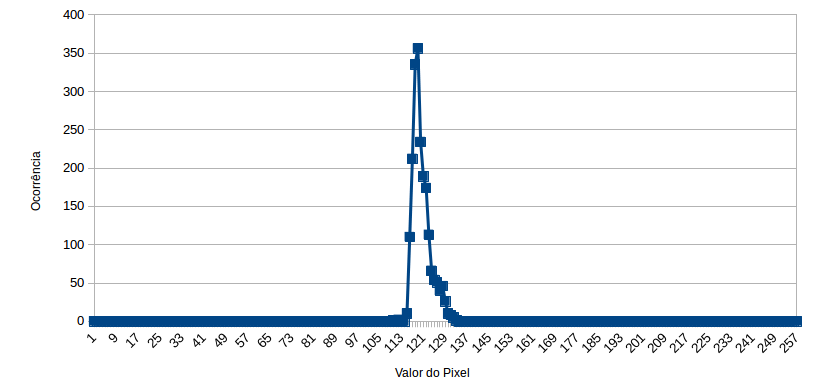
\includegraphics[width=0.5\textwidth]{graficototal.png}
	\caption{Grafico Exemplificando a Ocorrencia dos valores de H.}
	\label{Grafico Exemplo}
\end{figure}

 Apos ser feita a eliminação, Figura 3.7, de valos sabemos que somente a partir do pixel 110 houve ocorrencia, assim quando for necessario analisar pixel a pixel, os valores abaixo de 110 serão ignorados, ou seja não fazem parte da cor desejada.
 \begin{figure}[!h]
 	\centering
 	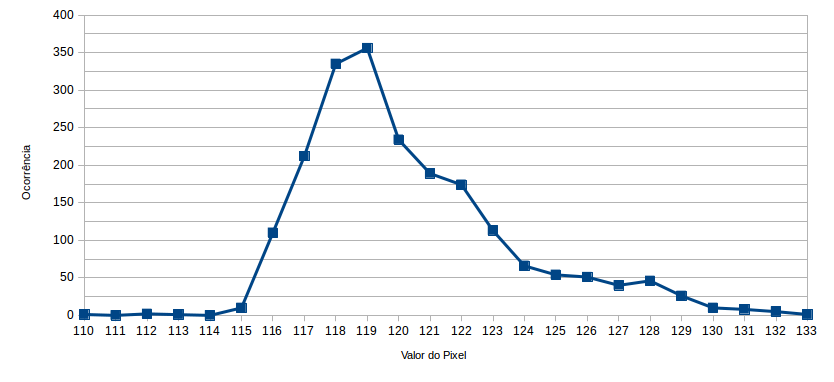
\includegraphics[width=0.5\textwidth]{graficominmax.png}
 	\caption{Grafico Exemplificando a Ocorrencia dos valores de H após eliminação.}
 	\label{Grafico Exemplo}
 \end{figure}

Após serem encontrados os valores mínimo e máximos para H, S e V de cada objeto detectado, estes valores são salvos em uma lista de objetos do tipo CorCalibrada. Neste objeto são salvos os respectivos valores.

 \subsubsection{Assimilação de Objeto à Cor}
 Uma vez que os objetos já foram identificados, suas cores analisadas e gerada sua lista. O sistema, utilizando do recurso de interface gráfica disponivel pela biblioteca Qt, informa ao usuario uma lista com os intervalos de cores encontrados, e outra lista com as possiveis cores a serem assimiladas para eles. Assim o usuario pode analisar um por um dos objetos e escolher qual se assemelha a qual cor. Assim que assimilada a cor ao objeto este é salvo e seu objeto CorCalibrada na lista de objetos salva o valor da cor em seu atributo COR\_INDICE.
 
  \subsubsection{Gerar Arquivo de Cores}
  Assim que todas as cores já estiverem sido assimiladas e a calibração finalizada, gera-se um arquivo chamado \textbf{cores.arff} contendo o indice de cada cor calibraa e seus valores máximos e mínimos.
  
  		
  	\subsection{Fluxo de Calibração Manual}	
   	O fluxo de calibração manual é iniciado somente se a camera estiver disponivel. Após a camera ser inicializada(1) o sistema espera pela seleção do objeto(2) o qual tera seus pixeis calculados para gerar os valores HSV. Com o objeto selecionado o usuario escolhe então a cor(4), na opção de escolha de cor, e calibrar. A area selecionada é então analisada e os valores de cada pixel calculados analisando seu HSV(3).
   	O usuario então seleciona os valores que considera satisfatorios(5). Enquanto houverem objetos a serem calibrados(6) o sistema repete esta mesma rotina, quando todos os objetos já tiverem sido calibrados, um arquivo com os valores é gerado(7) e o usuario finaliza o sistema.
  		\begin{figure}[!h]
  				\centering
  				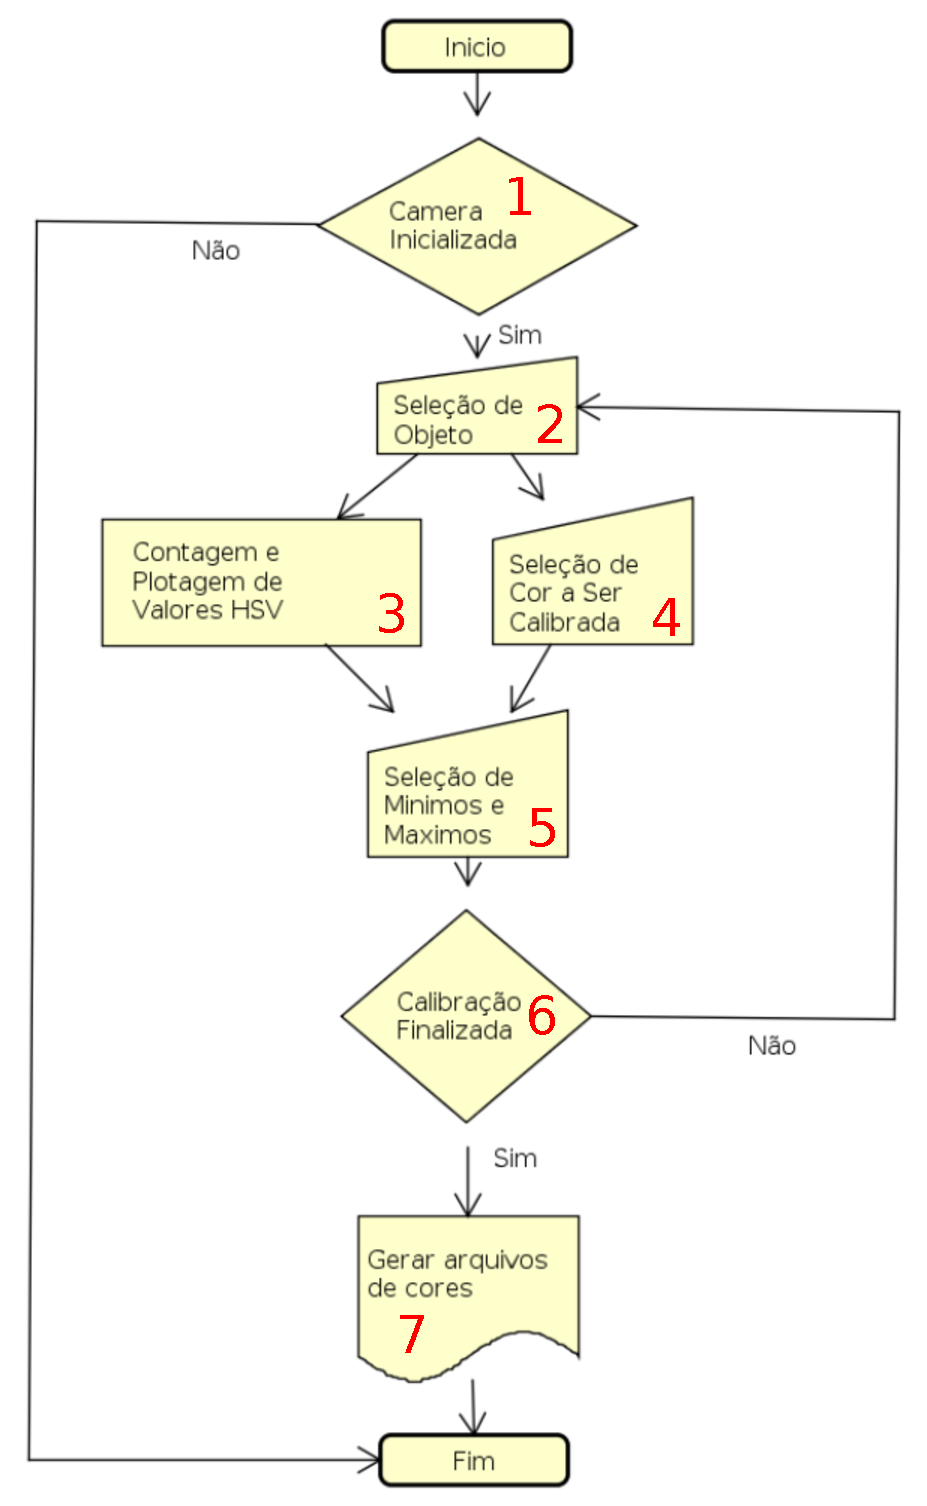
\includegraphics[width=0.45\textwidth]{fluxomanual.pdf}
  				\caption{Diagrama de Fluxo Manual}
  				\label{DiagramaDeFluxoManual}
  			\end{figure}
  			
  	\subsubsection{Seleção de Objeto}	
  	O primeiro passo para ser feita a calibração manual é a seleção de Objeto. Com o auxilio da função setMouseCallback, disponivel na biblioteca \textbf{OpenCV} e já explanada na sessão 3.2.1, é possivel obter os pontos de uma seleção feita na imagem, seu uso é necessario, já que obtenção de um ou mais objetos com a \textbf{mesma cor} a serem analisados é feita somente com a interação do usuario. Neste seleção existe a possibilidade de escolher somente um objeto ou mais de um objeto da mesma cor em diferentes pontos do campo, a seleção é feita somente um objeto por vez e cada objeto é analisado e seu valor e ocorrencia calculado utilizando o mesmo metodo encontrado na sessão 3.2.1 subsessão \textbf{Calculo de valores HSV}, estes valores são armazenados em memoria de execução e somente mostrados ao usuario quando requisitados. 
  	
  	\subsubsection{Plotagem de Valores HSV}	
  	Uma vez que o usuario já selecionou todos os objetos e os mesmos já foram analisados, o processo de calibração encaminha à interface grafica os valores encontrados e está plota três gráficos, um para cada um dos valores HSV.
  	Com a ajuda do componente auxiliar qcustomplot os gráficos são mostrados no sistema informando para o usuario quais foram os valores obtidos na seleção.
  	
  	\subsubsection{Seleção de Cor a ser Calibrada}
  	A seleção da cor na lista de cores possiveis para ser assimilado, pode ser considerada uma ação concomitante à ação de plotagem de graficos sendo que uma não depende dá outra, já que no momento da seleção do objeto o usuario já tinha em mente qual era sua cor, e a plotagem do gráfico não interfere nessa escolha, já a plotagem do gráfico é uma ação somente visual e não tem influencia da cor escolhida.
  	
  	\subsubsection{Seleção de Minimos e Maximos}
  	 Assim que os graficos são plotados, se torna então possivel, utilizando o recurso Slider, de fazer a seleção dos valores, tanto mínimo, quanto máximo. Ao ser modificado, cada um dos valores, o gráfico se ajusta para melhor detalhar ao usuario a ocorrencia dos pixeis. Ao contrario do sistema automatico, no sistema manual o objeto CorCalibrada só é criado após a seleção da cor e dos intervalos pelo usuario. Quando este salva a cor na interface gráfica, a mesma cor é encaminhada para o sistema manual e assim salva na lista.
  	 
  	 
\subsubsection{Gerar Arquivo de Cores}
Do mesmo modo que ocorre na calibração automatica, uma vez que todas as cores já estiverem sido assimiladas pelo usuario, este então finaliza a calibração e um arquivo com os valores calibrados é salvo localmente.
  	   	
  		
  	
%====================================================================================================
% ?????
%====================================================================================================
% TCC
%----------------------------------------------------------------------------------------------------
% Autor				: Jasane Schio
% Orientador		: Gedson Faria
% Co-Orientador		: Angelo Darcy
% Instituição 		: UFMS - Universidade Federal do Mato Grosso do Sul
% Departamento		: CPCX - Sistema de Informação
%----------------------------------------------------------------------------------------------------
% Data de criação	: 01 de Outubro de 2015
%====================================================================================================

\chapter{Aplicativo} \label{Cap:Aplicativo}
\section{Tela Principal}
\begin{figure}[!h]
	\centering
	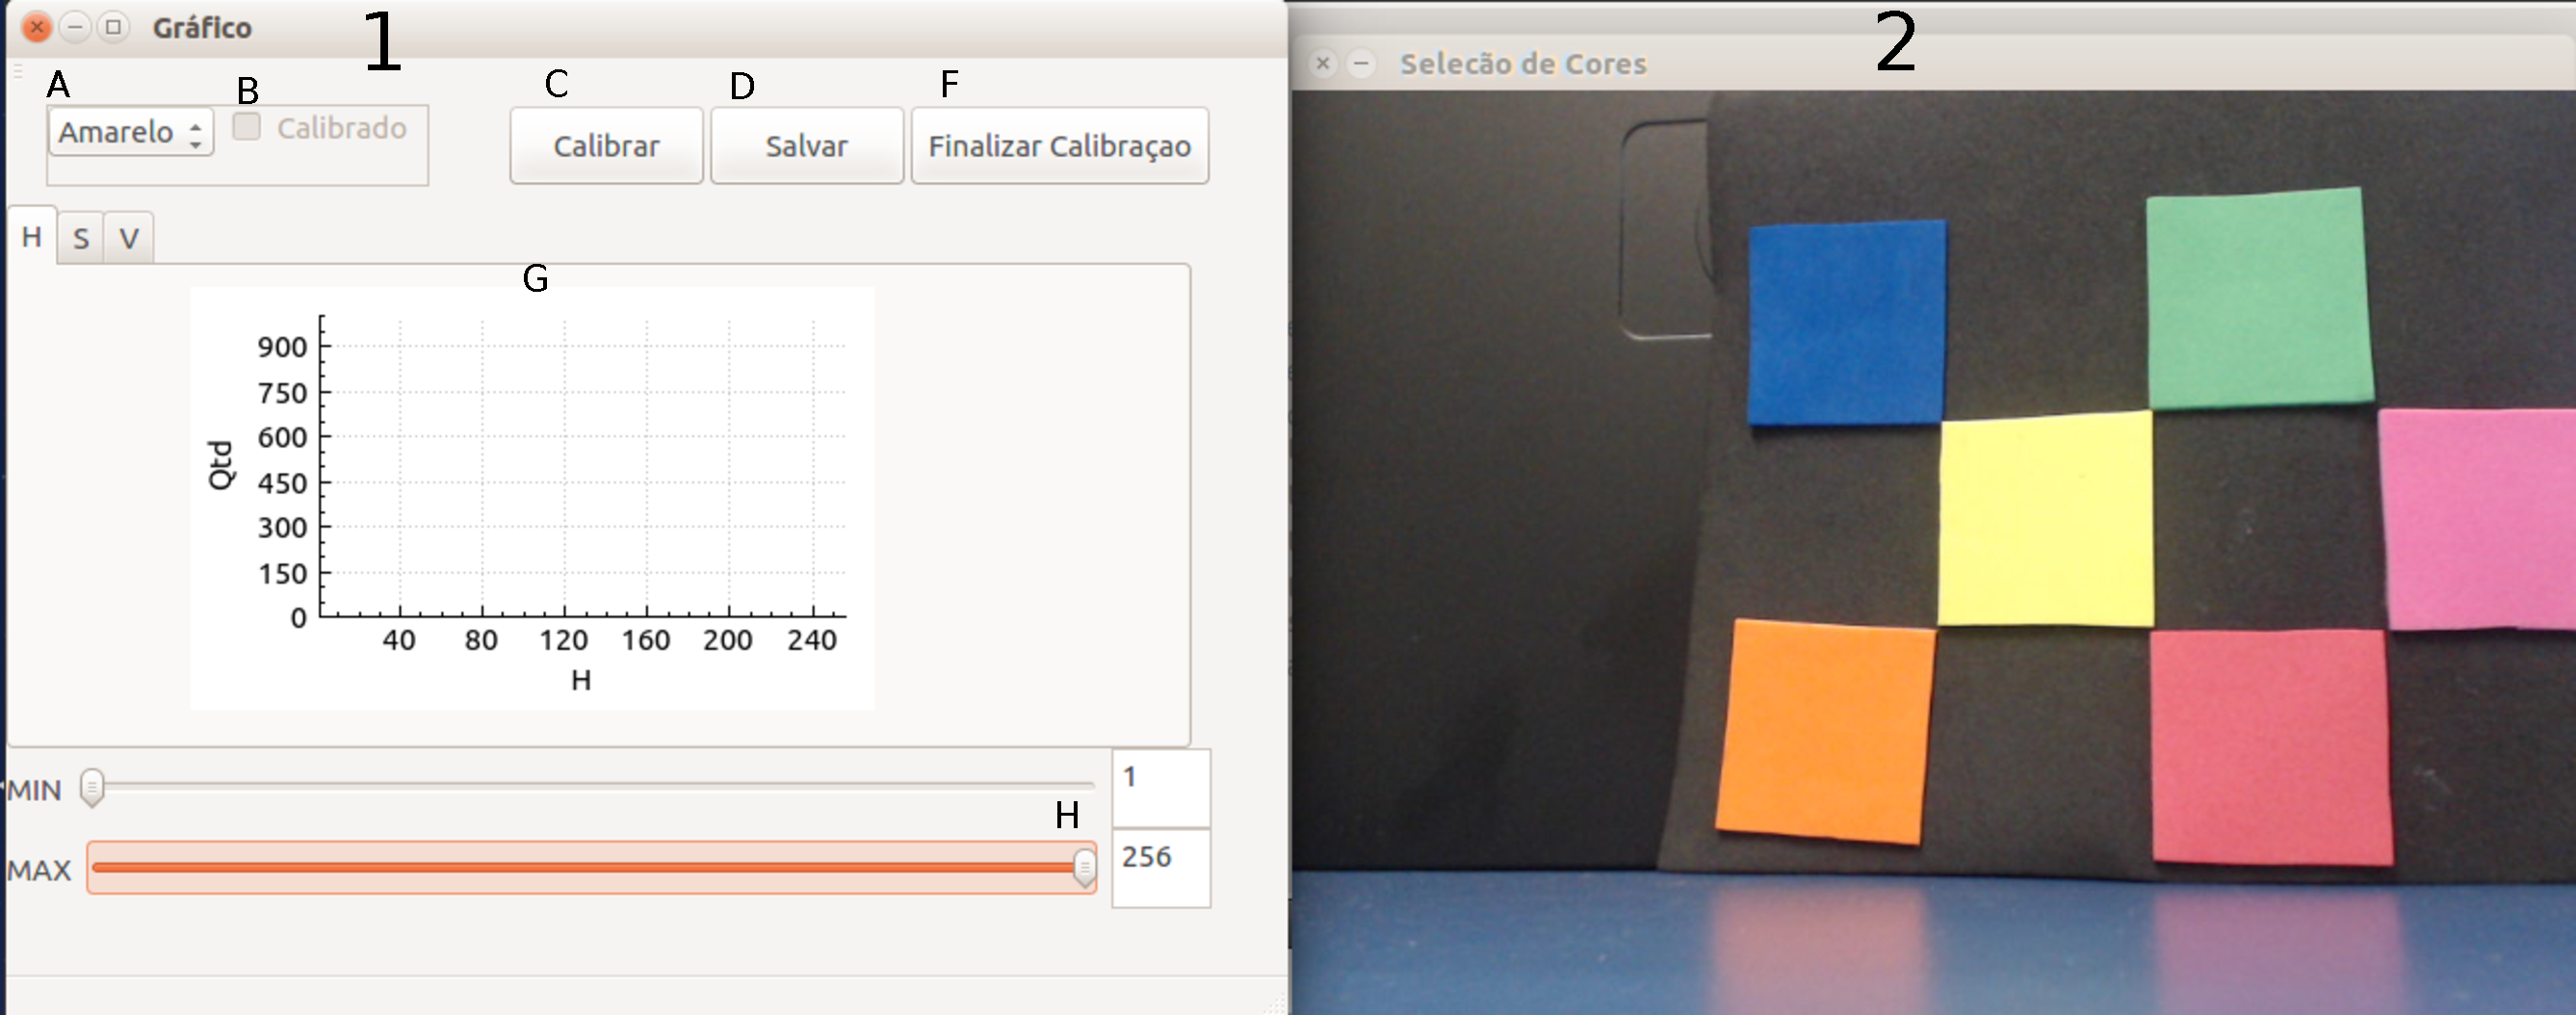
\includegraphics[width=0.98\textwidth]{manual1.pdf}
	(a) Janela 1 \hspace{5cm} (b) Janela 2
	\caption{Janelas do Sistema: Janela 1 e Janela 2 }
	\label{TelanInicial}
\end{figure}
A tela do sistema é formada por duas janelas. Janela 1 é a janela que recebe as interação do usuário, a Janela 2 é composta pela imagem obtida pela câmera, e para ser feita a escolha da cor.
Na Janela 1 possui ações de escolha de cor via Combo Box(A), um Check Box(B) que informa se a cor já foi calibrado ou não. Botões de Calibrar(C), que é usado apos a seleção da cor para a geração do gráfico, Salvar(D), que é usado apos a seleção dos valores para que estes sejam salvos na memoria do aplicativo, e Finalizar Calibração(F) que ira salvar os valores em arquivo. Uma área de gráfico (G) onde são mostrados os valores de ocorrência de H, S e V, cada um em uma aba diferente. A Janela 1 ainda possui um área de seleção dos valores(H), com região MIN e MAX que possui tanto Sliders quando Área de texto para seleção dos valores mínimos e máximos.
 \newpage

\section{Seleção do Objeto Colorido}
\begin{figure}[!h]
	\centering
	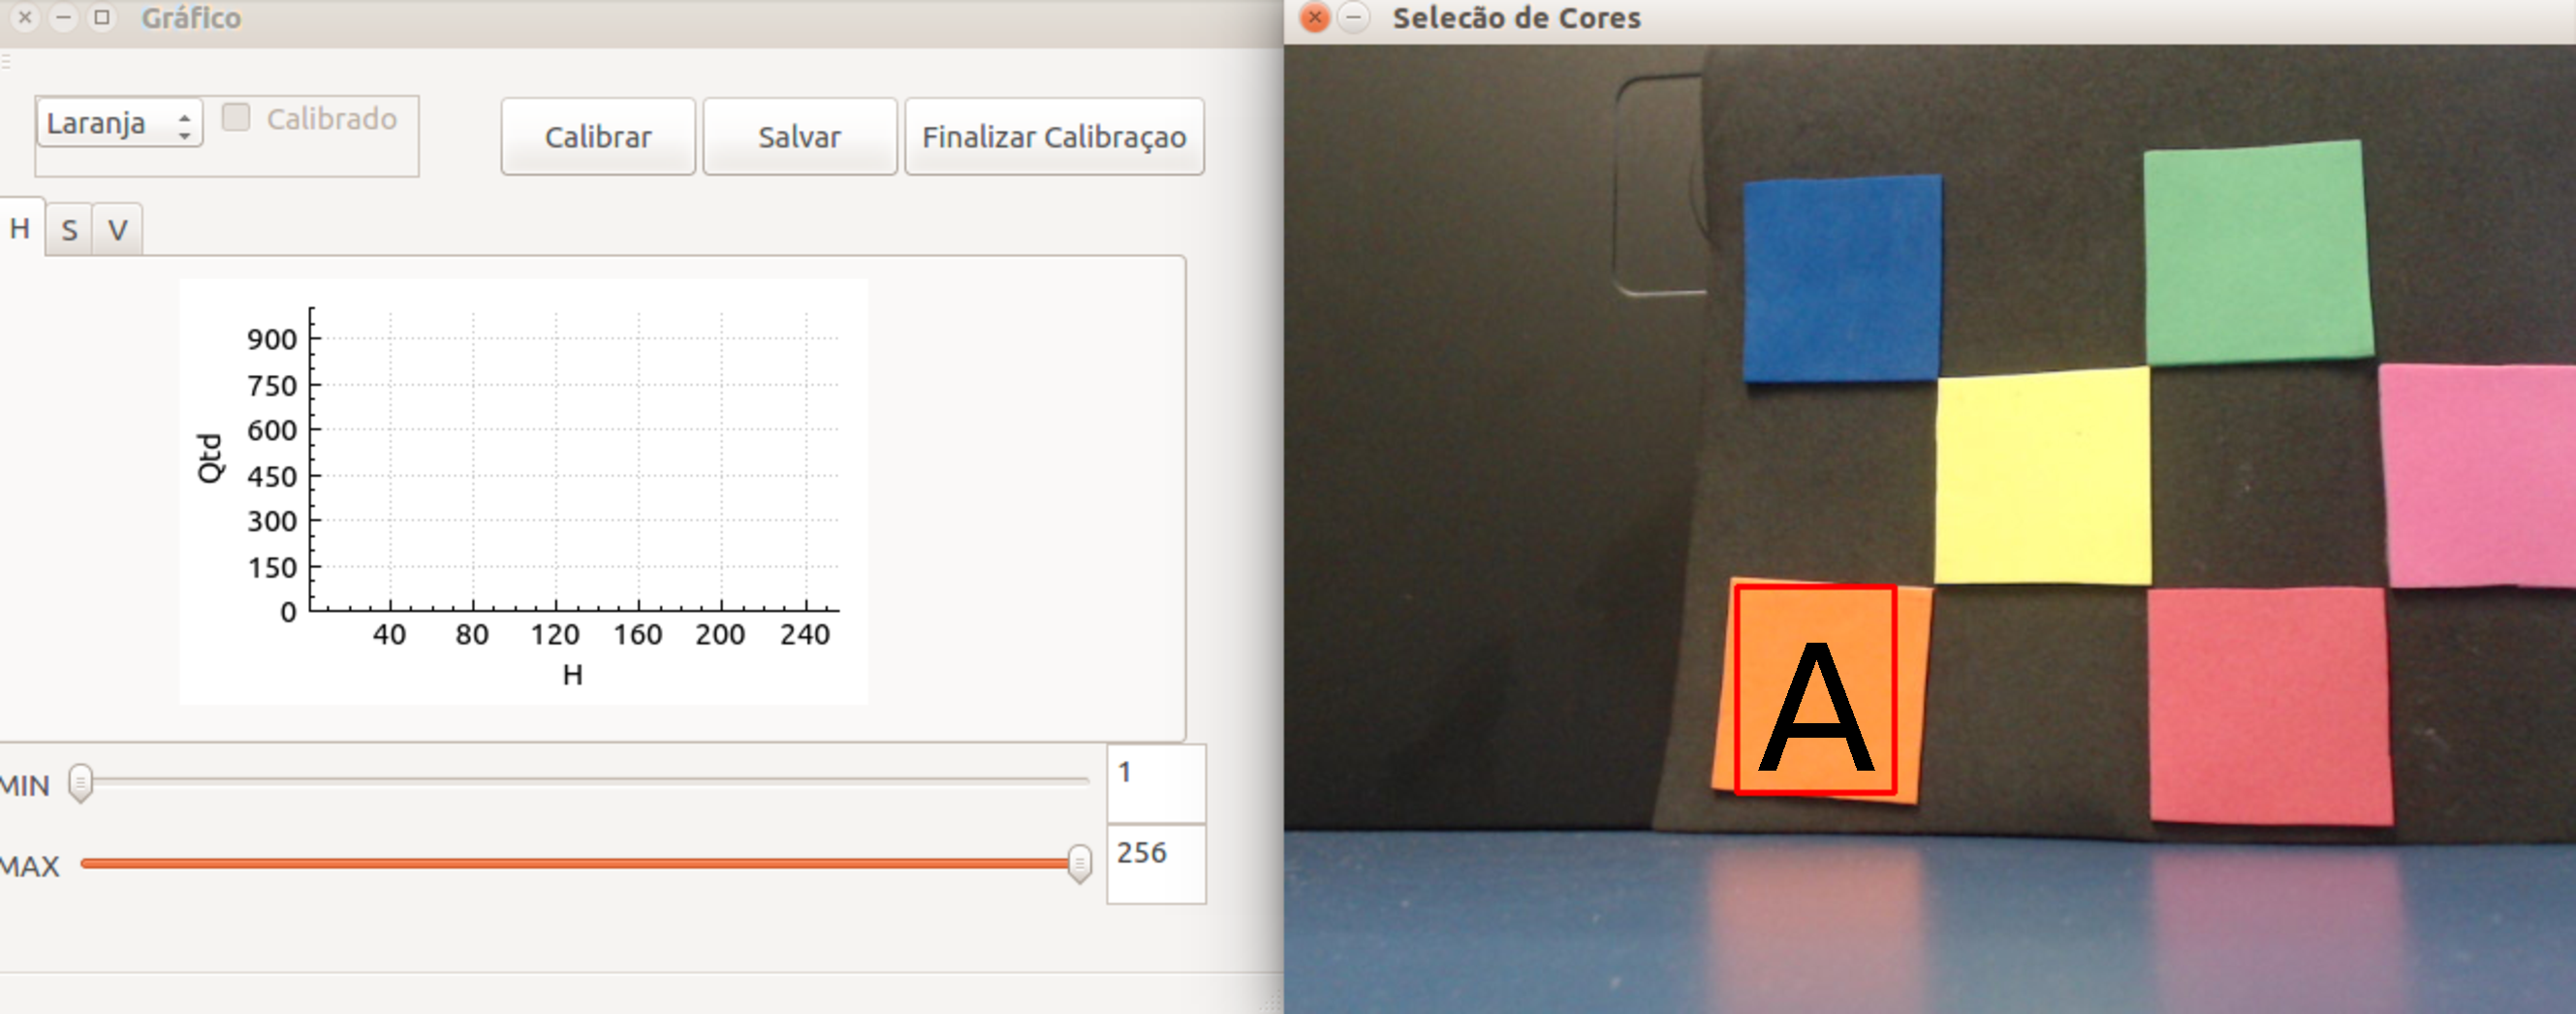
\includegraphics[width=0.98\textwidth]{manual2.pdf}
	\caption{A seleção do ponto com a cor, é obtido pela interação do usuário.}
	\label{SelecaoCor}
\end{figure}
A seleção das cores é feita selecionando, com o ponteiro do mouse clicando na área inicial e arrastando até a área final do objeto correspondente a cor. Um exemplo de seleção de cor ocorre na Figura 4.2 em A onde é selecionada a cor Laranja. Apos seleção da cor é necessário apertar no botão Calibrar para assim ser feito os cálculos dos valores HSV dos pixels e ser gerado o gráfico.

\section{Geração de Gráfico}
\begin{figure}[!h]
	\centering
	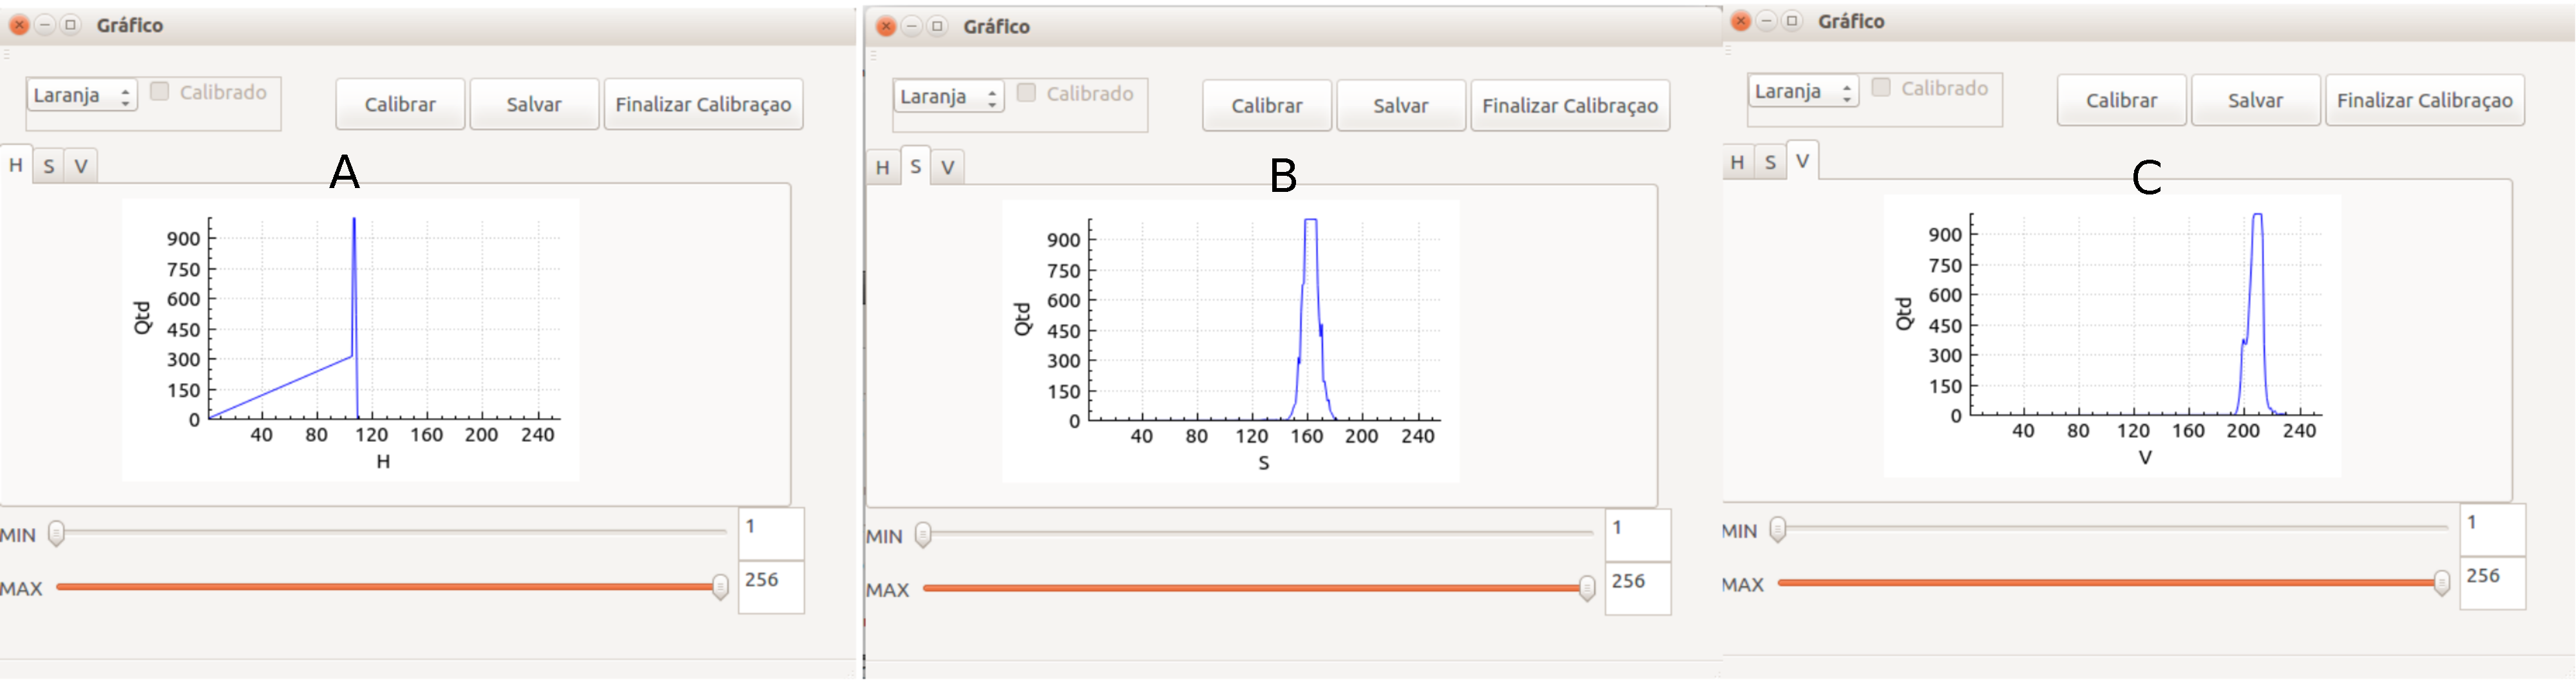
\includegraphics[width=0.98\textwidth]{manual3.pdf}
	\caption{Gráfico gerado após seleção dos pontos de cor.}
	\label{GraficoGerado}
\end{figure} 
Quando se aperta o botão Calibrar são gerados os 3 Gráficos de ocorrência de valor de H(A), S(B) e V(C), um em cada aba. No gráfico são vistos quais os valores que possuem mais ocorrência, para assim ser feita a seleção.
\newpage
\section{Seleção de Minimos e Maximos}
\begin{figure}[!h]
	\centering
	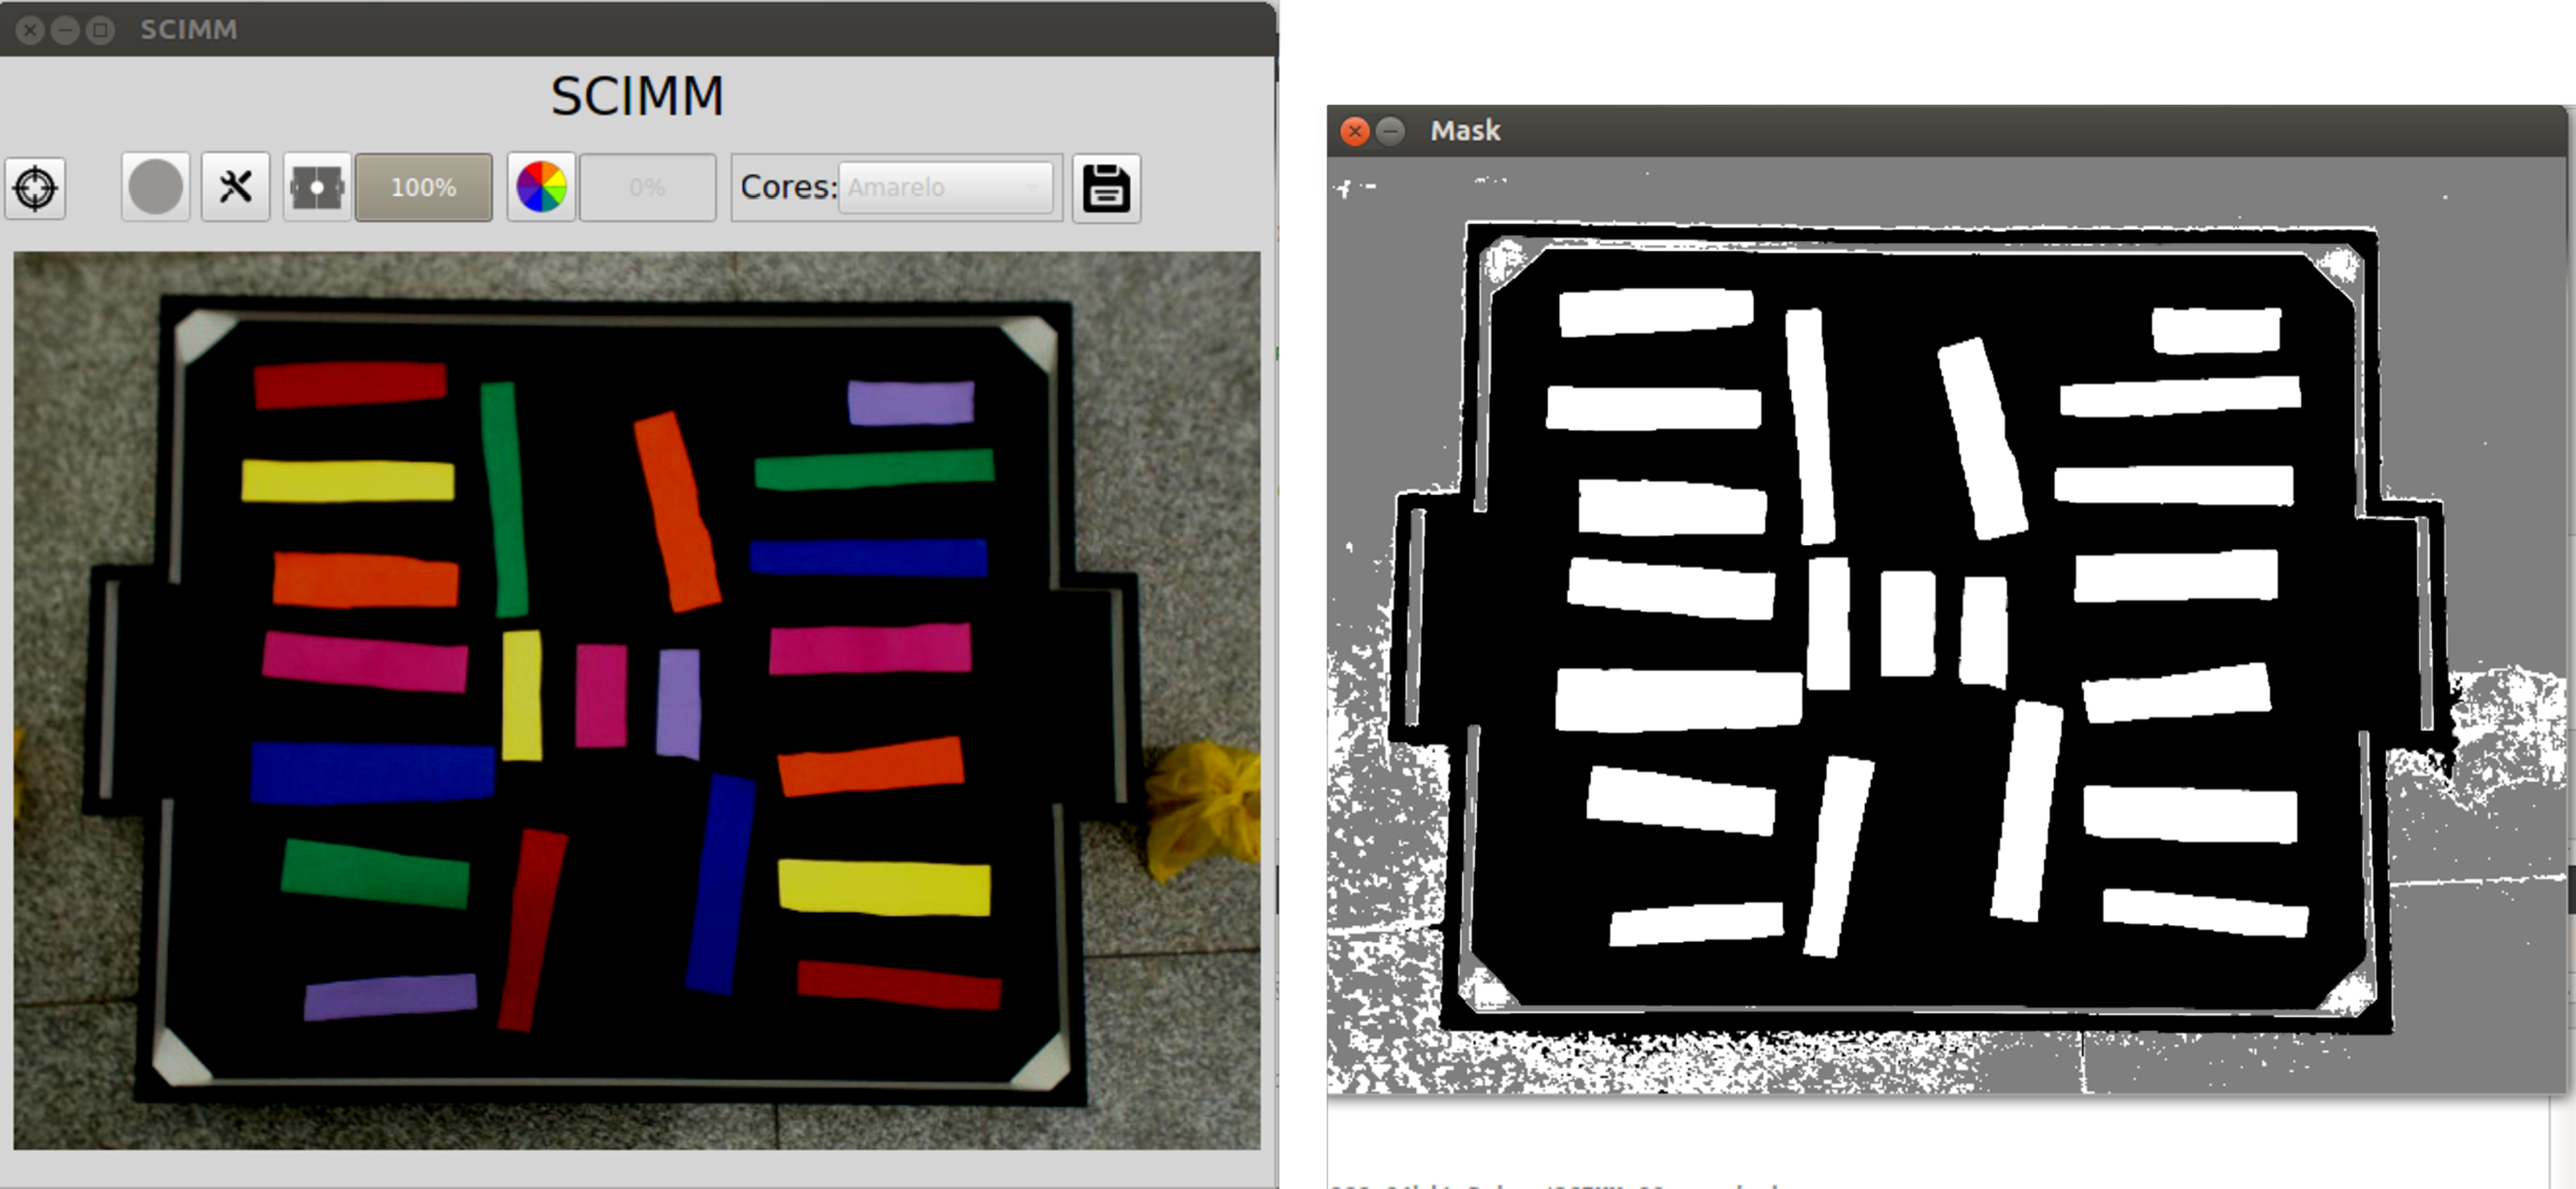
\includegraphics[width=0.98\textwidth]{passo3.pdf}
	\caption{Gráfico após escolhas de mínimos e máximos.}
	\label{GraficoGerado2}
\end{figure}
Usando os Sliders ou Entrada de Texto(explicados na sessão 4.1) são selecionados os valores mínimos e máximos para H, S e V. Durante a seleção dos valores o gráfico é atualizado para melhor visualização das ocorrências.
\section{Arquivo Final}

Arquivo gerado apos valores serem selecionados e salvos. Para cada cor selecionado são feitas duas linhas, a primeira contendo os valores mínimos e a segunda os valores máximos, no inicio de cada linha há o índice da cor.
  \begin{figure}[!h]
  	\centering
  	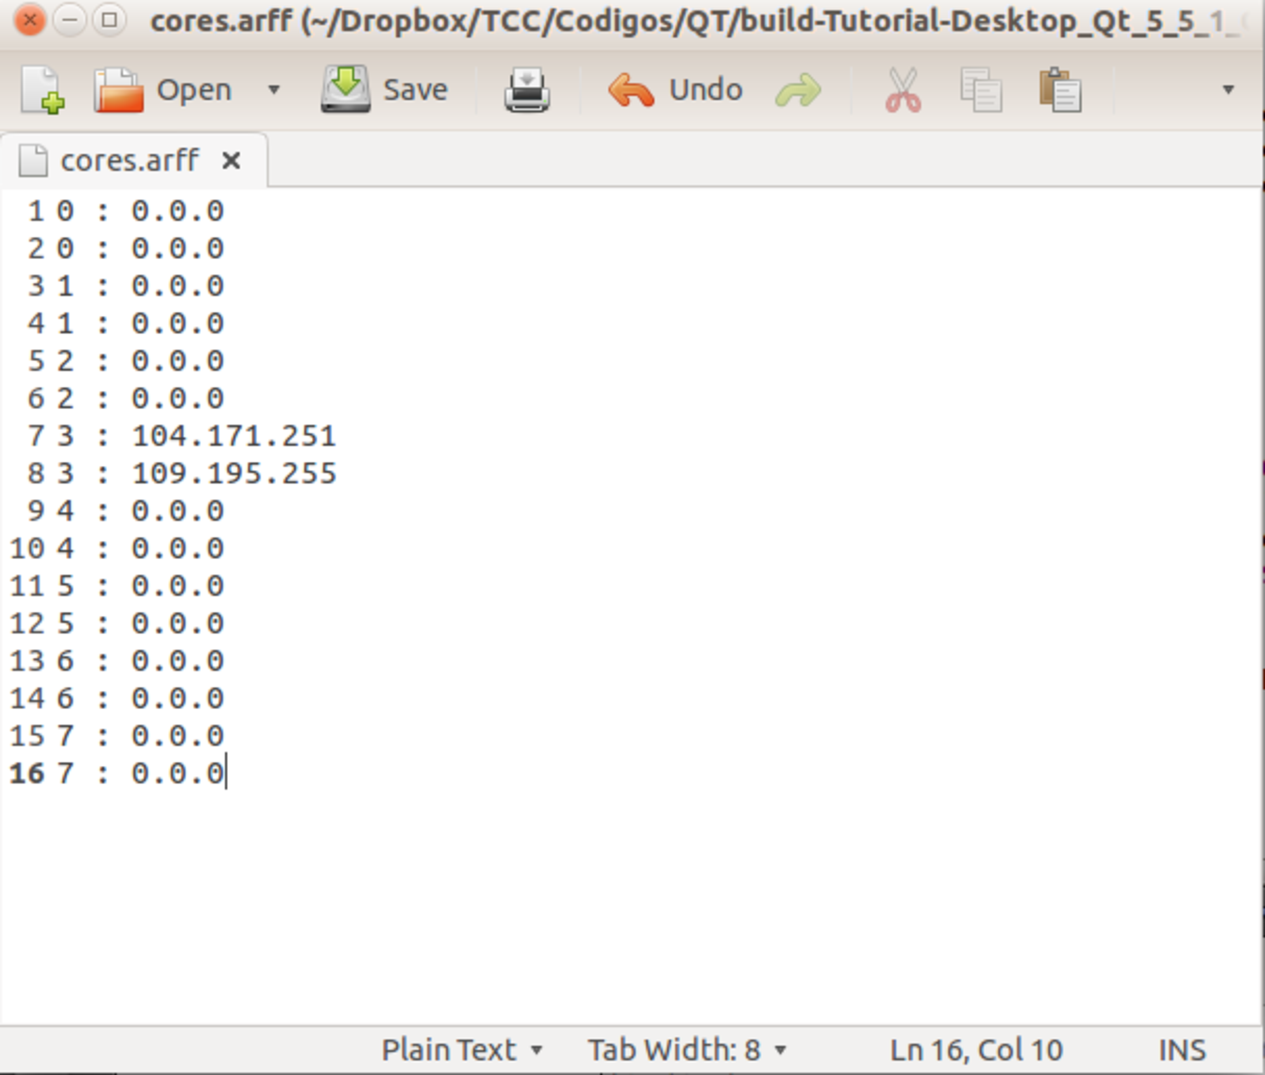
\includegraphics[width=0.7\textwidth]{arquivoResultado.pdf}
  	\caption{Arquivo com minimo e máximo dos valores HSV para cada cor.}
  	\label{ArquivoValores}
  \end{figure}
  \newpage
	
\newpage
 % Aplicação
%====================================================================================================
% ?????
%====================================================================================================
% TCC
%----------------------------------------------------------------------------------------------------
% Autor				: Jasane Schio
% Orientador		: Gedson Faria
% Co-Orientador		: Angelo Darcy
% Instituição 		: UFMS - Universidade Federal do Mato Grosso do Sul
% Departamento		: CPCX - Sistema de Informação
%----------------------------------------------------------------------------------------------------
% Data de criação	: 01 de Outubro de 2015
%====================================================================================================
% 
\chapter{Testes e Resultados} 
Este capitulo será dividio em duas seções: \textbf{Calibração} e \textbf{Testes}. A seção \textbf{Calibração} tera a descrição do processo de calibração de cores, a preparação do campo, configuração de imagem, etc. A seção \textbf{Testes} é onde descrevo o testes usados para a análise de eficiência do sistema desenvolvido.
\section{Calibração}
A calibração aqui descrita ocorreu dia no 19 de Agosto de 2016, entre 17:36 e 17:39.
A rotina de calibração do sistema, já descrita no Capitulo 3 deste trabalho, envolve primeiramente uma aquisição da imagem do campo vazio, sem nada no mesmo, como visto na Figura \ref{campovazio}.
\begin{figure}[H]
		\centering
		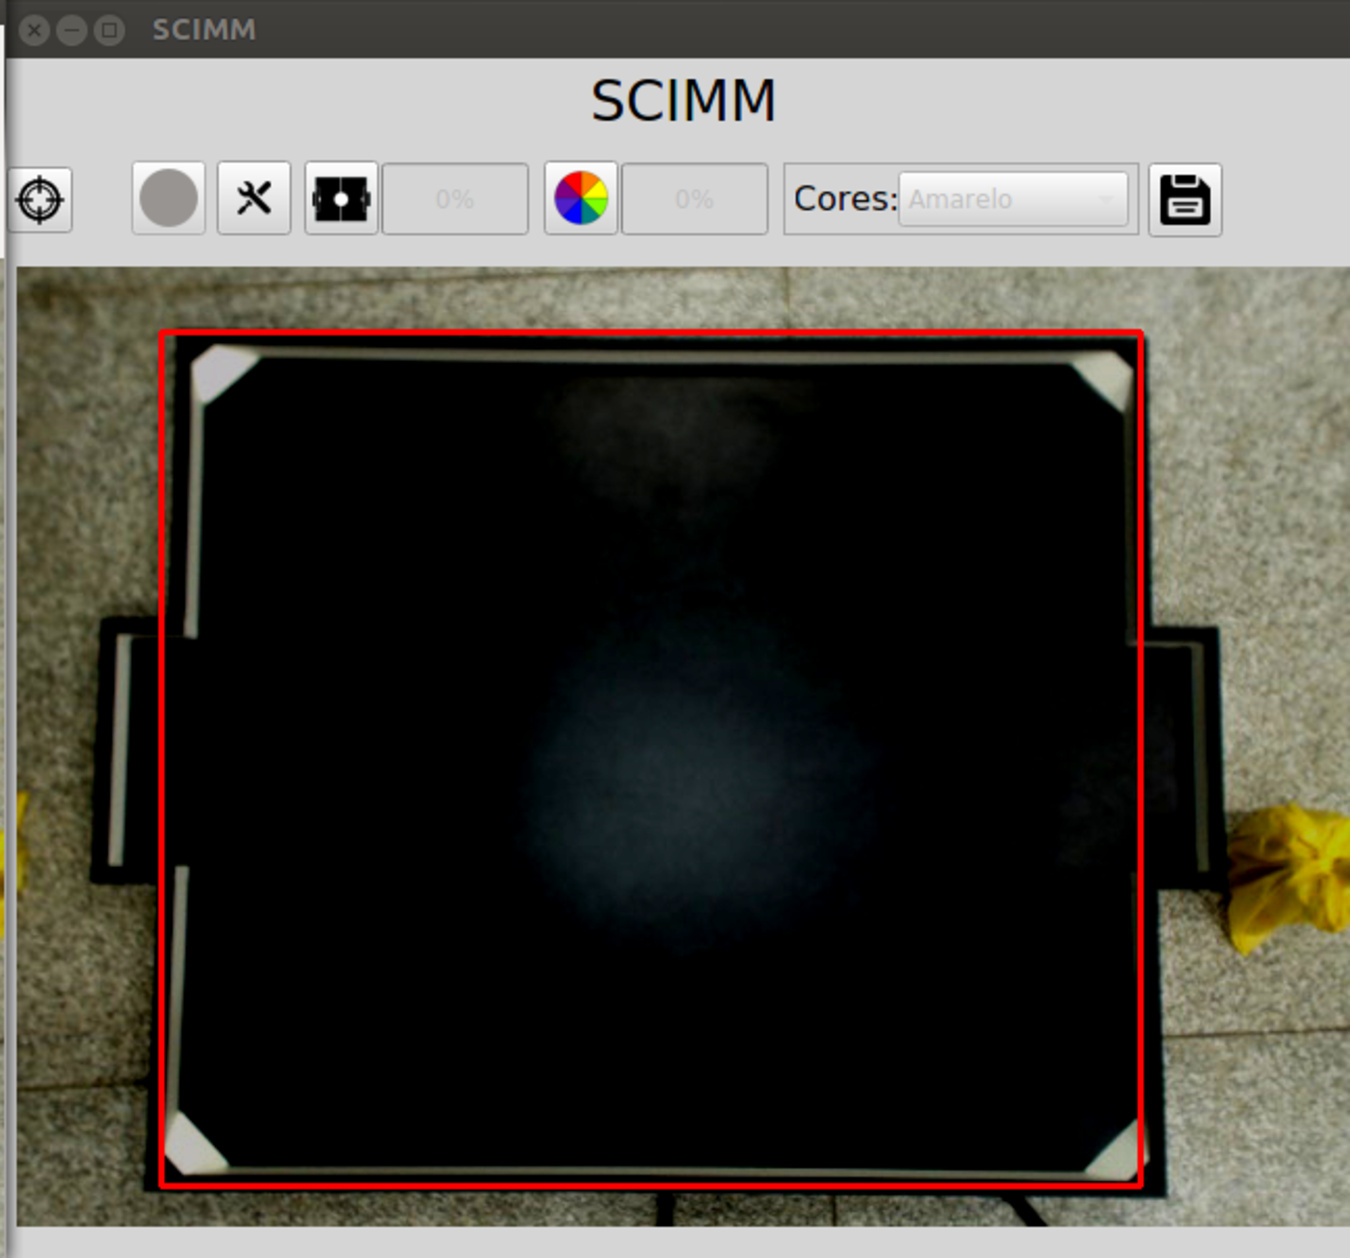
\includegraphics[width=0.45\textwidth]{fundoteste.pdf}
		\caption{Imagem do fundo com a seleção de campo}
		\label{campovazio}
	\end{figure}
Após ter o campo identificado pelo sistema, deve-se dispor sobre o campos os objetos coloridos, com as cores cujo se deseja obter o intervalo. É preferido que se usem tiras coloridas em vez de quadrado, de \textit{4cm x 4cm} como é comumente feito. Essa preferência se dá pois quanto maior o tamanho da tira de cor, maior sera o espectro de cores que seja analisado, assim sendo possível uma melhor qualidade de calibração.
Neste teste foram dispostos no campo tiras coloridas com largura entre \textit{17cm} e \textit{40cm} e altura entre \textit{5,5cm} e \textit{10,5cm}, cada cor com 3 tiras uma vez que o campo foi separado em três partes, significando as partes com diferentes luminosidades, sendo assim cada uma das tiras colocada em uma das partes do campos, como é possível visualiar na Figura \ref{fig:objetodispostos}.
	
	\begin{figure}[H]
%\begin{minipage}[H]{0.34\linewidth}
%\hspace{0.5cm}
\centering
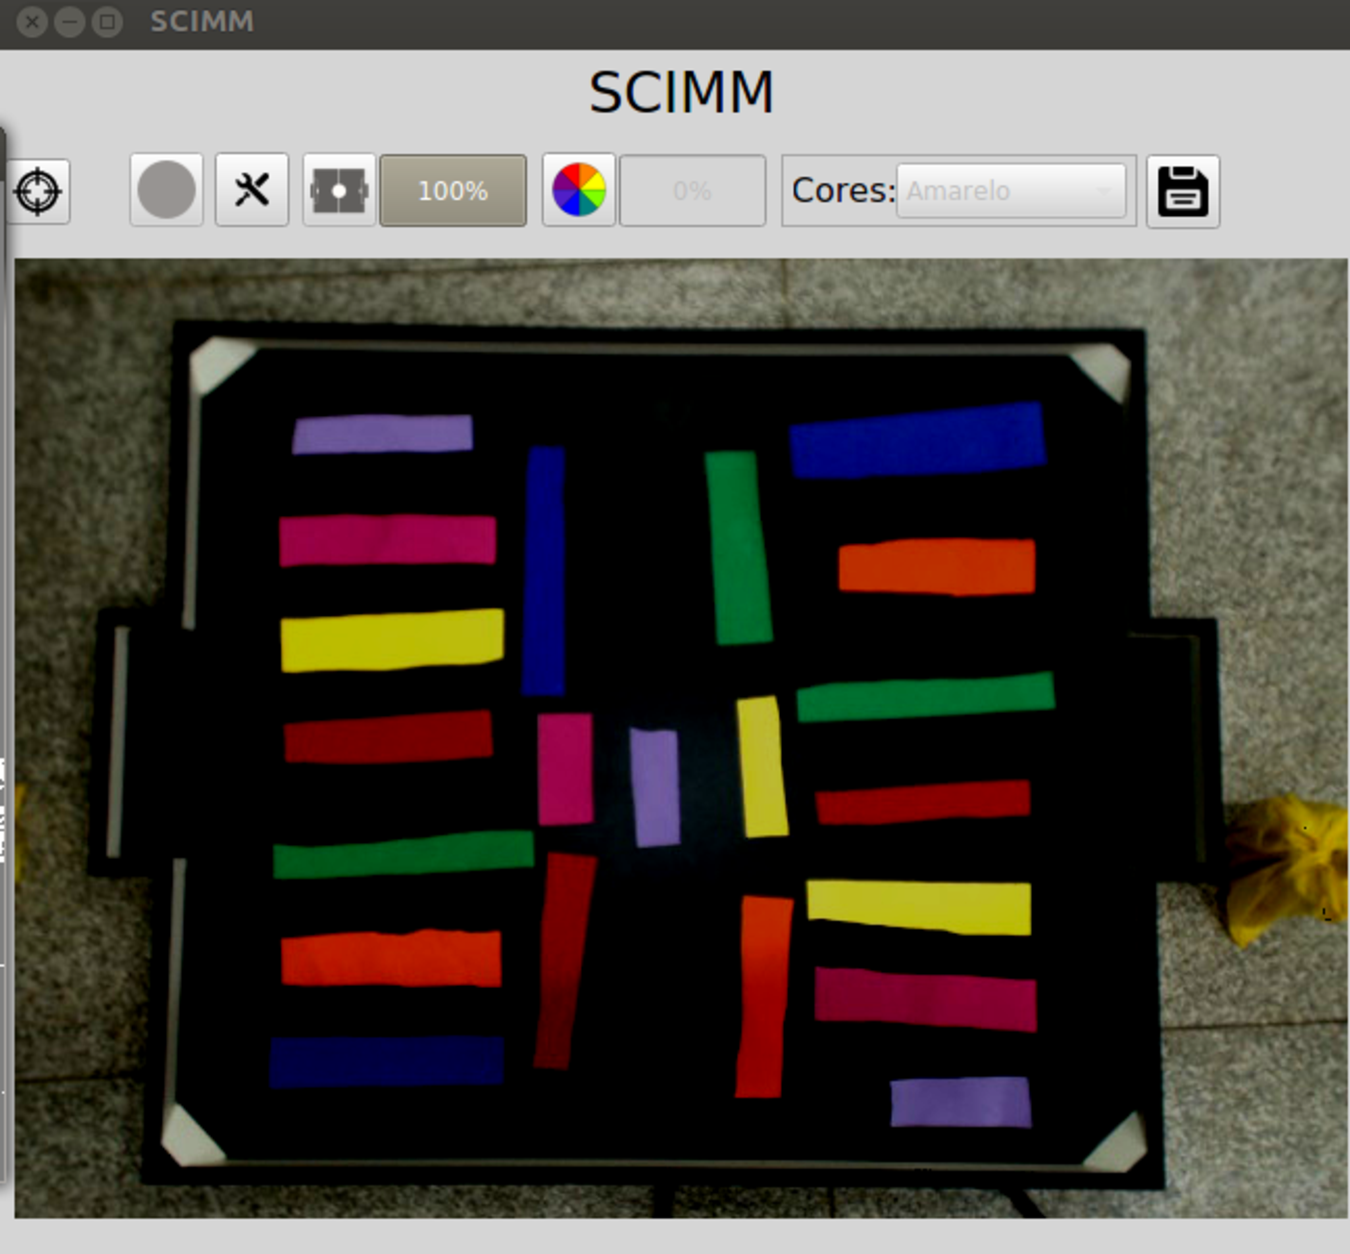
\includegraphics[width=0.45\textwidth]{objetosdispostos.pdf}
\caption{Objetos dispostos no campo para calibração}
\label{fig:objetodispostos}
%\end{minipage}
%\hspace{0.5cm}
%\begin{minipage}[H]{0.40\linewidth}
%\centering
%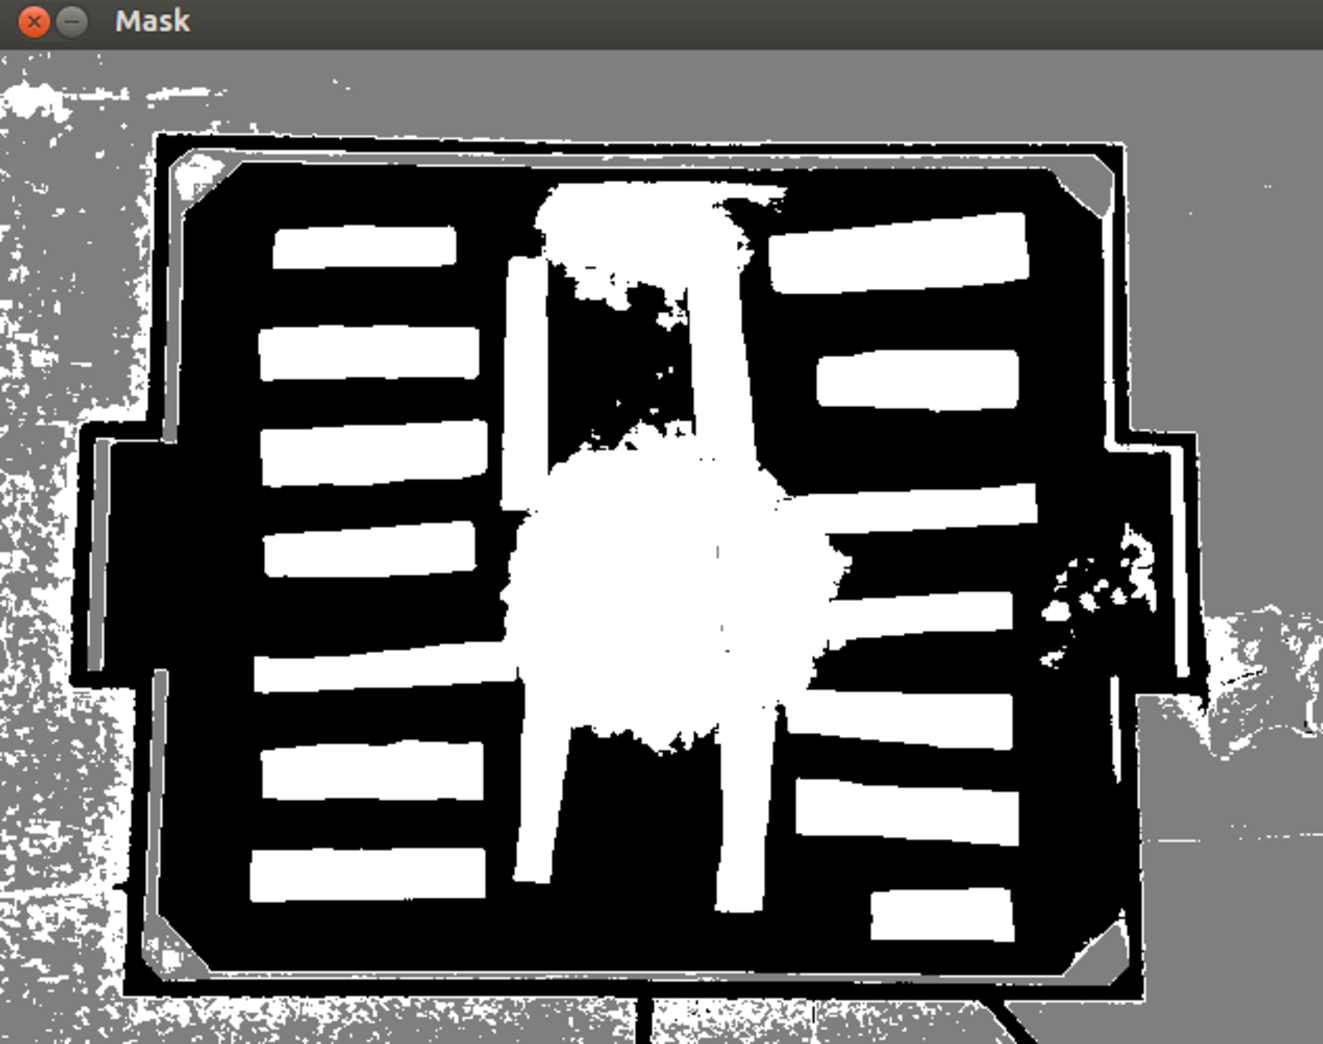
\includegraphics[width=\textwidth]{mascaragerada.pdf}
%\caption{Mascara gerada a partir da subtração de fundo}
%\label{fig:mascaragerada}
%\end{minipage}
\end{figure}	
	
Como resultado da rotina de calibraç\~{a}o foi gerado um arquivo .arff contendo 14 linhas. O arquivo é descrito na tabela abaixo:
	\begin{table}[H]
\centering 
\begin{tabular}{l|c|c|c}
Linha & Conteudo & Descrição  \\% Note a separação de col. e a quebra de linhas
\hline                               % para uma linha horizontal
 1& 21.50.50  &   Valor mínimo da cor Amarelo \\ \hline  
2& 30.255.255  &  Valor máximo da cor Amarelo \\  \hline 
3& 92.100.100  &   Valor mínimo da cor Azul \\  \hline 
4& 120.255.255  &  Valor máximo da cor  Azul \\  \hline 
5& 62.30.100 &  Valor mínimo da cor Verde \\  \hline 
6& 90.255.255  &  Valor máximo da cor Verde \\  \hline 
7& 169.100.100  &  Valor mínimo da cor Vermelho \\  \hline 
8& 179.255.255  &  Valor máximo da cor Vermelho \\   \hline 
9& 0.100.100  &  Valor mínimo da cor Laranja \\  \hline 
10& 20.255.255 &  Valor máximo da cor  Laranja \\  \hline 
11& 161.100.100 &  Valor mínimo da cor Rosa \\  \hline 
12& 168.255.255 &   Valor máximo da cor Rosa \\  \hline 
13& 126.30.30 &  Valor mínimo da cor Roxo \\  \hline 
14& 160.255.255 &  Valor máximo da cor Roxo \\  \hline 

\end{tabular}
\caption{Arquivo cores.arff}
\end{table}





 \section{Testes}
O teste aqui descrito ocorreu dia no 26 de Agosto de 2016, entre à 13:28 e 16:28.
Para elaboração do teste optou-se por dividir o campos no maior numero de partes possiveis, e ainda assim que essas partes coubessem todas as 7 cores usadas. Essa divisão foi feita para simular as cores em todas as partes possiveis do campos. O campo foi divido então em 15 partes de \textit{29cm} por \textit{41cm}, nomeadas alfabeticamente de A à O, como mostrado na Figura \ref{campodivisao}.

\begin{figure}[H]
		\centering
		\includegraphics[width=0.3\textwidth]{campodivisao.pdf}
		\caption{Divisão do campo em quinze partes nomeadas alfabeticamente.}
		\label{campodivisao}
	\end{figure}
	
Em cada uma das partes do campo estavam dispostas sete cores. Vermelho, Amarelo e Azul na primeira linha. Verde, Roxo, Laranja e Rosa na segunda. As cores estão distantes verticalmente \textit{6cm}, na primeria linha a distância entre as cores é de \textit{7,25cm} e na segunda linha de \textit{5cm}. Um  melhor detalhamento da disposição das cores é mostrado na Figura \ref{disposicaoparte}.


\begin{figure}[H]
\begin{minipage}[b]{0.45\linewidth}
\centering
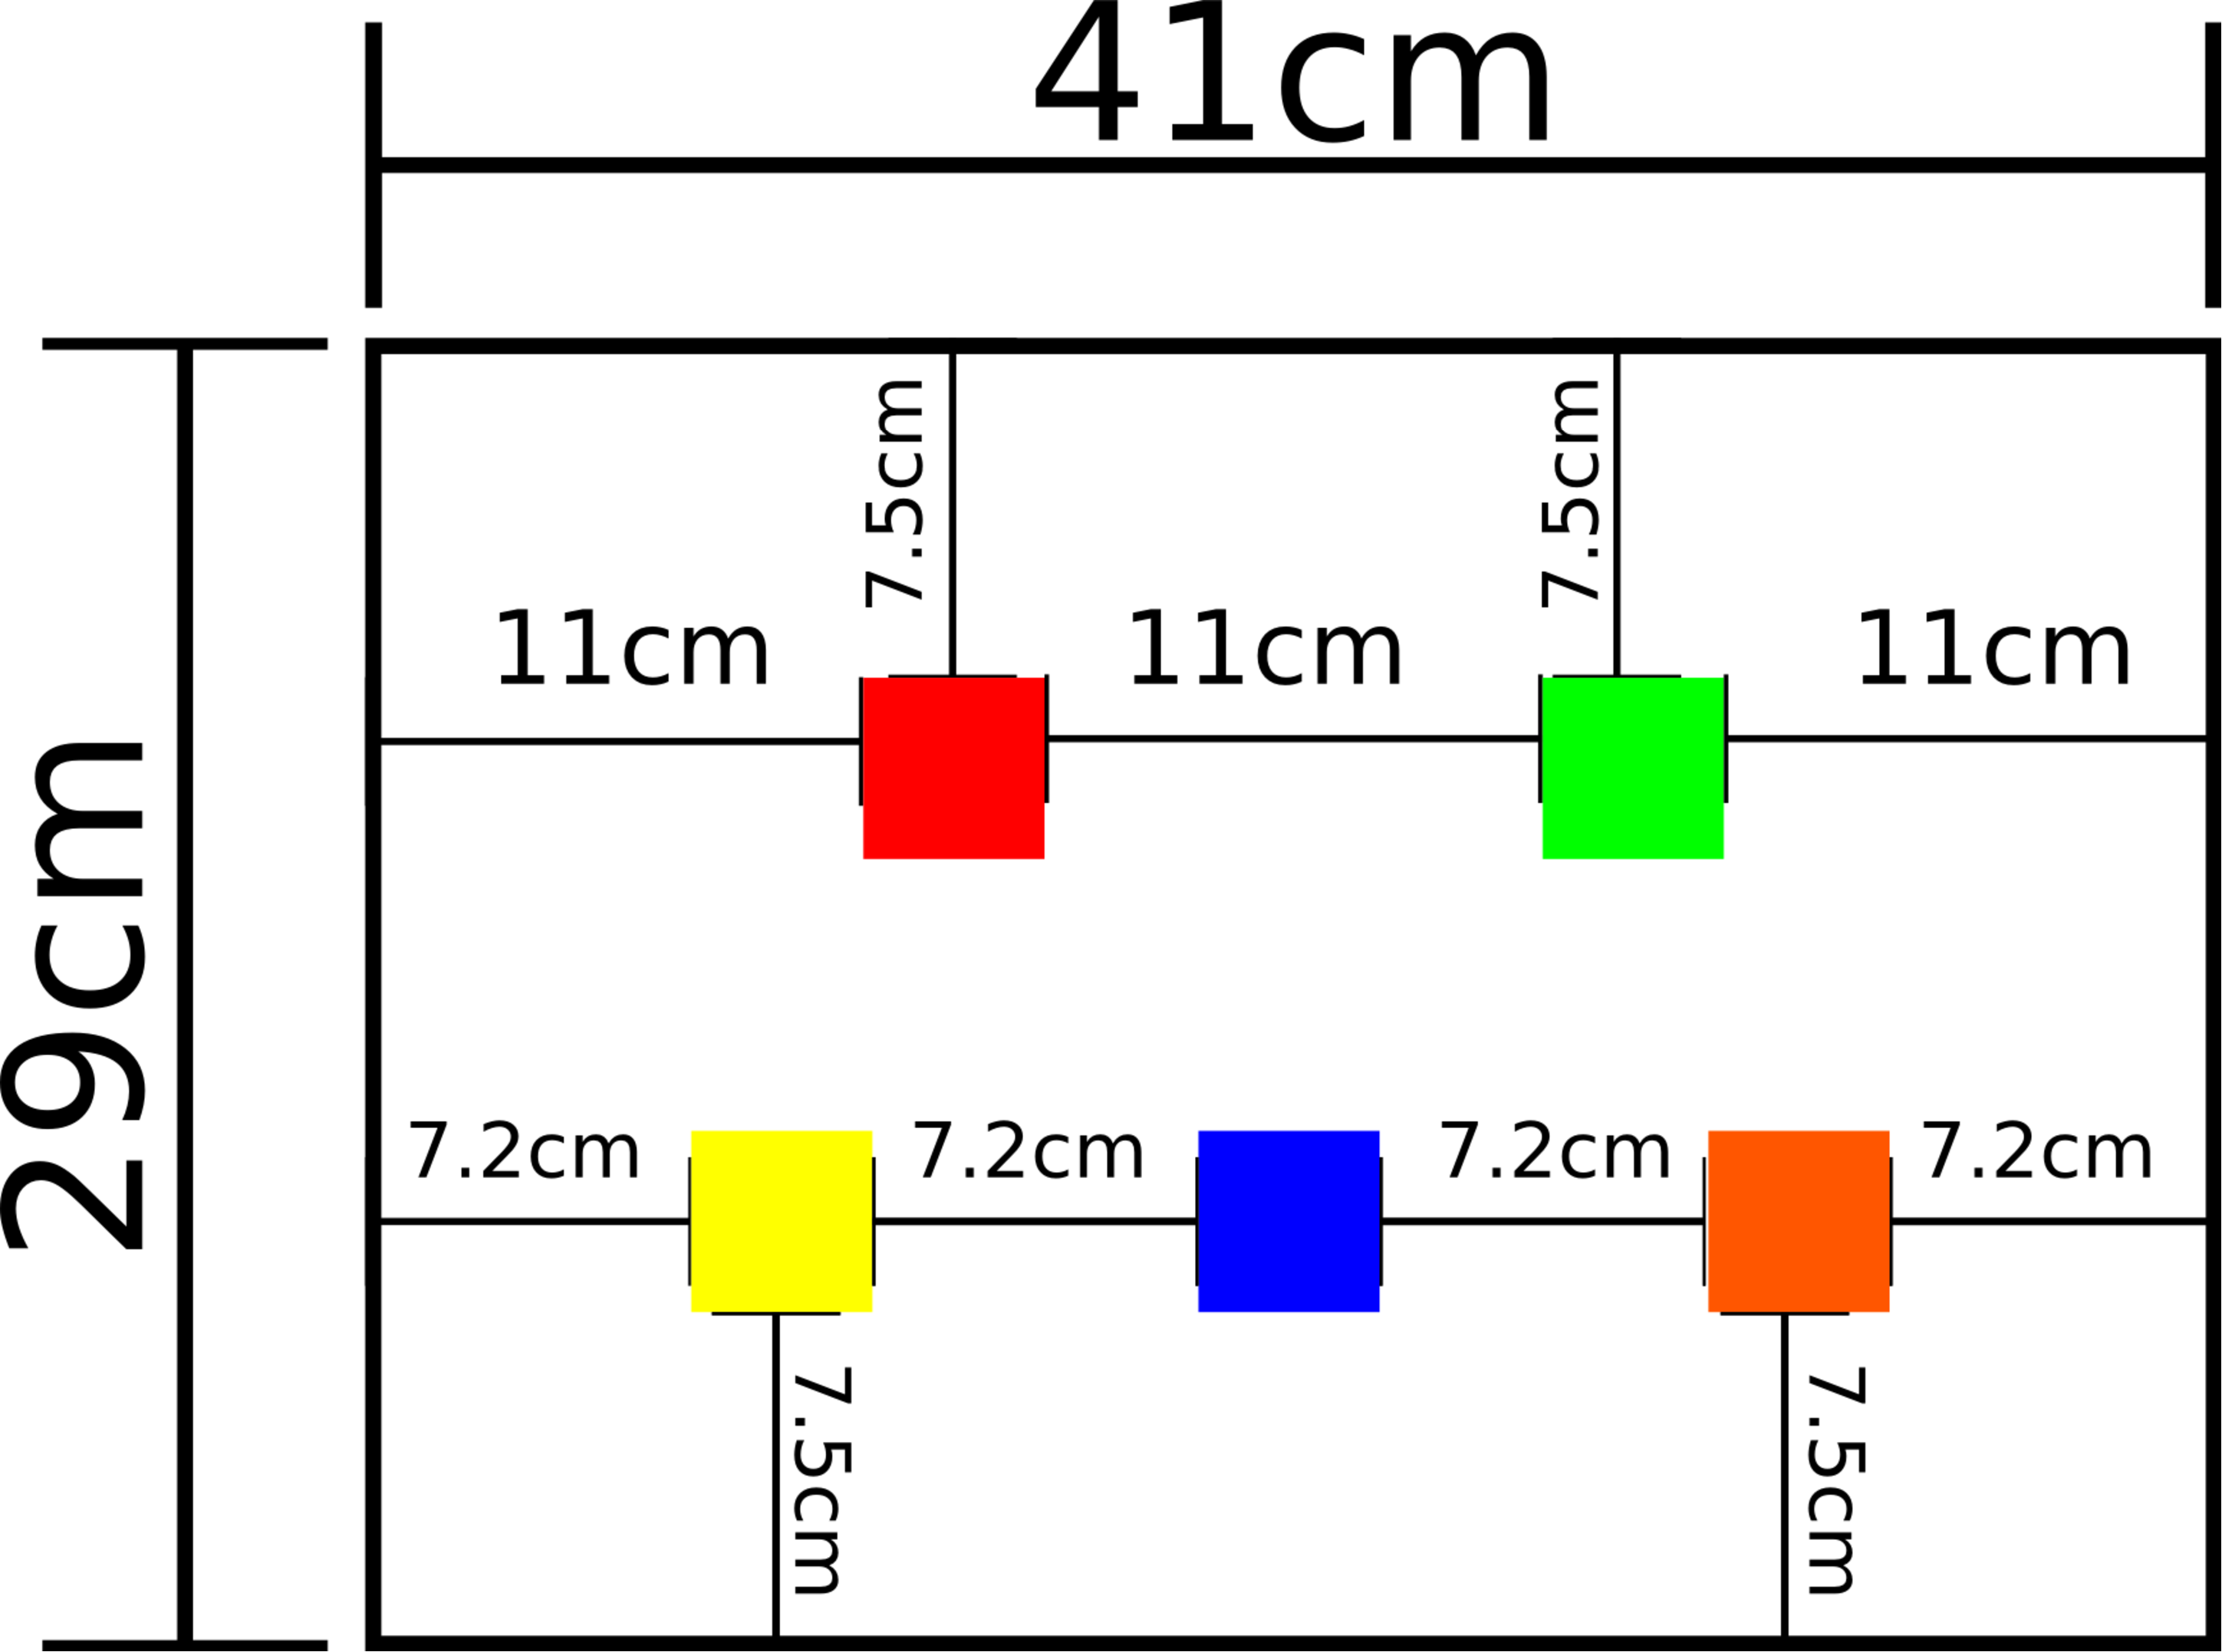
\includegraphics[width=\textwidth]{disposicaoparte.pdf}
\caption{Disposição de cada parte quanto as cores}
\label{fig:figure1}
\end{minipage}
\hspace{0.5cm}
\begin{minipage}[b]{0.45\linewidth}
\centering
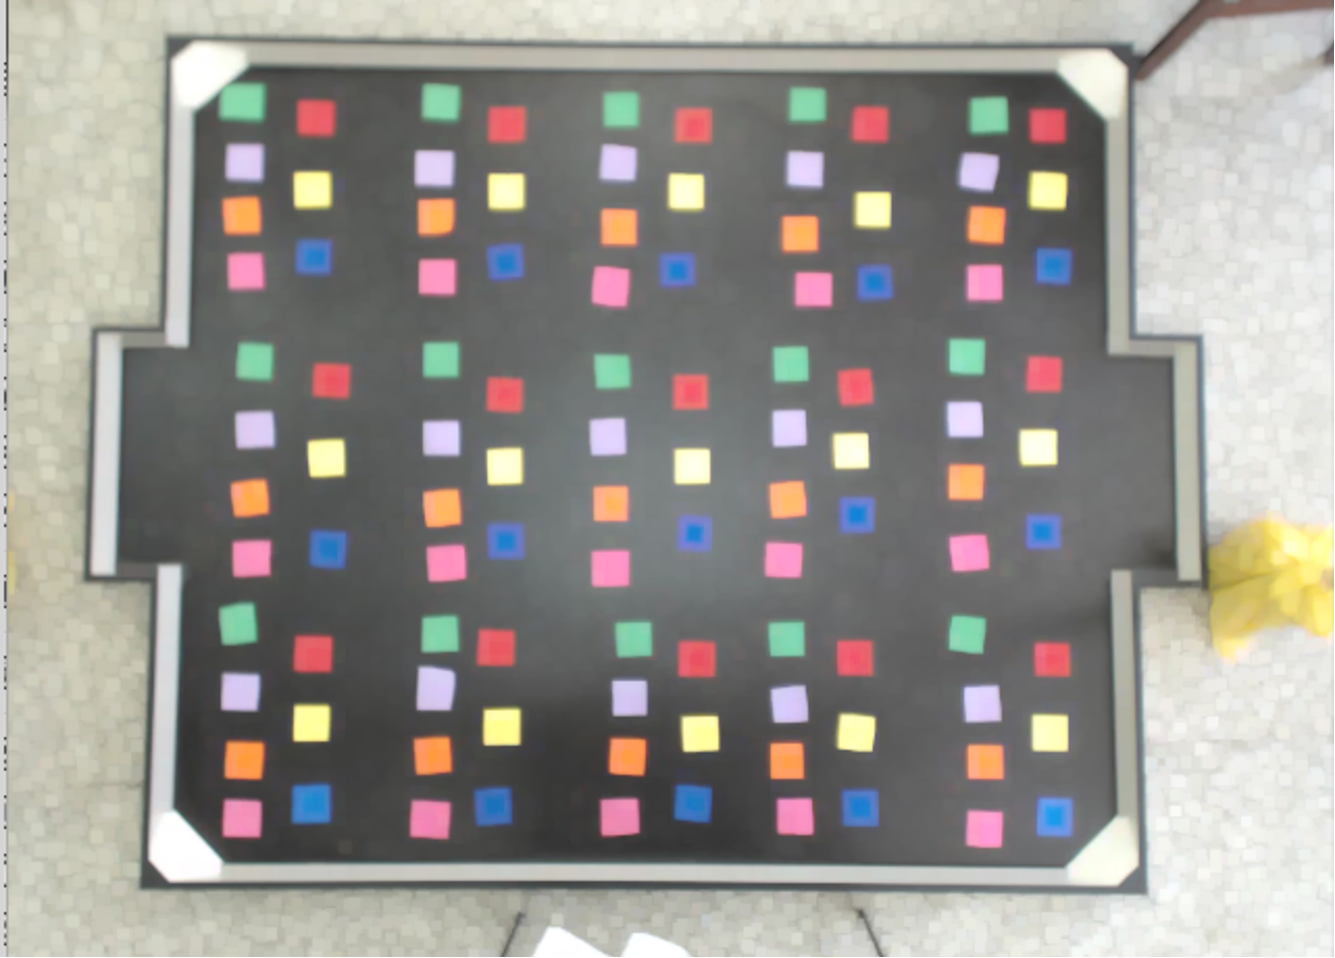
\includegraphics[width=\textwidth]{/testes/campofundo.pdf}
\caption{Campo após terem sido dispostas as cores}
\label{fig:figure2}
\end{minipage}
\end{figure}

\subsection{Cores Comuns}
\subsubsection{Amarelo}
	\begin{figure}[H]
		\centering
		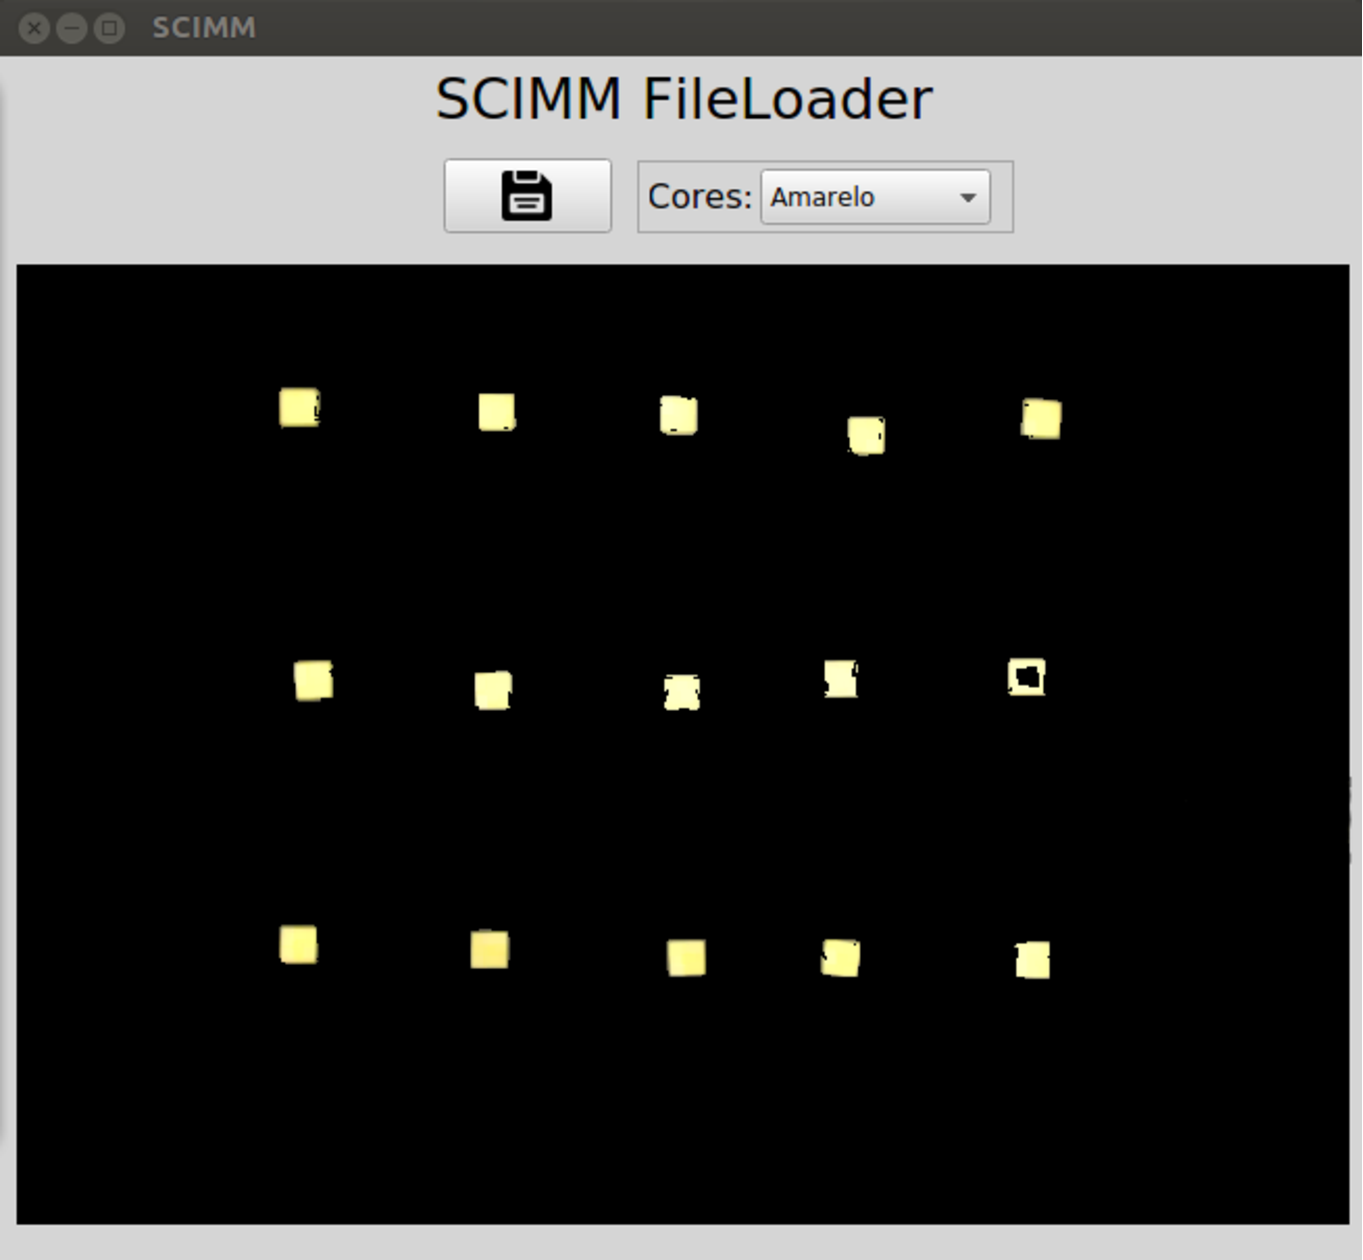
\includegraphics[width=0.5\textwidth]{/testes/amarelo.pdf}
		\caption{Imagem somente com os objetos dentro do intervalo do valor da cor amarela}
		\label{disposicaoparte}
	\end{figure}
	
	Dentre os objetos da cor amarela o sistema encontrou quatorze deles completamente e apenas um, que devido a luminosidade implicada em seu centro deixando a tonalidade muito perto do branco, não totalmente preenchido.
	
	\begin{table}[H]
\centering
\begin{tabular}{l|c|c}
Tipo de Objeto & Quantidade & \%  \\% Note a separação de col. e a quebra de linhas
\hline                               % para uma linha horizontal
Objetos Completos & 14 & 93,33 \\
\hline 
Objetos Com Falha de Preenchimento & 1 & 6,66 \\
\hline 
Objetos Com Diminuição de Contorno & 0 &\\
\hline 
Objetos Extrapolados & 0 &\\
\hline 
Objetos Com Diminuição de Área &  0 &\\
\hline 
Objetos Com Falhas Críticas & 0 &\\
\hline 
\end{tabular}
\caption{Categorização Dos Objetos}
\end{table}

Dentre as classficações dos objetos as que  \textit{Objetos Com Falhas Críticas} e \textit{Objetos Com Falha de Preenchimento} que juntos somam 6,66\% dos objetos.

\subsubsection{Azul}
	\begin{figure}[H]
		\centering
		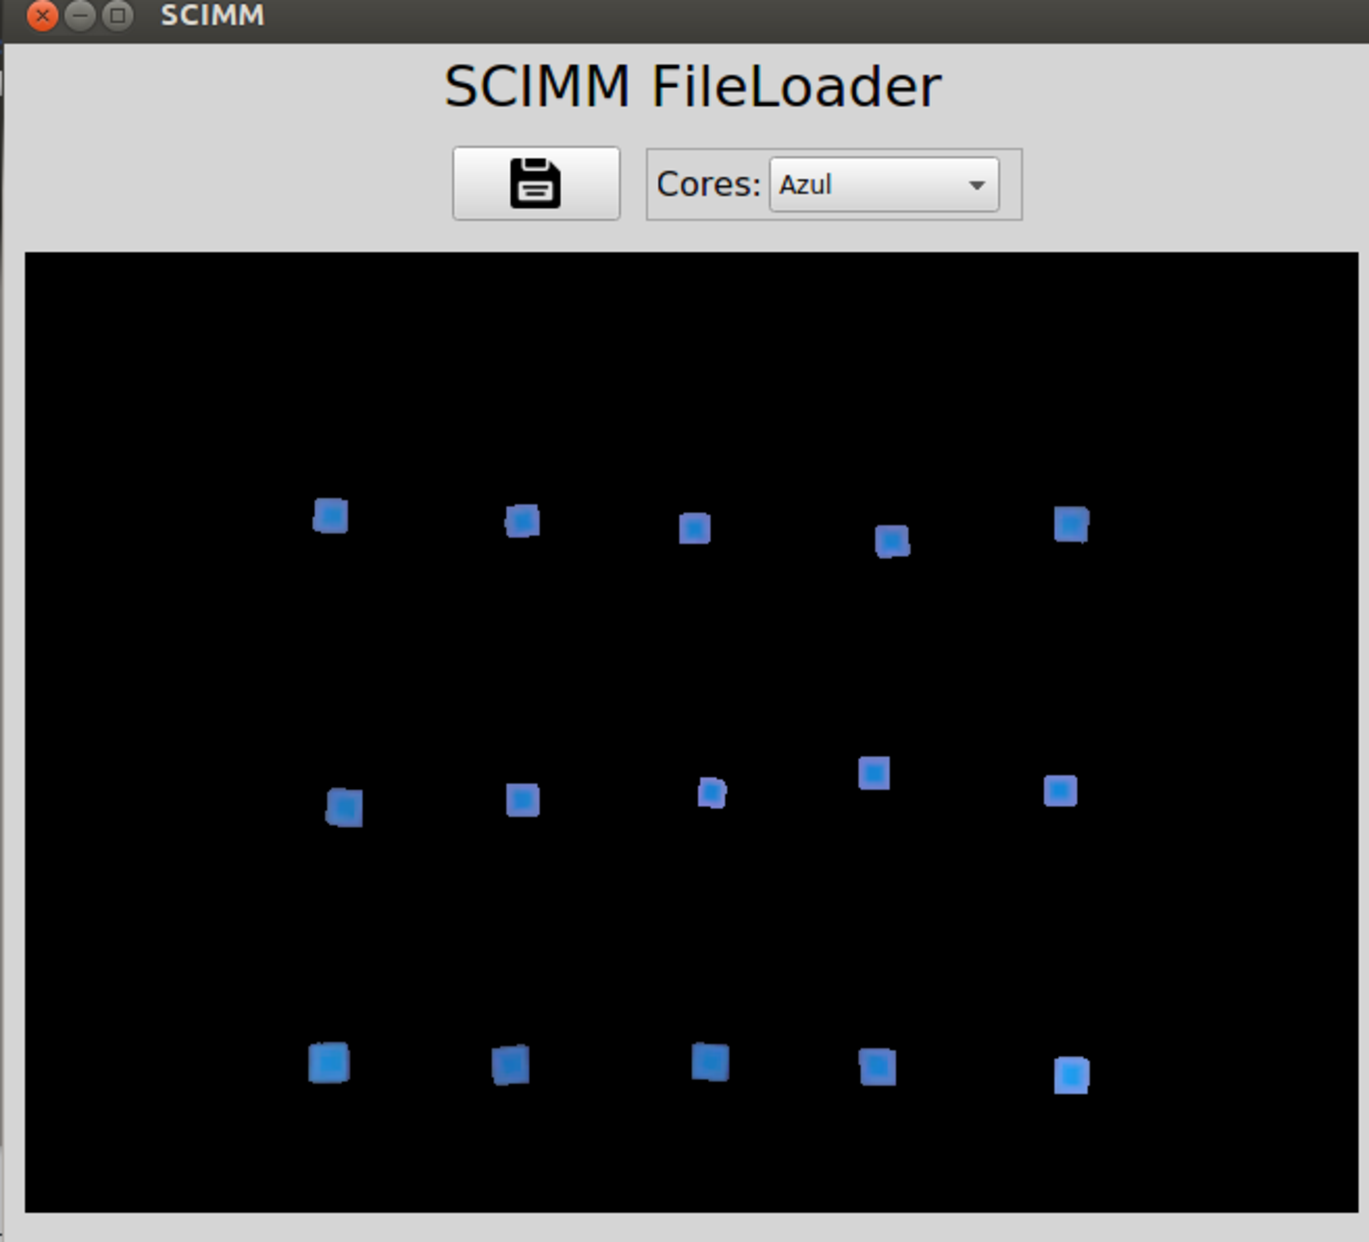
\includegraphics[width=0.5\textwidth]{/testes/azul.pdf}
		\caption{Imagem somente com os objetos dentro do intervalo do valor da cor azul}
		\label{disposicaoparte}
	\end{figure}

Os objetos da cor azul foram os que obtiveram os melhores resultados, os quinze objetos foram encontrados de forma preenchida.	Apesar dos quinze estarem totalmente preenchidos um dos objetos apresentou um tamanho reduzido aos demais devido ao fato de sua borda que não ter sido totamente detectada.

\begin{table}[h]
\centering
\begin{tabular}{l|c|c}
Tipo de Objeto & Quantidade & \% \\ % Note a separação de col. e a quebra de linhas
\hline                               % para uma linha horizontal
Objetos Completos & 14 & 93,33 \\
\hline 
Objetos Com Falha de Preenchimento & 0\\
\hline 
Objetos Com Diminuição de Contorno &  1 & 6,66
\\
\hline 
Objetos Extrapolados &  0\\
\hline 
Objetos Com Diminuição de Área & 0 \\
\hline 
Objetos Com Falhas Críticas & 0 \\
\hline 
\end{tabular}
\caption{Categorização Dos Objetos}
\end{table}

\subsubsection{Verde}
\begin{figure}[H]
		\centering
		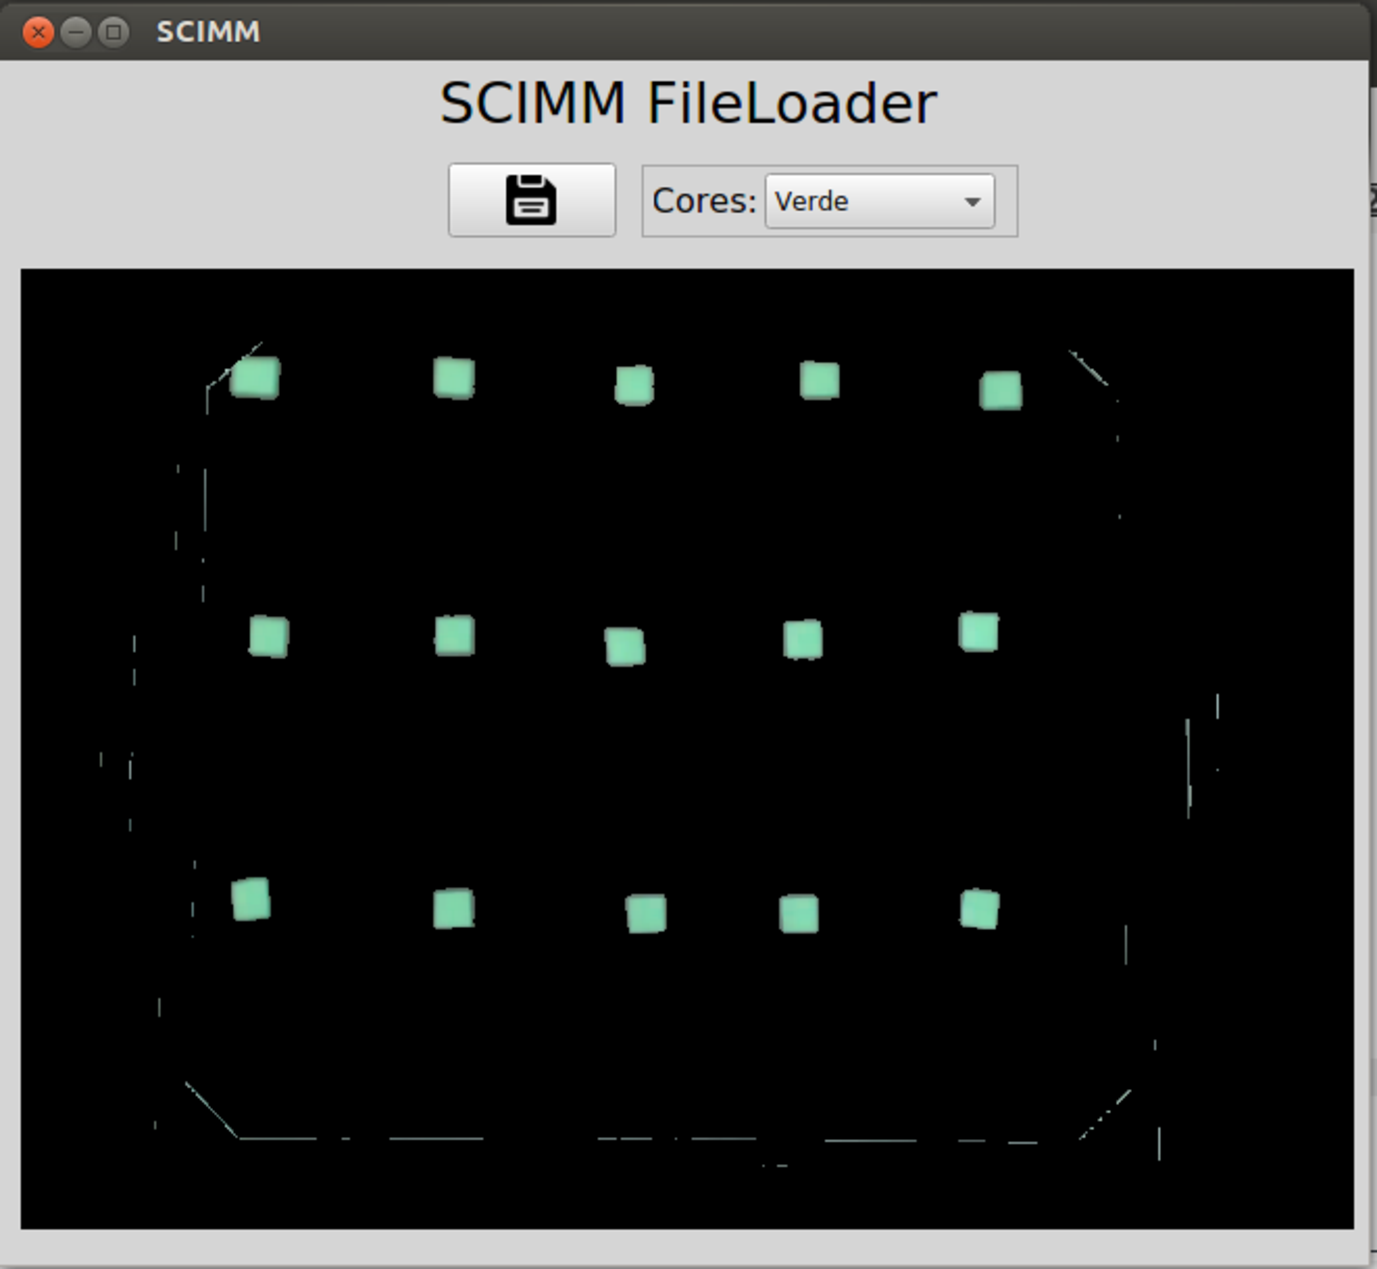
\includegraphics[width=0.5\textwidth]{/testes/verde.pdf}
		\caption{Imagem somente com os objetos dentro do intervalo do valor da cor verde}
		\label{disposicaoparte}
	\end{figure}

Os objetos da cor verde foram satisfatoriamente encontrados, com seu preenchimento total e não havendo perda de área devido a qualquer interferência de luz em sua borda.	
	
\begin{table}[h]
\centering
\begin{tabular}{l|c|c}
Tipo de Objeto & Quantidade & \% \\ % Note a separação de col. e a quebra de linhas
\hline                               % para uma linha horizontal
Objetos Completos &  15 &100 \\
\hline 
Objetos Com Falha de Preenchimento & 0\\
\hline 
Objetos Com Diminuição de Contorno &  0\\
\hline 
Objetos Extrapolados & 0 \\
\hline 
Objetos Com Diminuição de Área &  0 \\
\hline 
Objetos Com Falhas Críticas & 0 \\
\hline 
\end{tabular}
\caption{Categorização Dos Objetos}
\end{table}	
\subsubsection{Rosa}
	
	\begin{figure}[H]
		\centering
		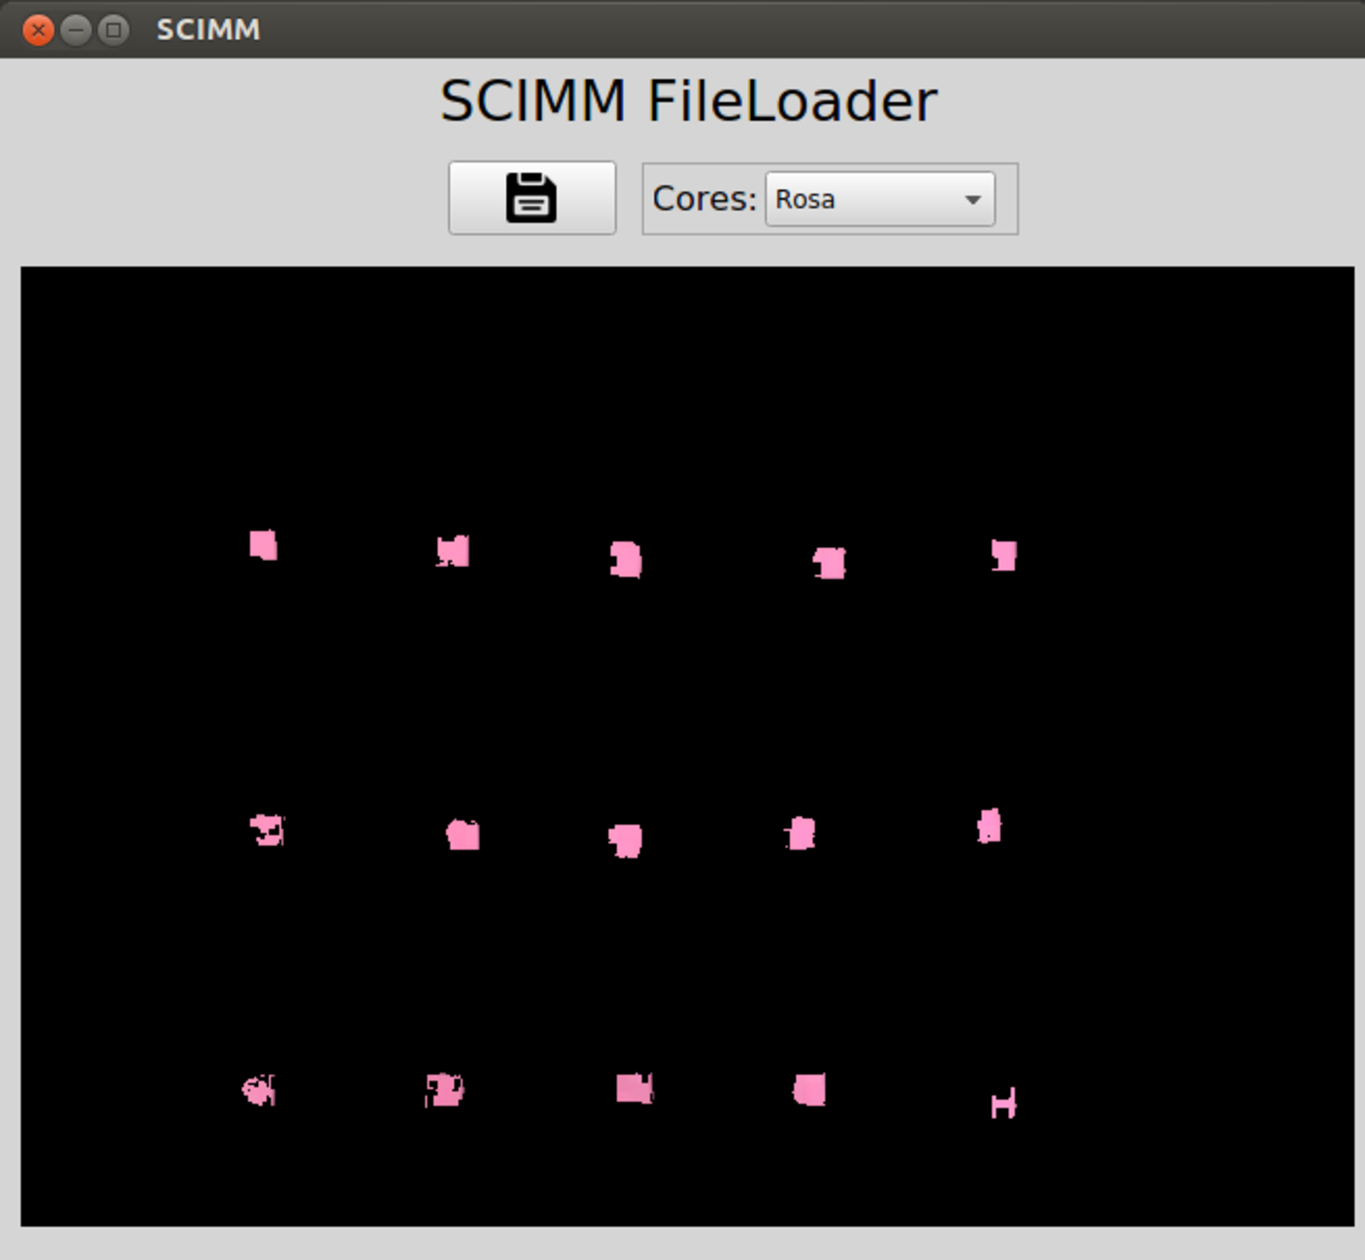
\includegraphics[width=0.5\textwidth]{/testes/rosa.pdf}
		\caption{Imagem somente com os objetos dentro do intervalo do valor da cor rosa}
		\label{disposicaoparte}
	\end{figure}
	
Dentre os objetos rosa detectados, quatro obtiveram falhas em sua detecção, falhas de preenchimento e diminuição de borda, estes podem ser desconsiderados dos objetos. Dentro os outros onze: três foram detectados sem falhas de preenchimentos apenas com diminuição de sua área para aproximadamente metade da área real do objeto; os outros oito foram encontrados apesas com diminuição de área devido a diminuição de borda.
	
	\begin{table}[h]
\centering
\begin{tabular}{l|c|c}
Tipo de Objeto & Quantidade  & \% \\ % Note a separação de col. e a quebra de linhas
\hline                               % para uma linha horizontal
Objetos Completos &  0\\
\hline 
Objetos Com Falha de Preenchimento & 0\\
\hline 
Objetos Com Diminuição de Contorno & 8& 53,33
 \\
\hline 
Objetos Extrapolados & 0 \\
\hline 
Objetos Com Diminuição de Área & 3 & 20\\
\hline 
Objetos Com Falhas Críticas & 4 & 26,66 \\
\hline 
\end{tabular}
\caption{Categorização Dos Objetos}
\end{table}

Dentre as classficações dos objetos as que  \textit{Objetos Com Falhas Críticas} e \textit{Objetos Com Falha de Preenchimento} que juntos somam 26,66\% dos objetos. Apesar de ser um numero não tão baixo, a cor rosa não é uma cor que a equipe Cedro costuma usar em seus jogos, sendo assim, essa taxa de erro não influencia na eficienca do sistema.
\subsubsection{Roxo}
\begin{figure}[H]
		\centering
		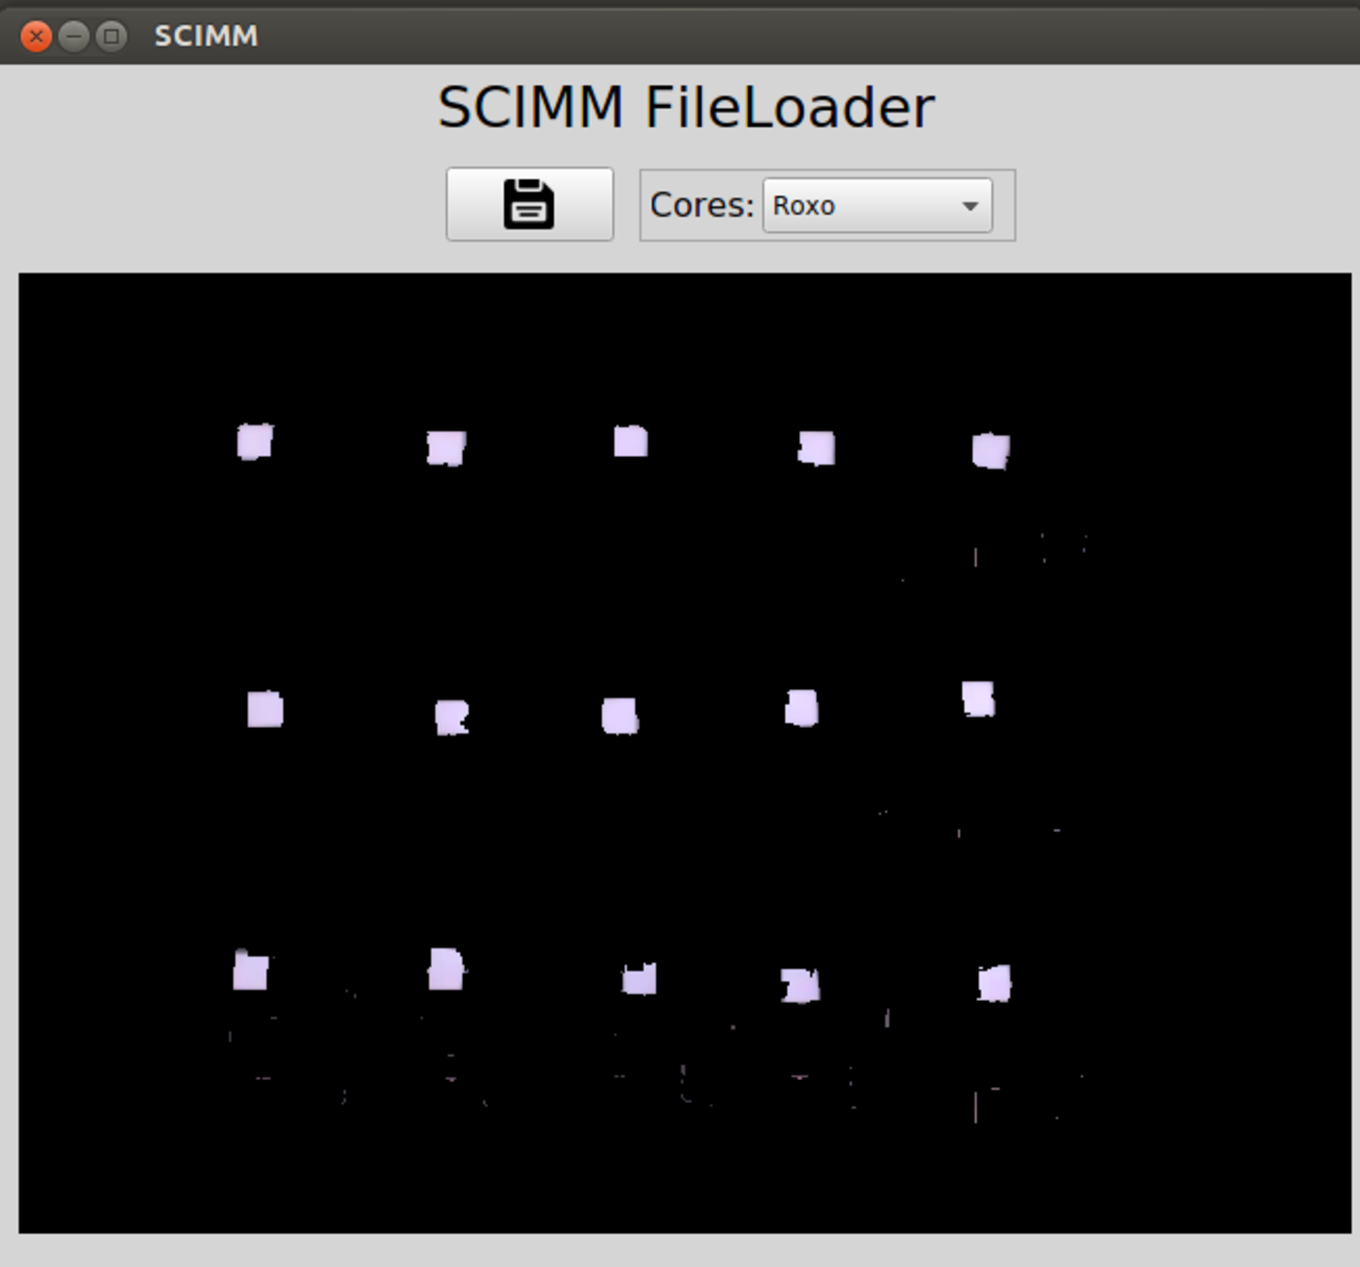
\includegraphics[width=0.5\textwidth]{/testes/roxo.pdf}
		\caption{Imagem somente com os objetos dentro do intervalo do valor da cor roxo}
		\label{disposicaoparte}
	\end{figure}

Todos os objetos roxos dispostos no campo foram encontrados pelo intervalo da cor. Dentre os quinze, quatro não apresentaram problema algum e foram completamente detectados; oito possuiram diminiução em seu contorno e três diminuição em sua área relativa.
\begin{table}[h]
\centering
\begin{tabular}{l|c|c}
Tipo de Objeto & Quantidade  & \% \\ % Note a separação de col. e a quebra de linhas
\hline                               % para uma linha horizontal
Objetos Completos &  4 & 26,66\\
\hline 
Objetos Com Falha de Preenchimento & 0 \\
\hline 
Objetos Com Diminuição de Contorno &  8 & 53,33\\
\hline 
Objetos Extrapolados & 0 \\
\hline 
Objetos Com Diminuição de Área & 3 & 20\\
\hline 
Objetos Com Falhas Críticas & 0 \\
\hline 
\end{tabular}
\caption{Categorização Dos Objetos}
\end{table}
	
\subsection{Cores Com Problemas Conhecidos}
Cores como Vermelho e Laranja possuem o problema de por vezes, devido a interferencia externas, se assemelharem a outras. Este problemas ja são de conhecimento da área.
	
	
\subsubsection{Vermelho}
	\begin{figure}[H]
		\centering
		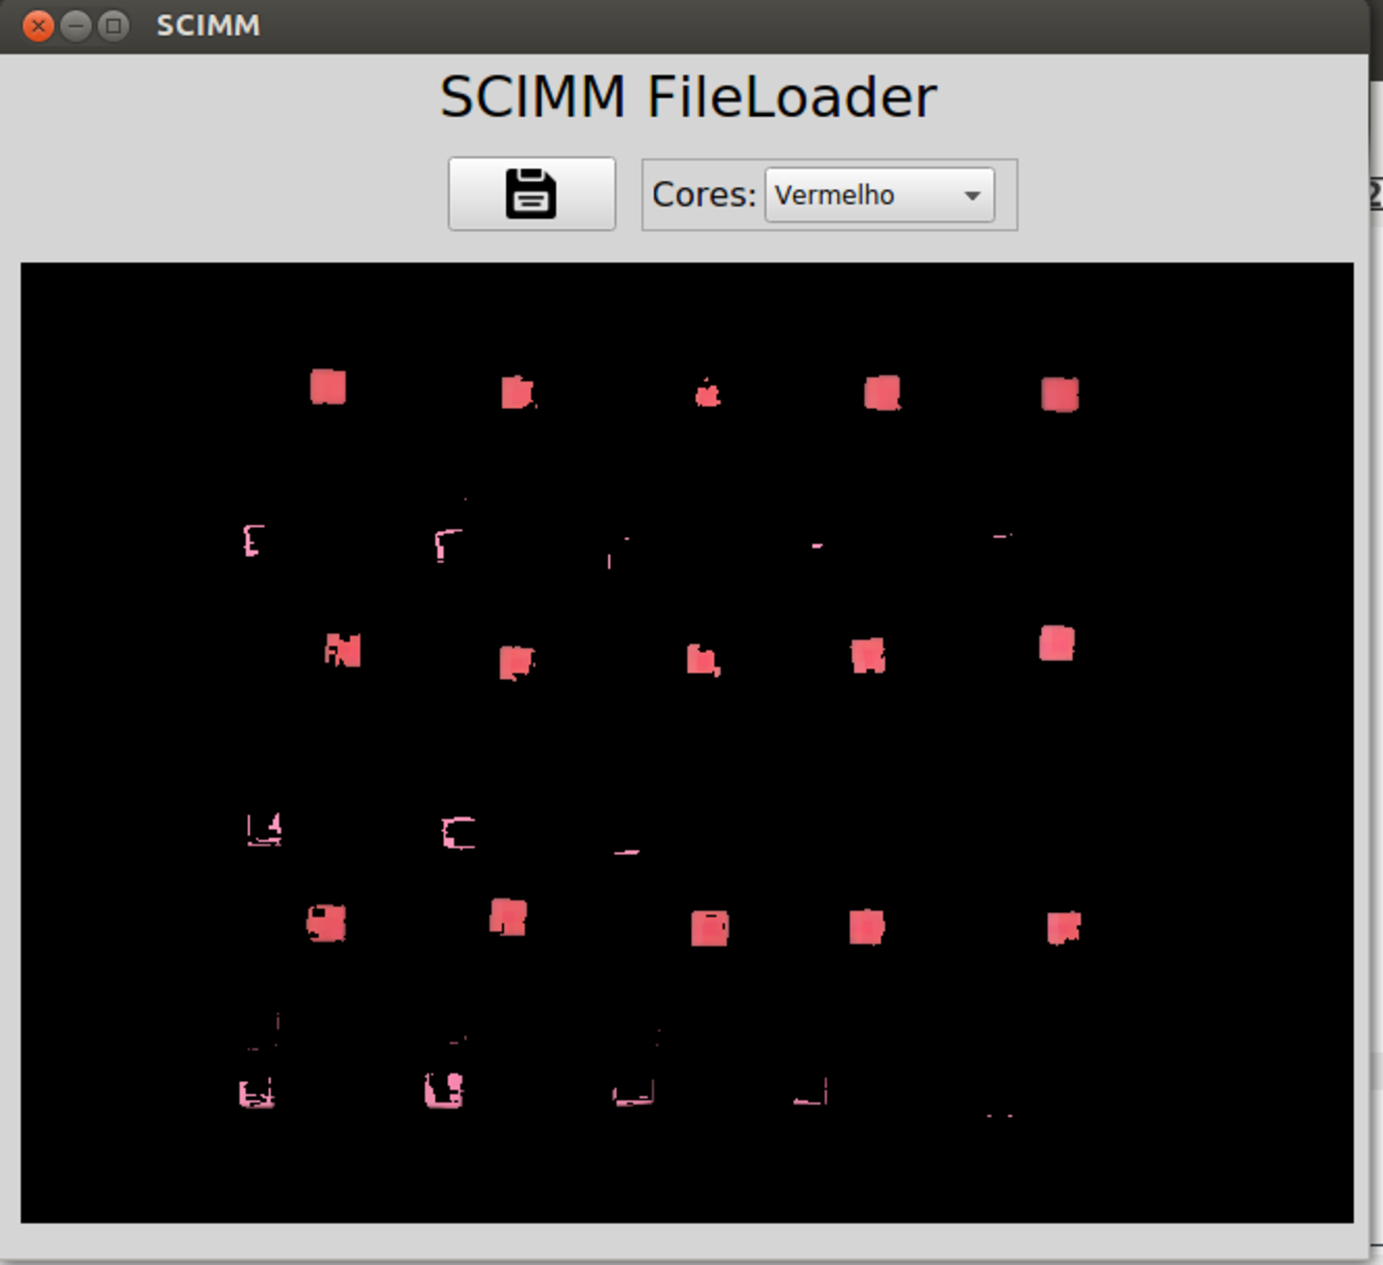
\includegraphics[width=0.5\textwidth]{/testes/vermelho.pdf}
		\caption{Imagem somente com os objetos dentro do intervalo do valor da cor vermelho}
		\label{disposicaoparte}
	\end{figure}

A cor rosa, em determinadas luminosidades pode acabar sendo semelhante a cor vermelha, por este motivo que alguns traços dos objetos rosas estão aparecendo dentro do intervalo de calibração. Porem serão ignorados, uma vez que é possível de ser feito a separação entre as das cores via software.	

	
	\begin{table}[h]
\centering
\begin{tabular}{l|c|c}
Tipo de Objeto & Quantidade  & \% \\ % Note a separação de col. e a quebra de linhas
\hline                               % para uma linha horizontal
Objetos Completos &  8 & 53,33 \\
\hline 
Objetos Com Falha de Preenchimento & 1 & 6,66 \\
\hline 
Objetos Com Diminuição de Contorno &  4 & 26,66 \\
\hline 
Objetos Extrapolados &  13 \\
\hline 
Objetos Com Diminuição de Área &  1 &6,66 \\
\hline 
Objetos Com Falhas Críticas &  1 & 6,66\\
\hline 
\end{tabular}
\caption{Categorização Dos Objetos}
\end{table}

Dentre as classficações dos objetos as que  \textit{Objetos Com Falhas Críticas} e \textit{Objetos Com Falha de Preenchimento} que juntos somam somente 13,32\% dos objetos.

\subsubsection{Laranja}
	\begin{figure}[H]
		\centering
		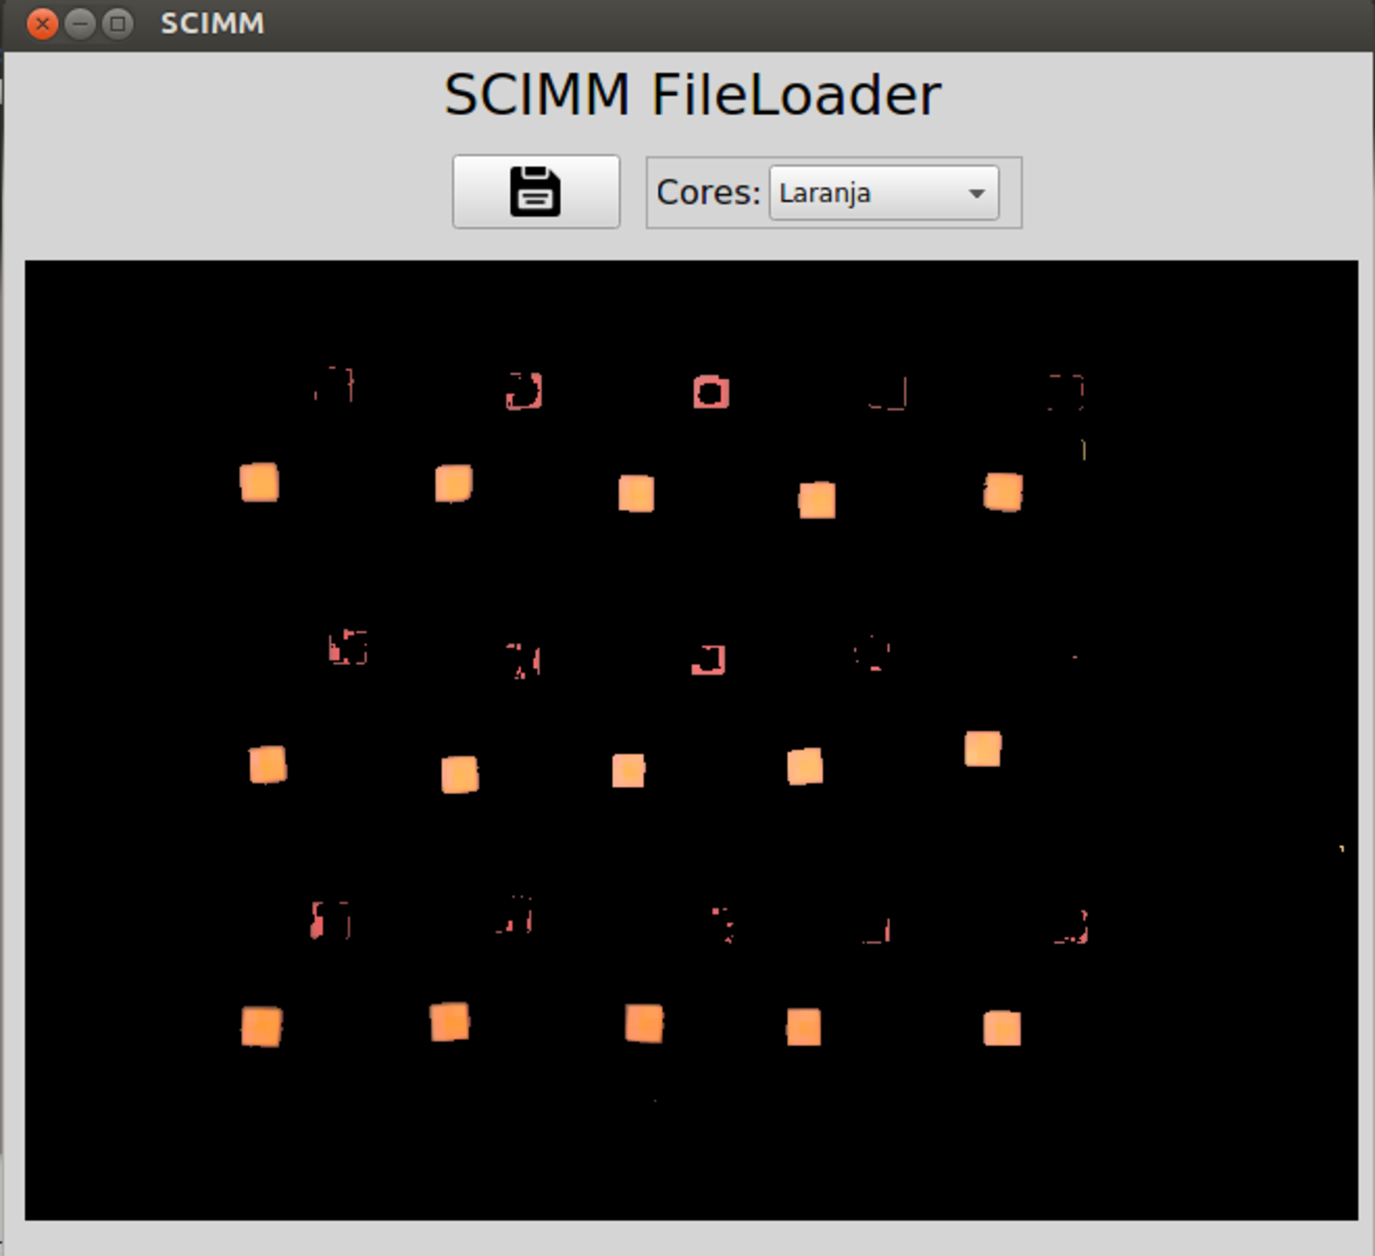
\includegraphics[width=0.5\textwidth]{/testes/laranja.pdf}
		\caption{Imagem somente com os objetos dentro do intervalo do valor da cor laranja}
		\label{disposicaoparte}
	\end{figure}
	
	Devido à um problema muito comum na área de calibração de cores, a cor laranja possui o problema de ser, por muitas vezes, semelhante a vermelha, e devido a luminosidade implicada tanto em uma quanto na outra, ambas as cores tendem a se tornarem próximas.
	Sabendo deste problema, o fato de terem sido encontrados objetos da cor vermelha dentro do intervalo de valores da cor laranja é ignorado e somente serão levados em consideração os objetos visualmente laranjas.
	Os quinze objetos da cor laranja foram encontrados com precisão. Todos possuindo seu completo preenchimento e borda.
	
\begin{table}[h]
\centering
\begin{tabular}{l|c|c}
Tipo de Objeto & Quantidade  & \% \\ % Note a separação de col. e a quebra de linhas
\hline                               % para uma linha horizontal
Objetos Completos &  15 & 100 \\
\hline 
Objetos Com Falha de Preenchimento & 0 \\
\hline 
Objetos Com Diminuição de Contorno &  0 \\
\hline 
Objetos Extrapolados & 8 \\
\hline 
Objetos Com Diminuição de Área &  0 \\
\hline 
Objetos Com Falhas Críticas & 0 \\
\hline 
\end{tabular}
\caption{Categorização Dos Objetos}
\end{table}
\newpage
\subsubsection{Totais}
De modo total estavam disposto pelo campo 105 objetos coloridos. Destes, 66,7\% dos objetos foram encontrados corretamente, 1,9\% foram encontrados com falhas de preenchimento, 20\% apresentaram perda de contorno, 6,67\% apresentaram diminuição da área e 4,76\% apresentaram falhas e faltas que prejudicaram totalmente o objeto.
	\begin{figure}[H]
		\centering
		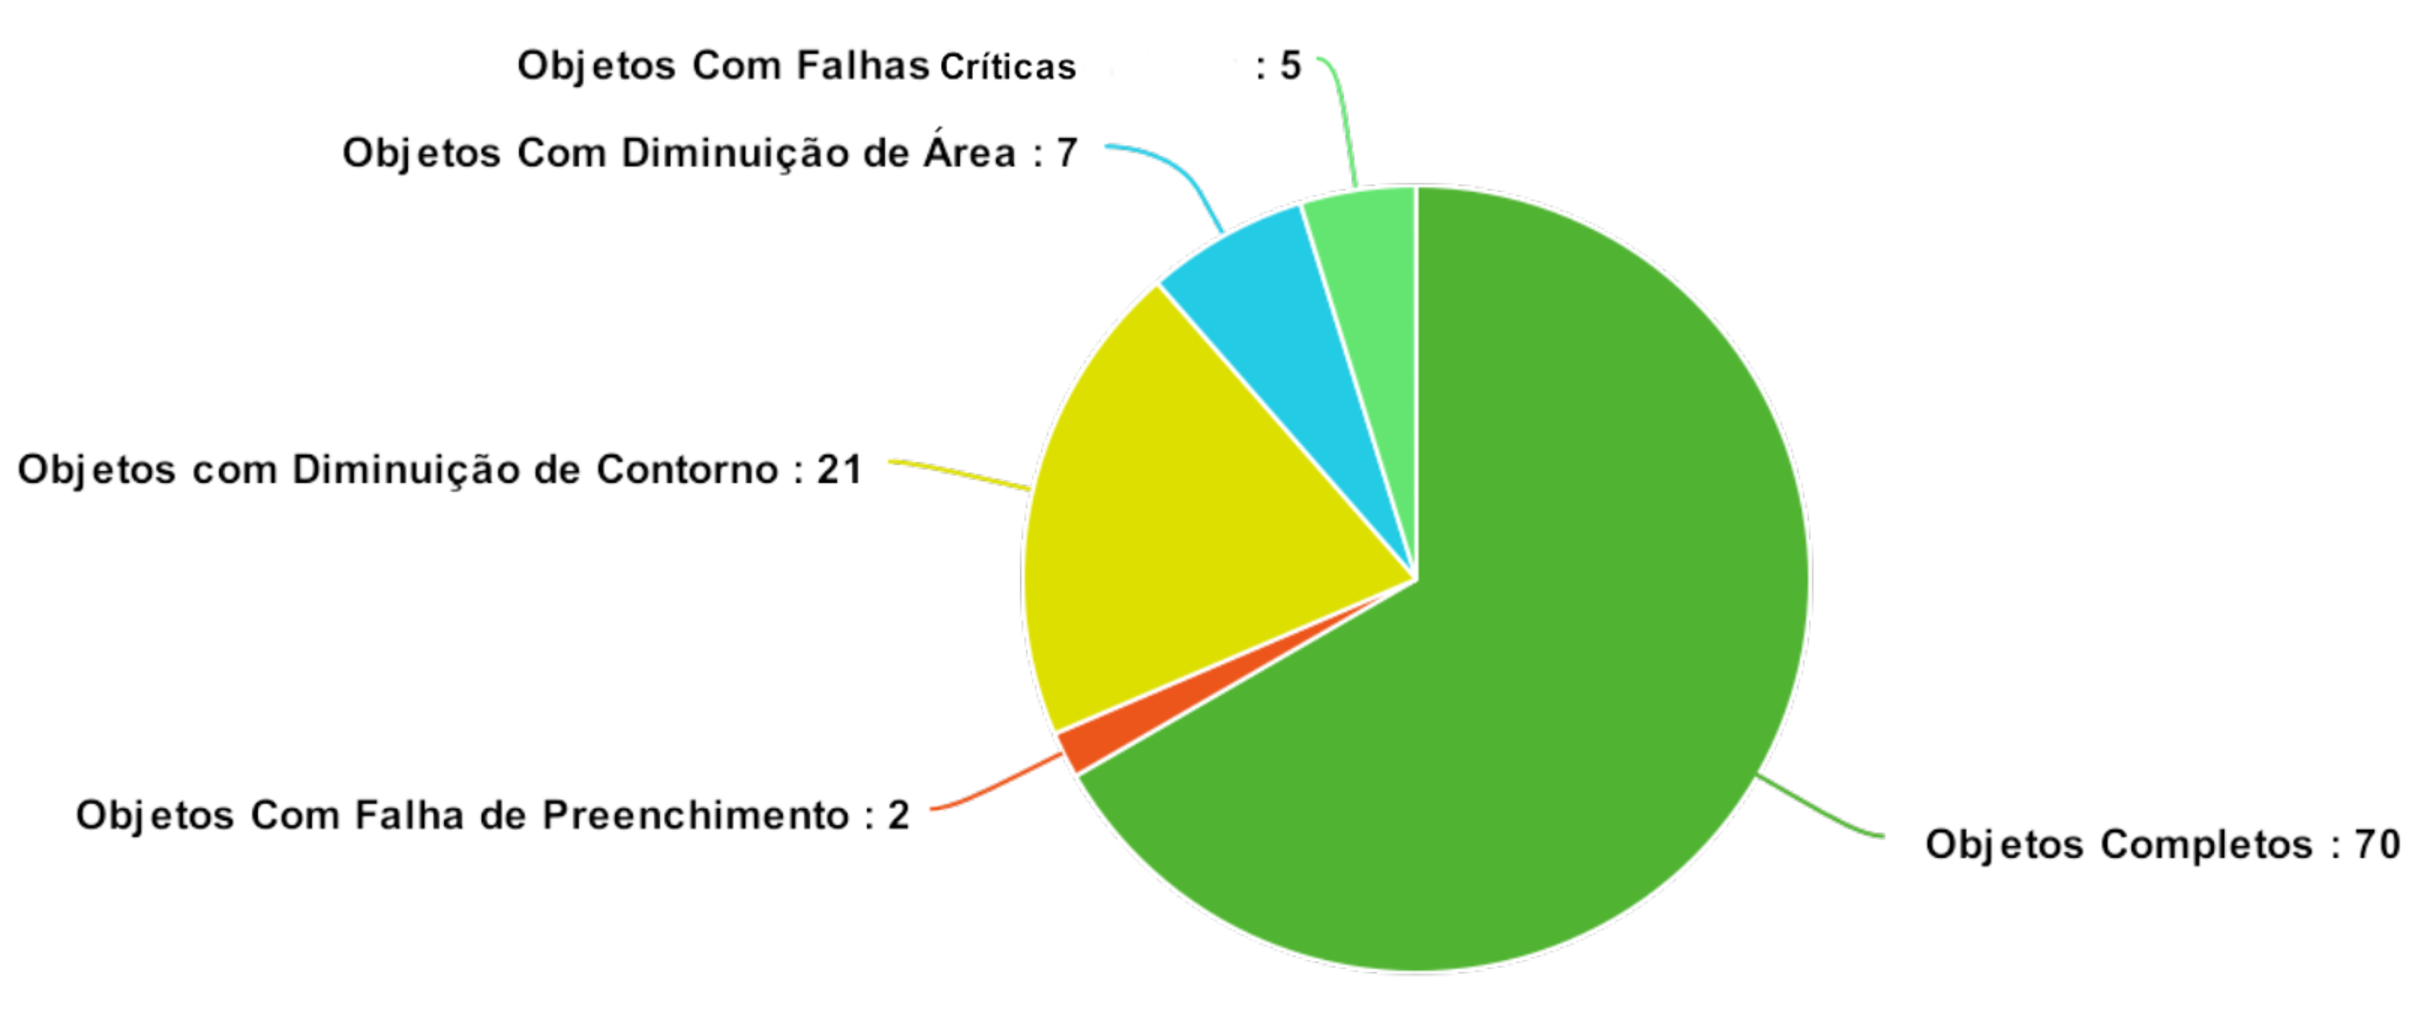
\includegraphics[width=0.8\textwidth]{/testes/graficotestes.pdf}
		\caption{Gráfico de análise do resultado dos testes}
		\label{disposicaoparte}
	\end{figure}
	
	
	Sabendo destes valores, os que podem ser considerados críticos na detecção de objetos por meio da sua cor são \textit{Objetos Com Falhas Críticas} e \textit{Objetos Com Falha de Preenchimento} que juntos somam 6,67\% dos objetos. % Resultados
%%====================================================================================================
% ?????
%====================================================================================================
% TCC
%----------------------------------------------------------------------------------------------------
% Autor				: Jasane Schio
% Orientador		: Gedson Faria
% Co-Orientador		: Angelo Darcy
% Instituição 		: UFMS - Universidade Federal do Mato Grosso do Sul
% Departamento		: CPCX - Sistema de Informação
%----------------------------------------------------------------------------------------------------
% Data de criação	: 01 de Outubro de 2015
%====================================================================================================

\chapter{Conclusão} \label{Cap:Conclusao}

\section{Principais Considerações}
	Foi realizado um estudo dos modelos de cores dentro da biblioteca OpenCV e foram identificados intervalos definidos de cada uma das cores. Seus espectros foram encontrados uma vez que se identificou que, ao contrario do que acontece no mundo real, um pixel na biblioteca assume o  padrão GBR e uma vez convertido ao HSV possui os valores alterados. Assim por meio de experimentação e da ajuda de foruns  disponíveis na internet, se chegou ao melhor espectro para cada cor, categorizando o pixel dentre seus respectivos intervalos. Para serem identificadas as tiras a serem calibrados no campo, utilizou-se a técnica Algoritmo de Canny, que faz a detecção das bordas presentes na imagem. Após serem detectadas as bordas fez-se então uma analise para identificar quais bordas pertencem à mesma tira, é somente após essa analise que as tiras são identificas pela junção de suas respectivas bordas. Assim que identificadas, cada um dos tiras foi analisado de acordo com o estudo das cores para assimilar a qual cor a mesma pertencia, e seus valores comparados para identificar se esta seria um limite do intervalo da cor a qual pertence.

A avaliação dos resultados foi separado em \textbf{Calibração} e \textbf{Teste}. Para ambos foram usadas 7 cores: Amarelo, Azul, Laranja, Rosa, Roxo, Verde e Vermelho. A Calibração durou ao todo aproximadamente 5 minutos e gerou o arquivo \textit{cores.arff} contendo os valores HSV mínimo e máximo para cada cor. Para o Teste foi desenvolvida uma aplicação que faz a exibição das cores de acordo com seus valores no arquivo \textit{cores.arff}. A aplicação mostra uma imagem somente com os objetos da cor selecionada, esta imagem é a que foi usada nos testes do Capitulo 4. Cada objeto de cada cor foi categorizado em: Completo; Com Falha de Preenchimento; Com Diminuição de Contorno; Com Diminuição de Área ou Com Falha Criticas. Das categorias de objetos citadas, as que possuem a área do objeto deformada, o que dificulta sua identificação, são \textit{Falha de Preenchimento} e \textit{Falha Criticas}. Somente tr\^{e}s cores apresentaram estas falhas: Amarelo, com 6,66\%; Vermelho, com 13,33\%; e Rosa, com 26,66\%. De outro modo, somente uma cor não apresentou objetos completos, a cor Rosa. As cores Amarelo, Azul, Verde e Laranja obtiveram mais de 90\% de seus objetos encontrados completamente. A cor Vermelha obteve 53,33\% de seus objetos encontrados e o Roxo 26,66\%. 
Portanto o sistema cobre seu objetivo principal de automatizar o processo de calibração de cores, além da diminuição do tempo de calibração, uma vez que o sistema faz a calibração de todas as cores ao mesmo tempo, o que era feito cor por cor da forma manual.	

\section{Trabalhos Futuros}
Melhorias são indicadas para o sistema tanto na área de detecção de objetos quanto para a categorização de cores. Na detecção de objetos recomenda-se aprimorar a técnica para que não necessitem da subtração de fundo, pois a técnica utilizada neste trabalho infelizmente requer um certo tempo de processamento bem como ação manual, assim sera possível que o sistema se torne 100\% automatizado e ainda mais rápido.

 Quanto a categorização de cores: a aplicação da técnica também para a cor ciano, bem como melhorar os valos de S e V, uma vez que esses estão sendo usados de maneira estática, seria indicado uma melhoria para que os mesmos sejam os valores detectados das tiras de cor, o que necessita de um certo tratamento.
 
Outra indicação de incrementação do projeto seria a conversão do sistema para uma biblioteca modular, para que o mesmo possa ser incorporado em diferentes sistemas de estrategia.  % Conclusão

\cleardoublepage
\phantomsection
\addcontentsline{toc}{chapter}{Referências Bibliográficas}
\bibliographystyle{abnt}
%\bibliographystyle{abnt-num} % Numérico
%\bibliographystyle{abnt-alf} % Autor-Data
%\bibliographystyle{abbrv}
%\bibliographystyle{apalike} 
%\bibliographystyle{ieeetr} % Ordena por ordem de aparição.  
%\bibliographystyle{abbr} % Ordena por ordem alfabetica com nomes abreviados.
%\bibliographystyle{plain} % Ordena por ordem alfabetica com nomes por extenso.
\bibliography{bibliografia.bib} % commented if *.bbl file included.


\addcontentsline{toc}{chapter}{Ap\^endices}
\appendix
%%====================================================================================================
% ?????
%====================================================================================================
% TCC
%----------------------------------------------------------------------------------------------------
% Autor				: Jasane Schio
% Orientador		: Gedson Faria
% Co-Orientador		: Angelo Darcy
% Instituição 		: UFMS - Universidade Federal do Mato Grosso do Sul
% Departamento		: CPCX - Sistema de Informação
%----------------------------------------------------------------------------------------------------
% Data de criação	: 01 de Outubro de 2015
%====================================================================================================

\chapter{Anexos} \label{App:ApendiceA}

a:



\end{document}
